%  ========================================================================
%  Copyright (c) 1985 The University of Washington
%
%  Licensed under the Apache License, Version 2.0 (the "License");
%  you may not use this file except in compliance with the License.
%  You may obtain a copy of the License at
%
%      http://www.apache.org/licenses/LICENSE-2.0
%
%  Unless required by applicable law or agreed to in writing, software
%  distributed under the License is distributed on an "AS IS" BASIS,
%  WITHOUT WARRANTIES OR CONDITIONS OF ANY KIND, either express or implied.
%  See the License for the specific language governing permissions and
%  limitations under the License.
%  ========================================================================
%

% Documentation for University of Washington thesis LaTeX document class
% by Jim Fox
% fox@washington.edu
%
%    Revised 2020/02/24, added \caption()[]{} option.  No ToC.
%
%    Revised for version 2015/03/03 of uwthesis.cls
%    Revised, 2016/11/22, for cleanup of sample copyright and title pages
%
%    This document is contained in a single file ONLY because
%    I wanted to be able to distribute it easily.  A real thesis ought
%    to be contained on many files (e.g., one for each chapter, at least).
%
%    To help you identify the files and sections in this large file
%    I use the string '==========' to identify new files.
%
%    To help you ignore the unusual things I do with this sample document
%    I try to use the notation
%       
%    % --- sample stuff only -----
%    special stuff for my document, but you don't need it in your thesis
%    % --- end-of-sample-stuff ---


%    Printed in twoside style now that that's allowed
%
 
\documentclass [11pt, proquest] {uwthesis}[2020/02/24]
 
%
% The following line would print the thesis in a postscript font 

\usepackage{natbib}
\def\bibpreamble{\protect\addcontentsline{toc}{chapter}{Bibliography}}

\setcounter{tocdepth}{1}  % Print the chapter and sections to the toc

\usepackage{amsmath}
\usepackage{amsthm}
\usepackage{amssymb}
\usepackage{xspace}
\usepackage{natbib}
\usepackage{csvsimple}
\usepackage{microtype}
\usepackage{tikz}
\usepackage{tikz-qtree}
\usepackage{tabularx}
\usepackage{makecell}
\usepackage[ruled,vlined]{algorithm2e}
\usepackage{hhline}
\usepackage{subfigure}
\usepackage{listings}

\usetikzlibrary{hobby,arrows,backgrounds,calc,trees,automata}

\pgfdeclarelayer{background}
\pgfsetlayers{background,main}

\newcommand{\convexpath}[2]{
[   
    create hullnodes/.code={
        \global\edef\namelist{#1}
        \foreach [count=\counter] \nodename in \namelist {
            \global\edef\numberofnodes{\counter}
            \node at (\nodename) [draw=none,name=hullnode\counter] {};
        }
        \node at (hullnode\numberofnodes) [name=hullnode0,draw=none] {};
        \pgfmathtruncatemacro\lastnumber{\numberofnodes+1}
        \node at (hullnode1) [name=hullnode\lastnumber,draw=none] {};
    },
    create hullnodes
]
($(hullnode1)!#2!-90:(hullnode0)$)
\foreach [
    evaluate=\currentnode as \previousnode using \currentnode-1,
    evaluate=\currentnode as \nextnode using \currentnode+1
    ] \currentnode in {1,...,\numberofnodes} {
  let
    \p1 = ($(hullnode\currentnode)!#2!-90:(hullnode\previousnode)$),
    \p2 = ($(hullnode\currentnode)!#2!90:(hullnode\nextnode)$),
    \p3 = ($(\p1) - (hullnode\currentnode)$),
    \n1 = {atan2(\y3,\x3)},
    \p4 = ($(\p2) - (hullnode\currentnode)$),
    \n2 = {atan2(\y4,\x4)},
    \n{delta} = {-Mod(\n1-\n2,360)}
  in 
    {-- (\p1) arc[start angle=\n1, delta angle=\n{delta}, radius=#2] -- (\p2)}
}
-- cycle
}
\tikzset{
  leaf/.style={sibling distance=5mm}
}

% ==========   Local defs and mods
\definecolor{uwpurple}{RGB}{128,0,128}
\definecolor{darkgreen}{RGB}{0,64,0}
%\newcommand{\jln}[1]{\textcolor{uwpurple}{\textit{[{#1} --JLN]}}}
\newcommand{\jln}[1]{\textcolor{uwpurple}{}}
\newcommand{\sak}[1]{\textcolor{olive}{\textit{[{#1} --SK]}}}
\newcommand{\aba}[1]{\textcolor{darkgreen}{\textit{[{#1} --AA]}}}
\newcommand{\rb}[1]{\textcolor{blue}{\textit{[{#1} --RB]}}}

\newcommand{\modified}[1]{\textcolor{black}{{#1}}}
\newcommand{\modifiedagain}[1]{\textcolor{black}{{#1}}}

\newcommand{\trsone}[0]{TRS1}
\newcommand{\trstwo}[0]{TRS}
\newcommand{\goallang}[0]{\mathcal{L}}
\newcommand{\termlang}[0]{T(\Sigma,V)}
\newcommand{\goalorder}[0]{>_{\phi}}
\newcommand{\st}[0]{\;.\;}

\newcommand{\hmax}[0]{\texttt{max}}
\newcommand{\hmin}[0]{\texttt{min}}
%\newcommand{\rewrites}[0]{\mathop{\rightarrow}\limits_{\scriptscriptstyle{R}}}
\newcommand{\rewrites}[0]{\:\rightarrow_{R}\:}
%\newcommand{\rewrites}[0]{\longrightarrow}
%\newcommand{\rewrites}[0]{\rightharpoonup}
\newcommand{\pred}[0]{\textrm{ if }}
\newcommand{\hfalse}[0]{\texttt{false}}
\newcommand{\htrue}[0]{\texttt{true}}
\newcommand{\hsel}[0]{\texttt{select}}
\usepackage{syntax}

\newtheorem*{remark}{Remark}
\newtheorem{assumption}{Assumption}

%% Macros for quantities
\newcommand{\NumApps}{{\color{black} 10}\xspace}
\newcommand{\NumRulesFixed}{{\color{black} 4}\xspace}
\newcommand{\NumPredicatesRelaxed}{{\color{black} 17}\xspace}
\newcommand{\NumOrderingProblems}{{\color{black} 8}\xspace}
\newcommand{\NumRulesSynthesized}{{\color{black} 4127}\xspace}
\newcommand{\NumOpSequences}{{\color{black} 6246}\xspace}
\newcommand{\NumFailureExamples}{{\color{black} 61000}\xspace}
\newcommand{\NumSimplifiedExpressions}{{\color{black} 195371}\xspace} 
\newcommand{\NumBugsAutomated}{{\color{black} 5}\xspace}
\newcommand{\NumOriginalRules}{{\color{black} 999}\xspace}
\newcommand{\NumZdivCoqProvedRules}{{\color{black} 141}\xspace}
\newcommand{\NumZdivFalseRules}{{\color{black} 44}\xspace}
\newcommand{\NumZdivRelaxedPredicates}{{\color{black} 37}\xspace}

\newtheorem{theorem}{Theorem}[section]

% --- sample stuff only -----
% These format the sample code in this document

\usepackage{alltt}  % 
\newenvironment{demo}
  {\begin{alltt}\leftskip3em
     \def\\{\ttfamily\char`\\}%
     \def\{{\ttfamily\char`\{}%
     \def\}{\ttfamily\char`\}}}
  {\end{alltt}}
 
% metafont font.  If logo not available, use the second form
%
% \font\mffont=logosl10 scaled\magstep1
\let\mffont=\sf
% --- end-of-sample-stuff ---
 
\usepackage{hyperref}


\begin{document}
 
% ==========   Preliminary pages
%
% ( revised 2012 for electronic submission )
%

\prelimpages
 
%
% ----- copyright and title pages
%
\Title{Augmenting and Synthesizing Term Rewriting Systems}
\Author{Julie L. Newcomb}
\Year{2021}
\Program{Computer Science and Engineering}

\Chair{Name of Chairperson}{Title of Chair}{Department of Chair}
\Signature{First committee member}
\Signature{Next committee member}
\Signature{etc}

\copyrightpage

\titlepage  

 
%
% ----- signature and quoteslip are gone
%

%
% ----- abstract
%


\setcounter{page}{-1}
\abstract{%
  Halide is a domain-specific language for high-performance image processing and tensor computations, widely adopted in industry.
  Internally, the Halide compiler relies on a term rewriting system to
  prove properties of code required for efficient and correct compilation.  This rewrite
  system is a collection of handwritten transformation rules 
  that incrementally rewrite expressions into simpler forms; the system requires high performance 
  in both time and memory usage to keep compile times low,
  while operating over the undecidable theory of integers.
  In this work, we apply formal techniques to prove the correctness of existing
  rewrite rules and provide a guarantee of termination. Then,
  we build an automatic program synthesis system 
  in order to craft new, provably correct rules from failure cases
  where the compiler was unable to prove properties. We identify and fix
  \NumRulesFixed incorrect rules as well as \NumOrderingProblems rules which
  could give rise to infinite rewriting loops.
  %% We run our synthesis process against 
  %% a large suite of failed proofs from compiler output, synthesizing a new body
  %% of rules that improves the system's proving power as evaluated on realistic
  %% benchmarks.
  %% The automated system can replace tedious human effort required to craft new rules
  %% in response to user-reported bugs.  We demonstrate that the new
  %% term rewriting system is provably sound, more robust, and more general, without
  %% slowing down the compiler.
  We demonstrate that the synthesizer can produce better rules than hand-authored ones in five bug fixes, and describe four cases in which it has served as an assistant to a human compiler engineer. We further show that it can proactively improve weaknesses in the compiler by synthesizing a large number of rules without human supervision and showing that the enhanced ruleset lowers peak memory usage of compiled code without appreciably increasing compilation times.

  We then turn from the goal of improving a handwritten term rewriting system to synthesizing an entirely new one. We argue that an artifact from a TRS termination proof, a special type of order over terms known as a reduction order, is an effective and expressive means of writing a specification for a term rewriting system. We demonstrate its own on a case study of another component of the Halide compiler called the variable solver. We present a synthesis process that takes a specification written in the form of a reduction order and a set of sample input expressions and produces a new ruleset. Furthermore, we show that we can use this synthesis process to allow users to experiment with different specifications by automatically generating new TRSs and evaluating them empirically, without ever handing to write a rule by hand.
}
 
%
% ----- contents & etc.
%
\tableofcontents
%\listoffigures
%\listoftables  % I have no tables
 
%


%
% ----- acknowledgments
%
%\acknowledgments{% \vskip2pc
  % {\narrower\noindent
%  -
  % \par}
%}

%
% ----- dedication
%
%\dedication{\begin{center}-\end{center}}

%
% end of the preliminary pages
 
 
 
%
% ==========      Text pages
%

\textpages

% ========== chapters
\chapter{Introduction}
\label{sec:intro}

Term rewriting systems are a useful tool in the construction of compilers. They are a succinct and efficient way of executing program reasoning tasks, and can give extremely fast performance. 

However, term rewriting systems can be challenging both to develop and to maintain. As the path of execution for inputs can vary greatly, it can be difficult for developers to reason about how the various rules in the system interact as a whole. Adding, altering, or deleting a rule can have unforeseen consequences. Even if a TRS contains unsound rules, it may give correct results on all but a few inputs, and when the error is detected it can be difficult to track down which rules is responsible. A slight change to the ruleset can make it possible for rules form cycles, causing the system to fail to terminate on some inputs. 

The task of authoring these systems is even more challenging when the language of input expressions is in an undecidable theory. Since a term rewriting system in such a language cannot be complete, it is hard to know if a given system is optimal or if some change would improve its performance, degrade it, or perhaps make no difference at all.

In this work, we propose to show how authoring and maintaining term rewriting systems can be made easier through the use of formal methods and program synthesis. We will demonstrate how these techniques can support all degrees of human involvement: from verifying and strengthening existing term rewriting systems, to bootstrapping term rewriting systems from a specification and a set of seed axioms, to synthesizing a new ruleset entirely from scratch.

In this work we make the following contributions:

\begin{itemize}
    \item \emph{We show formal methods and program synthesis can usefully assist the authors of term rewriting systems.} Formal proofs of soundness and guarantees of termination can find bugs in large, widely-deployed term rewriting systems, and automatic program synthesis can be used to find new rewrite rules to augment these systems.
    \item \emph{We present an effective means of encoding a specification for the synthesis of term rewriting systems.} Besides providing a proof of termination, we claim that reduction orders can serve as a useful formalization of the intent behind a term rewriting system, and can be used as a specification when synthesizing rewrite rules.
\end{itemize}

We evaluate our work in two case studies. In the first, we investigate the first claim by using formal methods to enhance a pivotal term rewriting system within the Halide compiler called the simplifier. We found that we were able to identify bugs, prove the absence of future errors, and increase the rewriting power of the system. We review our evaluation of the first claim in section~\ref{sec:prior}. 

In the second case study, we take a look at a smaller and less mature term rewriting system in Halide called the variable solver. Previously, we synthesized new rules for the simplifier largely guided by its large existing ruleset. Here, we plan to evaluate our proposed means of writing specifications for term rewriting system by synthesizing a ruleset entirely from scratch. We lay out our means of writing specification and our evaluation of the synthesized rulesets in section~\ref{intro:varsolver}.

\section{Maintaining an existing term rewriting system}
\label{sec:prior}

The Halide compiler contains a hand-authored term rewriting system commonly called the simplifier. It is used in many cases within the compiler for making expressions shorter and in a form better suited to downstream uses. Sometimes the simplifier is used as a prover: the truth value of an expression is checked by rewriting it with the simplifier to see if it will be rewritten to the constant true. At the time we began this work, the simplifier was fairly mature: it had been deployed in production for over a year, was both unit tested and fuzz tested, and comprised almost a thousand rules.

Is it necessary to apply formal methods to the authoring of term rewriting systems? In previous work, we showed that applying formal methods can identify and remedy real issues in the simplifier TRS. Conversely, we observe that implementing expression-transforming code as a term rewriting system is useful precisely because it allows easy integration with formal methods. We also show that we can improve this term rewriting system by synthesizing new rewrite rules automatically and that this synthesis process can be used in the compiler's development process. We first provide a proof of soundness and of termination, and then detail the rule synthesis process below. This work has been published at OOPSLA 2020~\cite{newcomb2020verifying}.

\subsection{Proof of soundness}
First, we formally verify that each rule in the Halide simplifier ruleset is semantics-preserving, demonstrating that proofs of soundness are possible despite the lack of a 
decision procedure for our theory. We do this by modeling the semantics of the Halide expression language in SMT2. We then implemented a pretty-printer to translate each rule in the simplifier ruleset to an SMT query to be checked by the solver Z3~\cite{de2008z3}. About 12\% of the ruleset could not be verified by Z3, and we proved those rules correct by hand using the proof assistant Coq~\cite{Coq19}. Even though the code had been deployed for over a year and had been fuzz-tested, we found that four of the existing rules were incorrect and submitted patches. In constructing the Coq proofs, we also noticed that 17 rules had predicates that were overly conservative, and submitted patches for the relaxed predicates as well.

While this project was ongoing, the Halide semantics for division was changed: division by zero was no longer undefined behavior, but now returned zero. It was simple for us to amend our modeled semantics and rerun rule verification in Z3. Again about 12\% of the ruleset had to be hand-proven using Coq, but we were able to leverage many of the existing proofs from our previous verification. Our verification identified 44 rules which were not correct under the new semantics and 37 rules whose predicates could be relaxed under the semantics change. This shows the value of our formal methods infrastructure, which allowed Halide developers to push a fairly major change with a higher degree of confidence in the soundness of the simplifier than could have been achieved with either manual testing or fuzzing.

\subsection{Proof of termination}
The Halide simplifier algorithm successively applies rewrite rules until the resulting expression can no longer be rewritten. Thus, if some sequence of rewrites to some input expression can form a cycle, the simplifier algorithm will not terminate. These non-termination errors have been observed in the past (resulting in the compiler throwing a stack overflow error and crashing). Without a specific input expression on which to reproduce a cycle, it is very difficult to examine a set of around a thousand rules and find a subset on which a cycle could occur; even once a cycle has been identified, it is difficult to know the best way to repair it. The ruleset was thus very brittle; deleting, altering, or reordering existing rules has caused new non-termination errors in the past as well.

A term rewriting system can be proven to terminate using a formalism called a \emph{reduction order}~\cite{baader1999term}. A reduction order is an order over a language of terms; if for every rule in a term rewriting system, we can show that the rule's left-hand side is strictly greater than the right-hand side in this order, then we know that there can be no set of rules that can form a cycle, and thus the ruleset must always terminate. A reduction order is distinguished by a few special properties to ensure that these ordering holds no matter how input expressions are matched to the left-hand side term, as well as when a rule is used to rewrite a subterm inside of a larger input expression; see ~\cite{newcomb2020verifying} for full details.

We devised a reduction order that fit as many of the existing simplifier rules as possible. Eight rules could not be fit to our ordering, and we submitted patches to either delete or modify them. Once this was done, not only was a class of bugs eliminated, but the ruleset could now be safely modified without fear of introducing new non-termination behavior. It was also now safe to add any new rule so long as the rule conformed to the reduction order. 

We observe that this reduction order serves to encode the meaning of simplification in the context of the Halide TRS
by formalizing what it means for a rule to usefully modify an expression.  While
many notions of ``simpler'' are possible, we encode the specific criteria for Halide
expressions by defining an \emph{ordering} over the left-hand and right-hand terms of 
the rules in the TRS that captures the intentions behind the rewrites. This ordering 
means that every local change caused by the application of a rewrite rule moves the 
expression in some useful direction. By composing several orders lexicographically, 
we can express many different intuitions about what makes an expression simpler in a
defined priority: we may want to remove as many vector operations as possible, 
then reduce the overall size of the expression, and so on. Maintaining this order as 
an invariant over any future rules means any additions to the ruleset will not undo 
progress made by existing rules.

\subsection{Strengthening the ruleset}
We can empirically observe that the simplifier ruleset is not sufficiently powerful to deal with all expressions it may be called upon, by instrumenting the compiler and logging any expressions that the simplifier cannot further solve. In the past, ruleset authors might look at these failed expressions and write rules to address them by hand. In ~\cite{newcomb2020verifying}, we automated this progress by synthesizing these rules instead.

However, even
given the constraints imposed by the termination order, the space of equivalences 
in the Halide expression language is infinitely large. How do we choose which  
rules to add? We observe that there is some bias on the distribution of expressions 
seen by the compiler on realistic inputs over the full expression space. We take advantage 
of this bias by gathering expressions from realistic compilations on which the current 
TRS is ``stuck'' and can make no further progress. We synthesize rules through a pipeline that takes these expression as input and uses CEGIS loops to synthesize an equivalent right-hand side and (if necessary) a predicate guard that indicates when it is safe to apply 
the rule. Our pipeline produces more general rules by mining input expressions for larger patterns and by replacing constants with fresh variables. We also find variants on synthesized rules by applying associativity and commutitativity laws to their left-hand sides. We choose candidate left-hand sides 
for rules from this corpus and synthesize equivalent right-hand terms that obey the 
termination order. In our experiments, we found that our synthesis pipeline could produce patches to ruleset bugs as good or better than those that were authored by hand. We also observed Halide developers integrating the rule synthesizer into their workflow. Our synthesis procedure is also capable of finding large numbers of useful rules without
human oversight; although the existing compiler is mature 
and well-tuned for our suite of benchmarks, we show some performance 
gains without increases in compilation time when our newly synthesized suite 
of rules is added to the TRS. 

 

\section{Synthesizing a new term rewriting system}
\label{intro:varsolver}

For the Halide simplifier, we synthesized individual rules to augment an already mature term rewriting system. Next, we demonstrate the synthesis of term rewriting systems completely from scratch. We do this using the Halide \emph{variable solver} as a case study. The variable solver takes a Halide expression and a variable found within that expression (the \emph{target variable}) and attempts to eliminate as many instances of that variable as it can and isolate the variable to one side of the expression as best it can. (If the expression is an equality, this would consitute `solving' the expression for the chosen variable.) 

An idealized version of our proposed synthesis procedure is laid out in algorithm~\ref{algo:synthesis}. This procedure requires a goal function, which returns true if a term is in some desired form and false otherwise; a semantic equivalence relation; and a reduction order over terms, as well of a set of training expressions $E$, which should be representative of the types of expressions the term rewriting system will take as input and a set of test expressions $S$ on which to evaluate the behavior of the term rewriting system.

The key input to the synthesis procedure is the reduction order over terms, which serves as a specification for the synthesis of rules. The reduction order is a means of formalizing either the intent of the term rewriting system\textemdash the form into which the TRS should rewrite expressions\textemdash or the strategy by which the TRS will rewrite expressions to be closer to the desired form. While TRS authors are likely to have good intuition as to what rewriting strategy their system should employ, choosing the best reduction order for the task is still not a trivial exercise. Our synthesis process gives users the chance to experiment and determine which reduction order serves their purpose best; rather than hand-turning rules, they can synthesize a ruleset entirely from scratch for a given reduction order and evaluate it directly.

We use the Halide variable solver as a case study to demonstrate how synthesis can be used to evaluate reduction order specifications. We lay out the refined synthesis algorithm, with some discussion of how best to search the space of candidate rules, and show how reduction orders can be encoded efficiently as metasketches. We evaluate our claims by synthesizing two rulesets from two different reduction orders in a fully automated way and evaluate their performance against the existing handwritten solver on a suite of benchmarks.


\chapter{Background}
\label{chapter:overview}

We define term rewriting systems and give some background. We then discuss the use of term rewriting systems in the Halide compiler and describe the two main such systems, the \emph{simplifier} and the \emph{variable solver}. We describe the rewriting algorithm used by the Halide compiler and discuss the requirements that led to its design choices. 

The Halide compiler contains term rewriting systems operating over the space of Halide expressions (see appendix~\ref{a:grammar} for
the full Halide expression grammar). The language of Halide expressions
operates over vectors and scalars of integers, booleans, and real values.  However, in
this work we concentrate on the TRS as it applies to integer and boolean values, for
both vectors and scalars, because the most important uses of the TRS within the compiler
apply to these types.  In this section, we give some background on term rewriting systems.
We then describe how the Halide compiler uses term rewriting systems as reasoning engines
and the design decisions that motivate the custom rewriting engine, as well as the scope
of our work.

\section{Term Rewriting Systems}

Term rewriting systems~\citep{gorn1967} are sets of \textit{rewrite rules} used to transform expressions into a new form.  Such systems are widely
used in theorem proving~\citep{baader1999term} and abstract interpretation~\citep{cousot1977abstract, cousot1979systematic}.

Terms are defined inductively over a set of variables $V$ and a set of function symbols $\Sigma$. Every variable $v \in V$ is a term, and for any function symbol $f \in \Sigma$ with arity $n$ and any terms $t_1, ..., t_n$, the application of the symbol to the terms $f(t_1, ..., t_n)$ is also a term. (Constants are considered zero-arity functions.) We refer to the set of terms constructed from the variables $V$ and the function symbols $\Sigma$ as $T(\Sigma, V)$.

A \emph{rewrite rule} is a directed binary relation $l \rewrites r$ such that $l$ is not a variable, and all variables present in $r$ are also present in $l$ (i.e., $\mathcal{V}ar(l) \supseteq \mathcal{V}ar(r)$). A set of rewrite rules is called a \emph{term rewriting system}.

Consider a set of terms $T(\Sigma, V)$ such that $\Sigma = \{\clubsuit, \diamondsuit\}$ and $V$ is an infinite set of variables. Let the term rewriting system $R$ consist of a single rule:

\[ R = \{ x_1 \clubsuit x_2 \rewrites x_1 \diamondsuit x_2 \} \]
We use $R$ to rewrite the term

\[ 
(y_1 \diamondsuit y_1) \clubsuit (y_2 \clubsuit y_3)
\]
The first step is matching; we find a substitution that will unify the left-hand side (LHS) of the rule with the term we are rewriting. Here, one possible substitution is:

\[
\{ x_1 \mapsto (y_1 \diamondsuit y_1), x_2 \mapsto (y_2 \clubsuit y_3) \}
\]
We then apply this substitution to the right-hand side (RHS) of the rule to obtain the rewritten version of the original term:

\[ 
(y_1 \diamondsuit y_1) \diamondsuit (y_2 \clubsuit y_3)
\]


\section{Term rewriting systems in the Halide compiler}



\begin{figure*}
\begin{tabular}{cccc}

%\Tree [.+ [.- [.min a b ] [.max c c ] ] [.max c c ]]
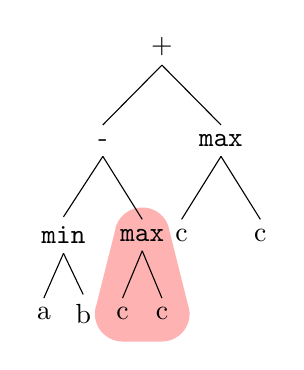
\begin{tikzpicture}[level distance=12mm]
\tikzstyle{level 1}=[sibling distance=15mm]
\tikzstyle{level 2}=[sibling distance=10mm]
\tikzstyle{level 3}=[level distance=10mm,sibling distance=5mm]


%\Tree [.+ [.- [.min a b ] c ] [.max c c ]]
\node (+) {+}
  child { node (-) {-}
    child { node (min) {\hmin}
      child {node (a) {a}}
      child {node (b) {b}}
    }
    child { node (max2) {\hmax}
      child {node (c4) {c}}
      child {node (c5) {c}}
    }
  }
  child { node (max) {\hmax}
    child { node (c2) {c}}
    child { node (c3) {c}}
  };
\begin{pgfonlayer}{background}
\fill[red,opacity=0.3] \convexpath{c4,max2,c5}{10pt};
\end{pgfonlayer}
\end{tikzpicture}

&
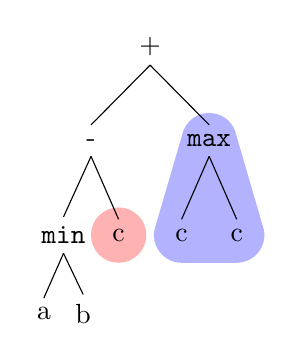
\begin{tikzpicture}[level distance=12mm]
\tikzstyle{level 1}=[sibling distance=15mm]
\tikzstyle{level 2}=[sibling distance=7mm]
\tikzstyle{level 3}=[level distance=10mm,sibling distance=5mm]
%\Tree [.+ [.- [.min a b ] c ] [.max c c ]]
\node (+) {+}
  child {  node (-) {-}
    child { node (min) {\hmin}
      child {node (a) {a}}
      child {node (b) {b}}
    }
    child { node (c) {c}}
  }
  child { node (max) {\hmax}
    child { node (c2) {c}}
    child { node (c3) {c}}
  };
\begin{pgfonlayer}{background}

\fill[blue,opacity=0.3] \convexpath{c2,max,c3}{10pt};
%\fill[red,opacity=0.3] \convexpath{c}{10pt};
\draw[fill=red,opacity=0.3,draw=none](c) circle (10pt);

\end{pgfonlayer}
\end{tikzpicture}
&
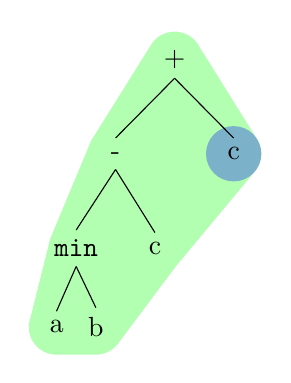
\begin{tikzpicture}[level distance=12mm]
\tikzstyle{level 1}=[sibling distance=15mm]
\tikzstyle{level 2}=[sibling distance=10mm]
\tikzstyle{level 3}=[level distance=10mm,sibling distance=5mm]
%\Tree [.+ [.- [.min a b ] c ] c ]
\node (+) {+}
  child { node (-) {-}
    child { node (min) {\hmin}
      child {node (a) {a}}
      child {node (b) {b}}
    }
    child { node (c) {c} }
  }
  child { node (c2) {c}};



  \begin{pgfonlayer}{background}
\fill[green,opacity=0.3] \convexpath{b,a,min,-,+,c2,c}{10pt};
\draw[fill=blue,opacity=0.3,draw=none](c2) circle (10pt);
%\draw[red,fill=blue,opacity=0.3](c2.north) to[closed,curve through={($(c2.north east)!1.0!(c2.south east)$) .. ($(c2.south west)!1.0!(c2.north west)$)}] (c2.north);
\end{pgfonlayer}
\end{tikzpicture}
&
\vspace{0pt}
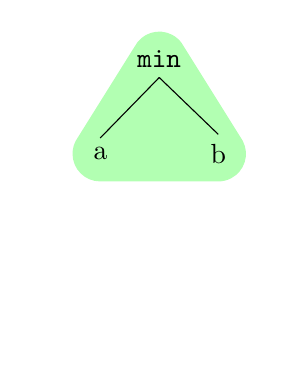
\begin{tikzpicture}[level distance=12mm]
\tikzstyle{level 1}=[sibling distance=15mm]
\tikzstyle{level 2}=[sibling distance=10mm]
\tikzstyle{level 3}=[level distance=10mm,sibling distance=5mm]
\node (min) {\hmin}
  child { node (a) {a}
     % [red,opacity=0.0]
    child {     [red,opacity=0.0] node (fake1) {f}
      child {    [red,opacity=0.0] node (fake2) {f}}
      child {    [red,opacity=0.0] node (fake3) {f}}
    }
    child {     [red,opacity=0.0] node (fake4) {f}
    [red,opacity=0.0]
    child { [red,opacity=0.0] node (fake) {f}}
    child { [red,opacity=0.0] node (fake2) {f}}
    }
  }
  child { node (b) {b}
     % [red,opacity=0.0]
    child {     [red,opacity=0.0] node (fake5) {f}}
    child {     [red,opacity=0.0] node (fake6) {f}}
  };
  \begin{pgfonlayer}{background}
\fill[green,opacity=0.3] \convexpath{a,min,b}{10pt};
\end{pgfonlayer}

\end{tikzpicture} \\
(i) & (ii) & (iii) & (iv)
\end{tabular}
\caption{We demonstrate the Halide rewriting algorithm using a TRS $R = \{\hmax(x, x) \rewrites x, (x - y) + y \rewrites x\}$ and an expression $\hmin(a,b) - \hmax(c,c) + \hmax(c,c)$. The algorithm attempts to simplify all subtrees bottom up; here, no rule applies to $\hmin(a,b)$ so it is not changed. Next (i), rule 1 rewrites $\hmax(c,c)$ to $c$. No rule applies to $\hmin(a,b) - c$, so we move to the rightmost subtree and rewrite again (ii) to obtain $c$ from $\hmax(c,c)$. Finally, we consider the entire tree $\hmin(a,b) - c) + c$ (iii) and apply rule 2 to produce $\hmin(a,b)$. No rules match this expression, so we are left with $\hmin(a,b)$ (iv).}
\label{fig:algoexample}
\end{figure*}

\subsection{The Halide rewriting algorithm}
\label{sec:customalgo}

In a term rewriting system, a single rule may be able to match an input expression in 
multiple ways, and there may be multiple rules in the ruleset which could be used 
to rewrite the expression. A term rewriting algorithm might choose one of many alternatives 
and later backtrack if it turns out not to be fruitful; it might make use of 
heuristics to choose a next step; it might exercise all the alternatives and keep 
the results in equivalence classes, as in an e-graph. The Halide term rewriting algorithm
keeps only one expression in state and applies rules greedily, in a fixed priority.
This is very fast and requires very little memory; the tradeoff is that the algorithm 
may pick the ``wrong'' rule and have no way of undoing that decision. 
Since the rewriter is invoked thousands of times with each call of the compiler, 
it chooses to sacrifice some solving power in exchange for performance.

The Halide term rewriting algorithm simplifies an input expression in a
depth-first, bottom-up traversal of the expression DAG. At each node, it 
uses the root node to pick a list of rules, then
attempts to match the subtree expression with the rule LHSs in a fixed priority. Matching
is performed purely syntactically, using C++ template metaprogramming.
 Halide rewrite rules contain special metavariables,
called \emph{symbolic constants}, that can match only with constant values; all other
variables can match any subterm as usual.
When a match is found, the algorithm rewrites the
subtree expression using the RHS of that rule, and then attempts to simplify the
subtree expression again. If no rule matches the subtree, the traversal
continues; when the entire expression cannot be simplified further, the
rewritten expression is returned. See Figure~\ref{fig:algoexample} for a worked
example.

The rewrite rules optionally contain a compile-time predicate guard. 
These guards contain only symbolic constants\footnote{Existing 
rules sometimes have predicates that check if
  non-constant variables can be shown to have certain properties at compile
  time, but these are expensive and used sparingly.}; when the LHS of a rule
matches an expression, its guard is evaluated and only if it
is true will the rewrite be applied.

Halide rewrite rules are applied in a fixed priority, organized so that the TRS 
first attempts very basic rules such as constant folding, then tries more specific 
rules before more general ones. (We do not evaluate the current rule priority in this work.)

Associativity and commutativity laws are particularly troublesome for term rewriting systems. 
For one expression $e$, the number of semantically equivalent expressions grows 
exponentially in terms of the number of AC operations $e$ contains. Some term rewriting 
systems perform a full \emph{AC matching} step during rewriting. Halide's TRS does not
perform this matching, but instead
includes multiple AC variations of rules.
However, a small number of Halide's rewrite rules have the effect of canonicalizing some commutative
expressions. (For example, if a commutative expression has a multiplication as its 
first operand and a subtraction as its second operand, a rule will switch their positions.)
These rules are all early in the application priority, so later rules can rely on
expressions having a quasi-canonical form.

\subsubsection{Why Not Z3?}
\begin{table}
\caption{We compare the performance of Z3 and the Halide TRS in proving a set of 4304 expressions gathered from realistic compiler output. Note that expressions in the ``not proven'' column include expressions that are true but not found to be so by the solvers as well as expressions that are not true. }
\centering
\begin{tabular}{l|r|r|r}
Tool & Runtime & Proven expressions & Not proven \\
\hline
Z3 & 7m29s & 1125 & 3179 \\
Halide TRS & 2s & 885 & 3419 
\end{tabular}
\label{tab:simplifiervsz3}
\end{table}


Given that we make use of the Z3 solver~\citep{de2008z3} for both verification and synthesis, it is natural to ask why Halide could not simply call Z3 for simplification. Z3 is the product of extensive development and is a very powerful, general-purpose solver. However, the Halide term rewriting system has a few key properties that Z3 does not: deterministic output, low memory and compute requirements, and domain-specific optimizations.

As discussed above, the Halide compiler must return the same schedule every time the same pipeline is run. Z3 can fix a random seed, but long-running queries may complete on a more powerful server while timing out on a different machine.

While the Halide algorithm is less powerful than Z3, its deterministic, greedy rule application strategy
gives it a smooth performance curve, whether it succeeds or fails in simplifying an input expression.
A solver like Z3 tends to give very good performance most of the time but gets bogged down in difficult cases, requiring the use of timeouts. The Halide algorithm ``fails fast'': on an input expression which does not match any rule,  the Halide algorithm will complete in time linear to the size of the expression, taking on the order of one CPU cycle per term in the expression per rule in the TRS. To demonstrate this performance tradeoff, we gathered 4304 expressions from queries the Halide compiler made when compiling realistic pipelines, including provably true expressions and expressions that are not provably true. Z3 could prove more expressions true (within a 60 second timeout), but was starkly less performant. As shown in Table~\ref{tab:simplifiervsz3}, Z3 took over 7 minutes to check the set of expressions while the Halide TRS took just 2 seconds. This set of expressions is much smaller than the number of calls the compiler makes to the rewriter in compiling a single pipeline.

Because the Halide algorithm at every step chooses one rule to apply to the single expression it is working on, it scales well in terms of the number of rules in the TRS. See Section~\ref{ssec:compilationspeed} for an evaluation of the effects of adding newly synthesized rules on the performance of the compiler. 

Finally, although Z3 can simplify expressions, simply reducing the size of an expression is not necessarily the goal for the compiler. For example, gathering like terms in some cases can actually prevent Halide or LLVM optimizations from applying. The Halide rewriter uses a domain-specific strategy to guide expressions into more optimizable forms and can be changed or tuned as needed if further optimizations are discovered. 

\subsection{Completeness of the Halide TRS}
\label{sec:completion}

We know by observation that the Halide simplifier TRS cannot prove certain equalities 
that are in fact true, or reduce certain expressions that can be further simplified. 
Our goal is to learn new rules that would strengthen the TRS and allow it to make
further progress on these ``stuck'' expressions. This goal seems similar to that of 
\emph{completion}, which constructs a decision procedure through syntatic rewrites
for a set of identities. We do not use completion directly, although
our synthesis algorithm could be considered analogous to completion in some ways.

In the standard Knuth-Bendix completion algorithm~\citep{knuth1983simple}, we take a
finite set of identities $E$ and a reduction order $>$ on terms as inputs; if successful, the
algorithm will return a finite, convergent set of rules $R$ that is equivalent to 
$E$. The algorithm may also fail, or fail to terminate. At each step the algorithm
maintains a set of identities and a set of rules, both of which can be updated; the 
algorithm may transform an identity into a new rule, find a new identity as a 
consequence of the ruleset, or use the present ruleset to refine either an identity 
or a rule. The algorithm runs until the ruleset has converged; specific implementations
may use some conditions under which to terminate with a failure.

No finite set of identities exists for the theory of integers. We could
fix a set of identities to use in a completion procedure, but choosing these axioms
is a non-trivial task. One issue is that the theory contains axioms such as commutativity;
an identity such as $x + y \equiv y + x$ cannot be oriented by any possible reduction 
order, so our completion algorithm cannot make use of this fact. Another is that any
sufficiently powerful set of identities would almost certainly result in a non-terminating
completion procedure.  In addition, even if we use a subset of the Halide TRS for our
identities (thus yielding a confluent Halide TRS), our experience shows that many
failures in the compiler's use of the TRS are due to missing semantic facts that are not
derivable from the current Halide ruleset.

%%% SAK: I integrated this into a sentence above.  Not sure we need this much text.
%% \modified{One approach might be to transform the existing Halide TRS into a set of undirected
%% identities $E_R$ and use it together with a reduction order as inputs to a completion procedure. 
%% If successful, this would yield a confluent TRS, for which any sequence of rewrites to 
%% an expression would ultimately yield the same result. (It is not immediately clear how 
%% to handle rule predicates in this case, however.) While this is certainly desirable, 
%% our experience is that many proof failures in the current Halide TRS is not due to a 
%% lack of confluence, but because of knowledge of the Halide expression langauge semantics 
%% not encompassed by the identities in $E_R$.}

%Instead, our synthesis algorithm seeks to learn rules which cannot (necessarily) be 
  %deduced from the existing ruleset.
In the absence of a finite set of identities, we
treat an SMT solver as a decision procedure to determine if a suggested identity 
holds in our theory (of course, the solver itself is also incomplete; we only make use of the 
soundness of the solver and cannot derive any information in the case where the solver cannot
show that an identity holds). If the identity holds and can be oriented using our reduction order, 
it is added as a rule. It is possible that the newly-synthesized rule may be a consequence 
of the existing ruleset and thus could have been found by running completion, 
but we know that many synthesized rules contain information that is previously 
unknown to the TRS.

If we consider our solver as standing in for an infinite set of identities that make up
our theory, we clearly could synthesize an infinite number of rules. Here we make use
of the fact that expressions encountered by the compiler have some bias 
and are not sampled randomly from the entire expression space. In a preliminary 
experiment, we tried generating LHSs at random within a certain expression size and 
synthesizing RHSs to serve as new rules. We were able to find an extremely large number of 
``missing'' rules not represented in the current TRS, but the new ruleset had 
no measurable performance impact on benchmarks. Thus, we only synthesize rules if their LHS could be 
applied to at least one expression observed by the compiler under realistic usecases. %Even 
%without a formal definition of the bias on encountered expressions, we are able to 
%target synthesis to produce new rules that have some impact on compiler output.

\subsection{Scope: Robust, Fast, Non-Backtracking Ruleset}
In this work, we operate within the scope of Halide's TRS algorithm
  and work to make the TRS as correct, general, and robust as possible.  Because
  the space of expressions we consider constitutes an undecidable theory, a complete
  TRS is impossible.  Instead, we strive to improve correctness by ensuring the TRS
  will always terminate on any expression and that each individual rewrite
  preserves semantics; and we improve generality by expanding the ruleset to
  contain rewrites that apply to real-world expressions, rather than
  arbitrary new rules that may not apply to any expressions the compiler will encounter.

These improvements require overcoming challenging obstacles.  First,
  we must perform a post-hoc verification of a large body of existing rules;
  proving a subset of rules correct or that a subset of rules do not result in infinite
  rewriting loops is insufficient to guarantee robust behavior.  Secondly,
  these rewrites operate in an undecidable theory, making automated verification
  difficult.  Finally, because of this undecidability, we cannot necessarily
  rely on traditional automated techniques to discover new rules.
%\sak{Should we say something about how this applies to things other than Halide?}

\subsection{The Simplifier}
\label{sec:uses-of-trs}

To compile an image processing pipeline written in the
  Halide language, the compiler must perform a variety of analyses of
  the pipeline's properties. For example, if the user marks a
  loop to be fully unrolled, the compiler must infer a constant upper
  bound for the extent of the loop. If the user marks
  a loop as parallel, the compiler must prove the absence of data
  races. These analyses also affect performance more than in most
  compilers. In Halide, the compiler infers loop bounds and allocation sizes.
  If these are overestimated, the generated code may
  perform an amount of wasted work sufficient to alter the
  computational complexity of the algorithm. These analyses all depend
  critically on the quality of Halide's expression simplifier. In
  fact, Halide relies so heavily on its simplifier that restricting it
  to mere constant-folding causes a geomean 5.1$\times$ increase in
  compilation times and a 26.4$\times$ increase in runtimes across
  Halide's benchmark suite.  

While the Halide compiler makes use of the TRS in numerous ways, the most important
  applications of the TRS are its uses as a fast simplifier and as a proof engine.  
  In many parts of the compiler, the TRS is used to rewrite expressions into simpler forms,
  which are easier for the compiler to reason about, and result in less code being generated for
  LLVM to consume at the backend.  Most importantly, the compiler uses the TRS to simplify expressions
  into constants or expressions that are monotonic with respect to loop bounds; these simplifications are core to Halide's
  ability to generate drastically different loop nests for different schedules.

For example, consider the simple two-stage imaging pipeline $g(x) = f(x - 1) + f(x) + f(x + 1)$.
  Halide enables programmers to fuse the computation of $f$ into $g$ at an arbitrary granularity
  using the \texttt{compute\_at} scheduling directive.  This requires Halide to automatically reason
  about which region of $f$ is required for a specific sub-region (or tile) of $g$, using interval
  arithmetic over symbolic values for the size of a tile of $g$.  For a tile size of 8, a tile of $g$
  is the region \texttt{[g.tile\_min, g.tile\_min+7]};  the region of $f$ required is
  \texttt{[g.tile\_min-1, g.tile\_min+8]}; and the number of values of $f$ to compute is then
  \texttt{g.tile\_min + 8 + 1 - (g.tile\_min - 1)}.  If the TRS can determine this is a static value
  of 10, the Halide compiler can then safely perform transformations requested by the user.  In this
  case, the compiler can use stack memory instead of inserting a dynamic allocation; or the loop can be
  completely unrolled; the loop can be vectorized; or $f$ can be mapped to GPU threads (since a single
  threadblock must have a compile-time-known size).  More generally, this kind of region analysis
  operates most effectively when the expressions are monotonic in the loop bounds; otherwise, interval
  arithmetic can result in vast overestimates of required regions.  These simplifications are essential
  for the compiler to work, and are usually not as simple as this example.

The rules for simplifying to perform cancellations and
  ensure monotonicity are incredibly important for compiler
  performance. When we disabled all but the constant-folding rules to
  measure the importance of the simplifier, it was the absence of
  these specific rules that caused the (26.4$\times$) slow-down
  mentioned in Section~\ref{sec:intro}. Without these rules,
  Halide is useless for high-performance image
  processing.

%% Fodder from synthesis section:
%% For example, Halide relies on symbolic interval arithmetic to determine how much memory
%% to allocate and how many values to compute for each stage.  Symbolic interval arithmetic
%% is exact when an expression monotonically increases or decreases over a loop.}
%% For example, if $x \in [0, 100]$, then symbolic interval arithmetic states that
%% $\hmax(x, x/2 + 20) \in [20, 100]$, which is the tightest correct
%% bound; this bound is obtained by substituting in the lower and upper bounds of $x$
%% into the expression. However, in the presence of anti-correlated subexpressions
%% interval arithmetic becomes inexact, and is prone to overestimating
%% bounds. The expression $\hmin(x, 100 - x)$ when $x \in [0, 100]$ is bounded above by 50, but
%% symbolic interval arithmetic makes the weaker claim that it is bounded
%% above by 100, by setting the first instance of $x$ to 100 and the
%% second instance of $x$ to zero.

The use as a proof engine occurs when the compiler must prove properties about the code in order to guarantee the
  correctness of specific transformations or the relationships between bounds of
  different loops or producer-consumer relationships.  In such cases, the compiler constructs
  an expression that must be true or false in order to guarantee correctness, then applies
  the TRS to see if the expression simplifies to a single boolean value.

For example, Halide uses Euclidean division, which rounds according to the sign of the
  denominator.  Lowering this to code requires emitting several instructions, which can be
  slower than native division.  When the compiler can statically prove the signs of the numerator
  and denominator, in some cases the code can be replaced by native division or even a different
  instruction altogether.  For example, for an expression \texttt{x / max(y, 1)} the compiler
  will try to prove $0 < \hmax(y, 1)$.  The TRS first invokes a rule to transform this to
  $0 < y\; ||\; 0 < 1$, which then is transformed to true (since the second clause is always true).
  Thus, the compiler is able to replace Euclidean division with machine division.

TRS failures have adverse results on the compiler, making it unpredictable and
  difficult for programmers to use.  When the TRS fails to properly simplify an expression or
  prove a property, the consequences include: 
\begin{itemize}
\item Insufficiently tight bounds on loops and allocations, which may result in
  runtime failures (e.g. due to memory overallocation) or performance issues;

\item Failure of the compiler to apply optimizations, also resulting in slow performance;

\item Dynamic checks in the generated code for properties that could have been proven
  at compile time, leading to slower code;

\item Compilation failures, when the compiler is unable to correctly produce code
  even though the properties required hold, or when the proof engine itself crashes
  or loops infinitely.
\end{itemize}

Thus, correctness and generality of the TRS are essential to make the compiler
robust and able to generate fast code.

\subsection{The Variable Solver}

The Halide compiler contains a $\texttt{SolveExpression}$ class that implements functionality that we will refer to as a variable solver in this work. It takes an expression and a variable name and `solves' the expression for that variable, isolating it on the left of an expression. In the formalism described above, $\phi(s)$ is true if $s$ is in the form $v \odot e$, where $v$ is the target variable, $\odot$ is some binary operator, and $e$ is a term that does not contain the target variable $v$.

$\texttt{SolveExpression}$ currently rewrites expressions using a recursive visitor that ``matches'' the expression using if statements. We have translated this into a term rewriting system that contains about a hundred rules. This system is much smaller and less mature than the simplifier, and augmenting it with synthesized rules will potentially result in much bigger performance gains than we saw with the simplifier.

Let $|t|_x$ represent the number of occurrences of the variable $x$ in the term $t$. We use the special variable $x^t$ to stand for the target variable, or the variable that the TRS is 'solving' for.

We say that a term $t$ is in \emph{solved form} if it is in the form:
\begin{enumerate}
  \item $|t|_{x^t} = 0$ (the term $t$ does not contain the target variable $x^t$). If we took the term $(x^t - x^t) + y$ and rewrote it to $y$, $y$ would be in solved form, as it does not contain any instances of $x^t$.
  \item $t = x^t$ (the term $t$ is precisely the target variable $x^t$). If we took the term $x^t + (y * (z - z))$ and rewrote it to $x^t$, $x^t$ would then be in solved form, as it consists of the target variable alone.
  \item $t = x^t \odot t'$, where $\odot$ is any binary function in $\Sigma$, and $|t'|_{x^t} = 0$. Terms in this form are only considered `solved' if no term $u$ in either of the above two forms exist such that $t =_e u$. If we took the term $(y + x^t) + z$ and rewrote it to $x^t + (y + z)$, it would then be in solved form. (Note that $x^t + (z + y)$ would also in solved form.) However, $x^t + (y - y)$ would not be in solved form, since a semantically equivalent term $x^t$ is in the second form.
\end{enumerate}

\subsubsection{Uses of the variable solver in the Halide compiler}
\label{sec:trimnoops}

The variable solver in the Halide compiler is used to reason about the bounds over variables and about their dependencies. As a worked example, let's consider the TrimNoOps stage of the compiler, in which the compiler tries to identify regions of loops in which no work is performed and thus those loop iterations can be skipped completely.

%\begin{itemize}
%	\item \textbf{Trimming no-ops} The variable solver is used in analyzing the conditions under which work is performed within nested for-loops. For example, imagine that the body of an inner for-loop over some variable $x$ only performs an operation when the condition of some if-statement is true. If the compiler can show that this condition will only hold for a limited range of the values for $x$, then it can skip the regions where only a no-op will be performed by truncating the loop. Isolating $x$ as much as possible is helpful in performing this analysis.
%	\item \textbf{Breaking dependencies in GPU code} By `solving' expressions within functions for relevant variables, the variable solver can remove spurious dependencies and allow the compiler to place computations over GPU code more efficiently.
%	\item \textbf{Proving associativity} If the operations within a function can be shown to be associative (for example, a sequence of adds and multiplies), the compiler can rearrange the associative components in whatever order will be most efficient. `Solving' such an expression for each variable in turn has the effect of normalizing it, making associativity easier to prove.
%\end{itemize}



Consider a simple Halide function over the variables $x$ and $y$. Whenever $2 \cdot x$ is greater than $y$, the function returns 5, otherwise it returns nothing. The function is then tiled using a 4 by 4 tile size.

\begin{lstlisting}[language=C++]
	Func F;
	Var x, y;
	f(x, y) = select(2 * x < y, 5, undef<int>());

	Var xi, yi;
	f.tile(x, y, xi, yi, 4, 4);
\end{lstlisting}

The code is lowered to a set of nested for loops. The variables $x$ and $y$ now represent the number of tiles in their respective dimensions; at each iteration, they calculate the starting point for the next tile as the variables $yi_base$ and $xi_base$. The variables $xi$ and $yi$ then iterate over each point in the current tile.

\begin{lstlisting}[language=C++]
for(y=0; y < (y_extent+3)/4; y++) {
	yi_base = min(y * 4, y_extent - 4);
	for(x=0; x < (x_extent+3)/4; x++) {
		xi_base = min(x * 4, x_extent - 4);
		for(yi=0; yi<4; yi++) {
			for(xi=0; xi<4; xi++) {
				if (xi_base + xi)*2 < (yi_base + yi) {
					f[idx] = 5;
				}
			}
		}
	}
}
\end{lstlisting}

Note that the body of the innermost for loop is an if statement. If the condition of the if statement is true, the loop will set the current location of the output (here idealized as $idx$) to the value 5. If the condition of the if statement is not true, then the loop will do nothing. Thus, if we can identify regions of the innermost loop where the condition of the if statement can never be true, we can optimize by skipping those regions entirely.

To see if we can identify such a region, we take the condition of the if statement:

\begin{lstlisting}[language=C++]
	(xi_base + xi) * 2 < (yi_base + yi)
\end{lstlisting}

and use the variable solver to `solve' for the variable $xi$. 

\begin{lstlisting}[language=C++]
	xi <= ((yi_base + yi) - (xi_base* 2) - 1)/2
\end{lstlisting}

Here the variable solver is successful in rewriting the condition in terms of $xi$. Furthermore, we are able to state the expression as an upper bound of $xi$. We can thus calculate the maximum value of $xi$ for which the inner loop will perform any work. 

\begin{lstlisting}[language=C++]
	xi_new_max = ((yi_base + yi) - (xi_base* 2) - 1)/2
\end{lstlisting}

We can then use this new maximum as a new extent for the loop, allowing us to skip loop iterations where no work will be performed:

\begin{lstlisting}[language=C++]
	for(xi=0; xi<(xi_new_max + 1); xi++) {
		if (xi_base + xi)*2 < (yi_base + yi) {
			f[idx] = 5;
		}
	}
\end{lstlisting}

The variable solver is used in various other places in the compiler as well. For example, by `solving' expressions within functions for relevant variables, the variable solver can remove spurious dependencies and allow the compiler to place computations over GPU code more efficiently. The variable solver is also used to attempt to prove associativity of functions. If the operations within a function can be shown to be associative (for example, a sequence of adds and multiplies), the compiler can rearrange the associative components in whatever order will be most efficient. `Solving' such an expression for each variable in turn has the effect of normalizing it, making associativity easier to prove.
\chapter{Verification}
\label{sec:verification}

We improve the Halide simplifier term rewriting system by ensuring its soundness in
two ways: first, we verify that each individual rule is correct, meaning that the
rewrite preserves semantics. Then we verify that the term rewriting system is
guaranteed to terminate on all inputs by ensuring that no sequence of
rule applications, on any input expression, can form a cycle.

\subsection{Rule Verification}
\label{sec:ruleverification}
We verify each individual rule is correct by modeling Halide
expressions in SMT2 and using the SMT solver Z3~\citep{de2008z3} to
prove that the rule's left- and right-hand sides are equivalent. Most Halide expression
semantics map cleanly to SMT2 formulas. The functions \hmax{} and
\hmin{} are defined in the usual way, and \hsel{} in
Halide is equivalent to the SMT2 operator \texttt{ite}. Division and
modulo are given the Euclidean definitions in both Halide and
SMT2~\citep{boute1992euclidean}, though division and modulo by zero is handled
differently (in Halide both evaluate to zero).
%If a variable appears in the LHS of a rule as a divisor in a
%division or modulo operation, it is assumed to be non-zero. %The Halide
%expressions do not have a true boolean type (true and false are represented by
%unsigned integers of 1 bitwidth), so expressions must be typed as either
%\texttt{Int} or \texttt{Bool} when translated into SMT2. The Halide expression
Halide's TRS uses two vector-constructing operators, \texttt{broadcast} and \texttt{ramp}; all
other integer operators can be coerced to vector operators. 
\texttt{broadcast(x, l)} projects some value $x$ to a vector of length $l$; because of
the type coercion, we can simply represent \texttt{broadcast(x, l)} as the variable
\texttt{x} in SMT2. \texttt{ramp(x, s, l)} creates a vector of length $l$
whose initial entry has the value $x$ and all subsequent entries increase with
stride $s$. In SMT2, we represent this term as the symbolic expression $x + l *
s$, where $l$ must be zero or positive.

Given this modeling, for each rule, we assert any predicate guards are true, then
ask Z3 to search for a variable assignment that makes the LHS and RHS not
equivalent.  If Z3 indicates no such assignment exists, the LHS must be equivalent to
the RHS and the rule must be correct. We implemented an SMT2 printer for 
Halide rewrite rules that automatically constructs an SMT2 verification problem for each rule.
Rule verification using Z3 is fully automated
and can be run for the current set of rewrite rules used in the compiler via a script.

However, for 123
rules, Z3 either timed out or returned unknown. Nearly all of these rules used
either division or modulo. We used the proof assistant Coq to manually prove the
correctness of these remaining rules. In the course of these proofs, we
discovered we were also able to relax the predicate guards of \NumPredicatesRelaxed
rules; for example, in some cases a rule
with a guard requiring some constant to be positive would be equally valid
if the constant was non-zero.


\paragraph{Evolving Semantics}
\label{sub:evolvingsemantics}

This mostly-automated approach to verification assists with changing
the language semantics. Our initial work on verification was not on
the semantics described above: division or modulo by zero was originally
considered undefined behavior. Since we had already
modeled Halide semantics in SMT2, it was easy to alter the
definitions of division and modulo and re-run the verification scripts.
We proved \NumZdivCoqProvedRules rules manually in Coq after Z3 failed to verify them; 
since in the previous round all Coq proofs
included the assumption that all divisors were non-zero, in most cases
we had only to add a case to show that the rule was true when the
divisor was zero as well. In the course of reviewing
these proofs, we identified \NumZdivRelaxedPredicates rules whose
predicates included the condition that a divisor be non-zero and where
that condition could safely be lifted. We found that the remaining
\NumZdivFalseRules rules were not correct under the new semantics and
submitted a patch to amend them.

\subsection{Evaluation of verification work}

\begin{itemize}
 \item \textbf{Can verification contribute to the Halide TRS, or is testing alone sufficient?} Although handwritten rules have been extensively fuzz-tested and new rules are peer-reviewed before inclusion, we were still able to discover \NumRulesFixed unsound rules through verification. In addition, verification was able to identify \NumZdivFalseRules rules that needed to be changed after a significant semantics redefinition, which would have been challenging to discover through testing. (Section~\ref{sec:eval-correctness})

\end{itemize}

\subsubsection{Can Verification Contribute to the Halide TRS, or is Testing Alone Sufficient?}
\label{sec:eval-correctness}

The Halide TRS has a stringent development process: new rules are peer reviewed after they are proven on paper, and fuzzing has been discovering bugs for months. It is thus reasonable to ask whether mechanized verification can add any value. Our verification discovered \NumRulesFixed new soundness bugs and \NumPredicatesRelaxed instances of rules whose predicates were overly restrictive. The former bugs eluded the fuzzer; the latter are deemed too hard so the fuzzer does not look for them. Furthermore, because the verification infrastructure was in place, it was possible to verify a change of semantics without much additional effort, identifying 44 rules that were incorrect under the new semantics.

The first use of verification took place when the TRS had not yet been merged into the Halide master branch. We ran the verification pipeline and discovered \NumRulesFixed incorrect rewrite rules, listed in Table~\ref{tab:verfirstround}. The rules that could not be checked with Z3 were proved true using the Coq proof assistant (none of the manually proved rules were found to be incorrect). While these bugs were found automatically the fixes were performed by hand, as the synthesis pipeline did not yet exist. 

Case $\mathbb{H}$
\footnote{
\label{footnote:casesfi}
$\mathbb{F}$: \url{https://github.com/halide/Halide/pull/4721}
$\mathbb{G}$: \url{https://github.com/halide/Halide/pull/4772}
$\mathbb{H}$: \url{https://github.com/halide/Halide/pull/4439} % these are the div by 0 semantics change fixes
$\mathbb{I}$: \url{https://github.com/halide/Halide/pull/4850}
}
is a change to the semantics of Halide that may not have even been attempted without the verifier. In this change, Halide defined division or modulo by zero to evaluate to zero, instead of being undefined behavior, in response to an issue discovered by Alex Reinking~\citep{reinkingthesis}. Existing tests and real uses of Halide were useless as a test of this change, as \emph{they were all carefully written to never divide by zero}. Within the TRS, this change required rechecking every rewrite rule that involves the division and modulo operators. Whereas previously each rule assumed that a denominator on the LHS could not be zero, now it was necessary to either show that the rule was still correct in the case where a denominator was zero, or constrain the rule to only trigger when the denominator was known to be non-zero. This was done by encoding the new semantics into the verifier, and reverifying all rules. Because division and modulo is involved, these rules cannot always be mechanically verified. 
\NumZdivCoqProvedRules rules were reverified with a human in the loop by revisiting and modifying existing Coq proofs. The mechanical re-verification was all but push-button; the manual effort for updating the Coq proofs was non-trivial, but about half of the effort of writing the original proofs from scratch. In this process, \NumZdivFalseRules existing rules were found to be incorrect in the new semantics and fixed. (Two of them were in fact not related to division, but were instead the first discovery of the bugs injected in case $\mathbb{D}$ above.) The remaining 42 rules were modified to only trigger when the denominator was known to be non-zero, either by adding a predicate to the rule, or by exploiting the TRS’s ability to track constant bounds and alignment of subexpressions. Three examples of now-incorrect rules were:

\begin{align*}
(x/y)*y + (x\;\%\;y) \rewrites & x \\
  -1 / x \rewrites & \hsel(x < 0, 1, -1) \\
(x + y)/x \rewrites & y/x + 1
\end{align*}

The first was modified to:
\[
(x/c_0)*c_0 + (x\;\%\;c_0) \rewrites x \pred c_0 \neq 0
\]
and the other two were constrained to only trigger when the denominator is known to be non-zero via other means.

The cases discussed in Section~\ref{sub:bugfixes} all concern fixing existing problems while not introducing new ones. By giving a proof of soundness, showing that the ruleset is correct and that the rules are cycle-free, we also remove two entire classes of future bugs. For reference, over the life of the Halide project there have been 14 pull requests that fix incorrect rules, and 3 pull requests that modify rules in order to avoid cycles. Fixing a reduction order also guarantees that no new cycles can be introduced as long as new rules obey this order; without such a guide, it is possible to introduce a rule that would close a loop in some sequence of existing rule applications and cause a cycle, resulting in infinite recursion during compilation. 

\begin{table*}
\caption{Rules corrected through the first round of verification.}
{\renewcommand{\arraystretch}{1.2}
\begin{tabular}{r|l|l}
& Rule & Counterexample \\
\hhline{=|=|=}
Wrong &  $\frac{x * c_0}{c_1} \rewrites \frac{x}{(c_1 / c_0)} \pred c_1 \;\%\; c_0 = 0 \wedge c_1 > 0$ & $c_0 = -1, c_1 = 2, x = 1$\\
Fixed & $\frac{x * c_0}{c_1} \rewrites \frac{x}{(c_1 / c_0)} \pred c_1 \;\%\; c_0 = 0 \wedge c_0 > 0 \wedge \frac{c_1}{c_0} \neq 0$ & \\
\hhline{=|=|=}
Wrong & $(\frac{x + c_0}{c_1})*c_1 - x \rewrites x \;\%\; c_1 \pred c_1 > 0 \wedge c_0 + 1 = c_1$ & $c_0 = 2, c_1 = 3, x = -5$\\
Fixed & $(\frac{x + c_0}{c_1})*c_1 - x \rewrites {-x} \;\%\; c_1 \pred c_1 > 0 \wedge c_0 + 1 = c_1$ & \\
\hhline{=|=|=}
Wrong & $x - (\frac{x + c_0}{c_1})*c_1 \rewrites -(x \;\%\; c_1) \pred c_1 > 0 \wedge c_0 + 1 = c_1$ & $c_0 = 2, c_1 = 3, x = -5$\\
Fixed & $x - (\frac{x + c_0}{c_1})*c_1 \rewrites ((x + c_0) \;\%\; c_1) + {-c_0} \pred c_1 > 0 \wedge c_0 + 1 = c_1$ & \\

\end{tabular}
}
\label{tab:verfirstround}
\end{table*}


\section{Termination}
\label{sec:termination}

\modified{Under the umbrella goal of simplifying expressions, the Halide TRS uses
many strategies: it may attempt to make expressions as short as possible; it may factor out
vector operations or more expensive operations such as division; it may attempt to
canonicalize subexpressions so they can cancel or be shown equivalent. These
strategies are not necessarily aligned and may even undo each other. Crafting new rules 
can thus require a detailed understanding of the ruleset and its various applications. 
In this section we formalize the Halide expression simplification strategy that was
previously only encoded in the ruleset itself. In doing so, we also prove that since 
each rule strictly makes progress in accordance to this strategy, the Halide TRS always terminates.}

Consider a term
rewriting system containing only one rule: $x + y \rewrites y + x$. The term
$3 + 5$ matches the LHS of the rule and is rewritten to $5 + 3$, which can again
be matched to the rule and rewritten to $3 + 5$, and so on. Termination failures in the Halide TRS have occurred in the past\footnote{See for example https://github.com/halide/Halide/pull/1525}, causing unbounded recursion and eventually a stack overflow in the compiler. This is tricky to debug, and may not always be reported by users, since the error is fairly opaque. To show that this type of error has been eliminated, we must prove that there is no expression in the Halide expression language that can be infinitely rewritten by some sequence of rules that form a cycle.

Intuitively, we can think of Halide expressions as existing in some multi-dimensional space; when an expression is rewritten by a rule, it moves from one point in that space to another. If each rule always rewrites expressions such that they move monotonically in some direction through the expression space, then no sequence of rules can form a cycle. These directions correspond to our intuition about why certain rules are useful (like the examples at the beginning of this section). We can consider each of these directions as a dimension in the expression space. If we formalize this desirable ordering and show that all rewrites from one expression to another strictly obey it, then we will have a proof of termination.

We provide this formalism and prove that the Halide term rewriting system must terminate by constructing a \emph{reduction order}, a strict order with properties that ensure that, for an order $>$ and a rule $l \rewrites r$, if $l > r$, then for any expression $e_1$ that matches $l$ and is rewritten by $l \rewrites r$ into $e_2$, it must be true that $e_1 > e_2$. Crucially, this order is evaluated over rule terms, and not over all expressions that those terms may match. We take the definition of a reduction order and the next two theorems from~\citep{baader1999term}.

\begin{theorem}\label{theorem:terminates}
A term rewriting system $R$ terminates iff there exists a reduction order $>$ that satisfies $l > r$ for all $l \rewrites r \in R$.
\end{theorem}

A reduction order is a strict order that must be well-founded, meaning that every non-empty set has a least element with regard to the order, to prevent infinitely descending chains. It must be \emph{compatible with $\Sigma$-operations}: for all expressions $s_1, s_2$, all $n \geq 0$, and all $f \in \Sigma$:
\[
s_1 > s_2 \implies f(t_1,...t_{i-1},s_1,t_{i+1},...,t_n) > f(t_1,...t_{i-1},s_2,t_{i+1},...,t_n)
\]
for all $i, 1 \leq i \leq n$ and all expressions $t_1,...t_{i-1},t_{i+1},...,t_n$. This property means that if a rewrite rule transforms a subtree in some expression $e$, the $>$ relation is preserved between the original expression $e$ and the rewritten expression $e'$. Finally, a reduction order is \emph{closed under substitution}: for all expressions $s_1, s_2$ and all substitutions $\sigma \in \mathcal{S}ub(T(\Sigma,V))$, 
$s_1 > s_2 \implies \sigma(s_1) > \sigma(s_2)$. When we match some left-hand side term $l$ to some expression $e$, we are defining a substitution for each of the variables in $l$ with some subtree in $e$; we then use that substitution to rewrite $e$ to $e'$. If our order is closed under substitutions, we know that for any expression we match to $l$, the resulting rewritten expression will obey the ordering.

Choosing a single monotonic direction in which to rewrite expressions would be overly restrictive. 
The Halide TRS is used both to prove expressions true and to simplify them; when using it as a prover, we want to put both sides of an equality into some normal form, but it doesn't particularly matter what that form is. When using the TRS to simplify expressions, on the other hand, reducing the size of an expression has important performance benefits. Since we need an ordering that covers the full Halide simplification strategy, we make use of the following theorem:

\begin{theorem}
The lexicographic product of two terminating relations is again terminating.
\end{theorem}

Thus, our strategy in finding a reduction order to cover the handwritten ruleset is to pick an order $>_a$ such that for all rules $l \rewrites r$, either $l >_a r$ or $l =_a r$. Then, we pick another order $>_b$ such that for all rules $l \rewrites r$ where $l =_a r$, either $l >_b r$ or $l =_b r$. We continue in this way until a sequence of orders has been found such that for their product $>_{\times}$, $l >_{\times} r$ holds for the entire ruleset.  Our final ordering consists of 13 component orders.

Many of our component orders are defined using measure functions that count the number of particular operations or other features in a term. We say that $s > t$ when $s$ has more vector operations than $t$, then when $s$ has more division, modulo and multiplications operations, and so on. As a sample proof sketch of this flavor of order, consider an order $s_1 >_* s_2$ that holds when the number of multiplication operations is greater in $s_1$ than in $s_2$. We represent this through a measure function $|s_1|_*$ that returns the count of multiplication operations in $s_1$; since this function maps a term to a natural number, the order is clearly well-founded. The order is also compatible with $\Sigma$-operations; we compute our measure function as follows:


\[
|f(t_1,...,t_n)|_* = \sum_i^n |t_i|_* + \begin{cases} 1 & \textrm{if } f = * \\
                                                      0 & \textrm{otherwise}
                                        \end{cases}
\]

It clearly follows that given $|s_1|_* > |s_2|_*$, it must be true that:

\[
|f(t_1,...t_{i-1},s_1,t_{i+1},...,t_n)|_* > |f(t_1,...t_{i-1},s_2,t_{i+1},...,t_n)|_*
\]

To ensure the order is closed under substitution, we need to add one more constraint. Imagine a rule $x * 2 \rewrites x + x$. Although there are fewer $*$ symbols in the righthand term than on the left, that would not be true for a substitution $\sigma = \{x \mapsto (z * z)\}$. We add a condition that for every variable present in $s_1$, it must occur either fewer or an equal number of times in $s_2$. With this constraint there is no possible substitution that increases the value of the measure function in $s_2$ that would not result in an increase by an equivalent or greater amount in $s_1$. This gives us the order:

\[
s_1 >_* s_2 \textrm{ iff } |s_1|_* > |s_2|_* \wedge \forall x \in \mathcal{V}ar(s_1) . |s_1|_x \geq |s_2|_x
\]

Most of the component orders in the full reduction order take the form above. These orders guarantee termination no matter what sequence rewrite rules are applied to an expression. However, for part of the existing ruleset, we were obliged to take into account the order in which rules are applied in the Halide TRS algorithm.

For example, one existing rule is the canonicalization $(c_0 - x) + y \rewrites (y - x) + c_0$ where $c_0$ is a constant. If $y$ is also a constant, this rule forms a cycle with itself, and could not possibly obey any reduction order. Fortunately, the rule immediately before it in the TRS handles that specific case ($((c_0 - x) + c_1 \rewrites \texttt{fold}(c_0 + c_1) - x)$), so by this sort of non-local reasoning we know that $y$ is not a constant, and therefore the rule strictly decreases a measure which counts the number of constants on the right-hand side of an addition.

%The handwritten ruleset had many rules that eliminated the occurrence of a variable, such as $x + x \rewrites x * 2$. It seems natural to define an order based on the measure function $|s_1|_x$, but for a substitution $\sigma = \{x \mapsto 3\}$, $|3 + 3|_x \not > |3 * 2|_x$. However, the simplifier algorithm always attempts constant folding before any other rule, so we know that the rule $x + x \rewrites x * 2$ can only be invoked if $x$ is not a ground term.

%Similarly, we have several rules that factor out an occurrence of a variable and introduce the constant 0 into the expression. We define an order on the occurrences of the constant 0 by defining a measure function that takes the count of terminals or leaves in the expression and subtracts the count of the constant 0; if terms $s_1$ and $s_2$ have the same number of leaves, but more of the leaves of $s_2$ are the constant 0, then $s_1 > s_2$.

%\[
%s_1 >_0 s_2 \textrm { iff } |s_1|_{leaf} - |s_1|_0 > |s_2|_{leaf} - |s_2|_0 \wedge |s_1|_{leaf} = |s_2|_{leaf} \wedge \forall x \in \mathcal{V}ar(s_1) . |s_1|_x \geq |s_2|_x
%\]

% For the rule $\texttt{max}(x + y, x) \rewrites \texttt{max}(y, 0) + x$, the order will not hold for the substitution $\sigma = \{x \mapsto 0\}$. However, we know the rule $0 + x \rewrites x$ will be invoked before this one, so the rule cannot be evaluated on the expression $\texttt{max}(0 + y, 0)$.

Relying on non-local reasoning makes our order more brittle; if the simplifier algorithm were to be changed, the termination guarantee could be lost. However, we use only a small number of basic rules in this way, which are unlikely to be changed.

Besides giving a termination guarantee, the reduction order is necessary if we want to synthesize new rewrite rules. If we do not constrain newly-synthesized rules to obey a consistent reduction order with the existing human-written ones, they form cycles with the existing rules and cause infinite recursion in the TRS. Additionally, the reduction order is the formal encoding of the types of transformations we find desirable, so the reduction order limits synthesis to rules that rewrite expressions in a useful direction.

In constructing the reduction order, we found \NumOrderingProblems rules that contradicted a desirable ordering, and submitted patches to either delete or modify them. With this amendment, the reduction order can be shown to hold over the entire Halide ruleset, and the guarantee of termination is complete. To ensure this guarantee is preserved, we build a script that automatically checks the full set of rules in the compiler to ensure they respect the reduction order. A full description of the reduction order is given in the supplemental material.


\section{Related Work}

An \textit{equivalence graph} or egraph (introduced by \citep{nelson1980techniques}, see \citep{willsey2021egg} for a recent treatment) is a data structure used to compute applications of the rules of a term rewriting system. The algorithm builds up equivalence classes by successively applying all rules to all expressions within those classes, then queries to see if two expressions are equivalent by checking if they are present in the same class. Like our algorithm, it does not backtrack, but the egraph can require significant amounts of memory, which our algorithm avoids.

AProVE~\citep{giesl2004automated, giesl2017analyzing} is a tool that automatically generates proofs of termination for term rewriting systems (as well as programs in Java, C, Haskell, and so on). It employs a variety of techniques for doing so. It may prove a TRS terminations through direct termination proofs, or finding a reduction order that fits all rules in the TRS, as we do in our work, searching classes of orders including path orders, Knuth-Bendix orders, and polynomial orders. It may also prove termination through dependency pairs (finding all instances in which terms of RHSs can unify with rule LHSs, then showing that a weakly monotonic ordering holds over all dependency pairs) or by abstracting rules by their effect on term height and proving that rule application must cause term height to decrease. It also employs techniques to remove portions of the ruleset that have no effect on termination and for reducing the size of the ruleset to make termination proof search more efficient. 
A proof of termination by term height abstraction would not be useful for synthesis, since it encodes no information about progress towards a goal state. A proof of termination through dependency pairs could do so, and since it uses weakly rather than strongly monotonic orders, it could permit rewriting strategies that our technique cannot. However, this method requires reasoning over the full ruleset rather than individual rules, so using it as a specification for synthesis would result in a significantly more complicated synthesis task. However, it would be interesting to see if AProVE can find a direct termination proof for the Halide simplifier and handwritten variable solver TRSs and if those direct termination proofs are human-interpretable. If AProVE can find reduction orders to fit, it would also be interesting to see what rulesets could be synthesized using them as an input to our synthesis pipeline.
\chapter{Synthesis}
\label{chapter:synthesis}

\section{Increasing Completeness: Synthesizing Rewrite Rules}
\label{sec:completeness}
%\jln{Possible TODO: I refer to expressions from the corpus we learn from as input expressions throughout. If anyone has a 
%better suggestion please let me know.}
\begin{figure*}
%\includegraphics[width=1.\columnwidth,natwidth=610,natheight=642]{figures/synthesis-flow.pdf}
%\includegraphics[width=1.\columnwidth]{figures/synthesis-flow.pdf}

% x_1 < select(x_2, c_0, c_1) + x_1 -> !x_2

  \tikzstyle{stage}=[fill=blue!10, draw=none, minimum height=3em, minimum width=11em]
  \tikzstyle{example}=[fill=orange!10, draw=none, minimum height=3em, minimum width=23em]
  \tikzstyle{label}=[fill=blue!10, draw=none, minimum height=3em, minimum width=1em]
  \begin{tikzpicture}[node distance=1.5cm,auto,>=latex']
    \node (s1) [stage] {\shortstack{Input expression}};
    \node (s2) [stage] [below of=s1] {\shortstack{Generated LHS\\patterns (Fig.~\ref{fig:lhspatterns})}};
    \node (s3) [stage] [below of=s2] {\shortstack{AC matching\\(Sec.~\ref{sec:rhsacmatching})}};
    \node (s4) [stage] [below of=s3] {\shortstack{Superoptimized with\\CEGIS (Sec.~\ref{sec:rhssynthesis})}};
    \node (s5) [stage] [below of=s4] {\shortstack{With symbolic\\constants (Sec.~\ref{sec:generalizing-constants})}};
    \node (s6) [stage] [below of=s5] {\shortstack{Substitute concrete\\values of $x_i$}};
    \node (s7) [stage] [below of=s6] {Candidate predicate};
    \node (s8) [stage] [below of=s7] {\shortstack{Verify or find new\\counterexample}};
    \node (s9) [stage] [below of=s8] {Rule with predicate};
    \node (s10) [stage] [below of=s9] {Add variants (Sec.~\ref{sec:filtering})};
    \node (l1) [label] [left of=s1,node distance=6em] {(a)};
    \node (l2) [label] [left of=s2,node distance=6em] {(b)};
    \node (l3) [label] [left of=s3,node distance=6em] {(c)};
    \node (l4) [label] [left of=s4,node distance=6em] {(d)};
    \node (l5) [label] [left of=s5,node distance=6em] {(e)};
    \node (l6) [label] [left of=s6,node distance=6em] {(f)};
    \node (l7) [label] [left of=s7,node distance=6em] {(g)};
    \node (l8) [label] [left of=s8,node distance=6em] {(h)};
    \node (l9) [label] [left of=s9,node distance=6em] {(i)};
    \node (l10) [label] [left of=s10,node distance=6em] {(j)};    

    \draw [line join=miter] (l8.west) -- ([xshift=-1em] l8.west) -- ([xshift=-1em] l6.west) -- ([xshift=-0.9em] l6.west) node {};
    \path[->] ([xshift=-1em] l6.west) edge node {} (l6.west);
        
    \path[->] (s1) edge node {} (s2);
    \path[->] (s2) edge node {} (s3);
    \path[->] (s3) edge node {} (s4);
    \path[->] (s4) edge node {} (s5);
    \path[->] (s5) edge node {} (s6);
    \path[->] (s6) edge node {} (s7);
    \path[->] (s7) edge node {} (s8);
    \path[->] (s8) edge node {} (s9);
    \path[->] (s9) edge node {} (s10);                

    \node (e1) [example] [right of=s1,node distance=19em]
          {$(y + 2) < \hsel(u < z, -3, 4) + (y + 2)$};
    \node (e2) [example] [right of=s2,node distance=19em]
          {\shortstack{
              \color{darkgray}
              \tiny{$\ldots$} \\
              \color{darkgray}
              \tiny{$(x_1 + 2) < x_2 + (x_1 + 2)$} \\
              $x_1 < \hsel(x_2, -3, 4) + x_1$ \\
              \color{darkgray}
              \tiny{$\hsel(x_1 < x_2, -3, 4)$} \\
              \color{darkgray}
              \tiny{$\ldots$}}};
    \node (e3) [example] [right of=s3,node distance=19em]
          {\shortstack{No reassociated/commuted variants \\ match an existing rule.}};
    \node (e4) [example] [right of=s4,node distance=19em]
          {$x_1 < \hsel(x_2, -3, 4) + x_1 \rightarrow \boxed{\neg x_2}$};
    \node (e5) [example] [right of=s5,node distance=19em]
          {$x_1 < \hsel(x_2, c_0, c_1) + x_1 \rewrites \neg x_2$};
    \node (e6) [example] [right of=s6,node distance=19em]
          {\shortstack{
              $0 < \hsel(\textit{false}, c_0, c_1) + 0 = \neg \textit{false} ~ \wedge$ \\
              $1 < \hsel(\textit{false}, c_0, c_1) + 1 = \neg \textit{false} ~ \wedge$ \\
              $0 < \hsel(true, c_0, c_1) + 0 = \neg true$ 
          }};
    \node (e7) [example] [right of=s7,node distance=19em]
        {$0 < c_1 \wedge c_0 \le 0 $};
    \node (e8) [example] [right of=s8,node distance=19em]
        {\shortstack{
            $\exists~ x_1, x_2, c_0, c_1 \;.\; (0 < c_1 \wedge c_0 \le 0) ~\wedge$ \\
            $(x_1 < \hsel(x_2, c_0, c_1) + x_1 \neq \neg x_2)$ ? \\
            No solutions. Predicate is sufficient.
        }};
    \node (e9) [example] [right of=s9,node distance=19em]
          {$x_1 < \hsel(x_2, c_0, c_1) + x_1 \rewrites \neg x_2 \pred 0 < c_1 \wedge c_0 \le 0 $};
    \node (e10) [example] [right of=s10,node distance=19em]
          {\shortstack{
              $x_1 < \hsel(x_2, c_0, c_1) + x_1 \rewrites \neg x_2 \pred 0 < c_1 \wedge c_0 \le 0 $ \\
              $x_1 < x_1 + \hsel(x_2, c_0, c_1) \rewrites \neg x_2 \pred 0 < c_1 \wedge c_0 \le 0 $
          }};



    \path[->] (e1) edge node {} (e2);
    \path[->] (e2) edge node {} (e3);
    \path[->] (e3) edge node {} (e4);
    \path[->] (e4) edge node {} (e5);
    \path[->] (e5) edge node {} (e6);
    \path[->] (e6) edge node {} (e7);
    \path[->] (e7) edge node {} (e8);
    \path[->] (e8) edge node {} (e9);
    \path[->] (e9) edge node {} (e10);

  \end{tikzpicture}
  \caption{Overall flow of the synthesis pipeline (in blue) with worked example (in orange). (a) We harvest expressions from real compilations on which the TRS could make no further progress. (b) We enumerate all subtrees of these to generate left-hand sides that would match each expression. Our example will focus on one such pattern. (c) We obtain a right-hand side by first checking if any reassociated or commuted variants of it match an existing TRS rule. (d) If not, we superoptimize the pattern using CEGIS. (e) This rule is specific to the particular values of any constants that appear. We then replace any constants with new variables $c_0, c_1, etc.$, to obtain a more general version of the rule. We must now synthesize a sufficient condition on these new variables under which the rule still holds. (f) To do this, we treat the rewrite as an equality and take the conjunction over a set $S$ of different values for the non-constant variables $x_0, x_1, etc.$ (g) Simplifying the result gives a candidate predicate. This is a \emph{necessary} condition. (h) We then check if it is also \emph{sufficient} condition using Z3. (i) If a counterexample is found, we add these new values of $x$ to $S$ to obtain a new candidate predicate and repeat until we have a sufficient condition to serve as our predicate. (j) Finally, we construct variants of the rule in which the LHS has been commuted.}
\label{fig:synthesis-flow}
\end{figure*}


Although the Halide term rewriting system is necessarily incomplete, we can strengthen 
it by finding expressions on which the TRS can no longer make progress and creating 
rules that will further simplify them.
In this section, we describe a workflow for automatically augmenting the Halide TRS with new rules.

Given an \emph{input expression} that the TRS failed to simplify, our goal is to find a rule that
can rewrite it. A high-level view of the synthesis pipeline is shown in Figure~\ref{fig:synthesis-flow}.
%and Algorithm~\ref{alg:synthesis-algorithm} shows the corresponding pseudocode.
We begin with an expression we will attempt to further simplify; 
first, we synthesize rules that contain concrete constants from the input expression. 
Next we generalize those rules by replacing constant values with symbolic constants and synthesizing compile-time 
predicate guards 
that check the validity of the rule on the values matched by the symbolic constants. If we 
find such a rule, we know that adding it to the TRS will enable it to simplify the input
expression as well as any similar expressions it may encounter.

The set of input expressions may come from a bug report, or may be gathered from compiler logs. With logging enabled, the compiler records two
kinds of problematic expression for which new TRS rules may be helpful:
non-monotonic expressions, which can result in over-conservative
bounds for loops and memory allocations; and proof failures,
which may prevent Halide from performing certain optimizations
(see Section~\ref{sec:uses-of-trs}). 
Of course, absent an oracle, it is difficult to know if the TRS has fully simplified 
some expression or if it lacks the solving power to continue simplification. 
When the TRS is used as a proof engine, its goal is to reduce an expression to true.
In this case, we can fuzz-test failed proofs by assigning all variables in an expression
random values and evaluating; if we cannot find an assignment that evaluates to false,
the expression may indeed be reducible to true, so we log it as an input expression.


\begin{figure*}
\begin{tabular}{lll}
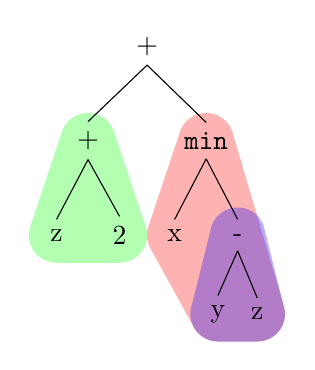
\begin{tikzpicture}[level distance=12mm,baseline=(current bounding box.center)]
\tikzstyle{level 1}=[sibling distance=15mm]
\tikzstyle{level 2}=[sibling distance=8mm]
\tikzstyle{level 3}=[level distance=10mm,sibling distance=5mm]

% tried to label subtrees but positioning looks weird, fix later
\node (+) {+}
  child { node (+2) {+}
    child { node (z) {z}  } % edge from parent node[left,draw=none] {$v_1$}
    child { node (2) {2} }}
  child { node (min) {\hmin}
    child { node (x) {x}}
    child { node (-) {-} %edge from parent node[right,draw=none] {$v_2$}
      child {node (y) {y}}
      child {node (z1) {z} } % edge from parent node[right,draw=none] {$v_3$}}
    }};


\begin{pgfonlayer}{background}
\fill[red,opacity=0.3] \convexpath{x, min, z1, y}{10pt};
\fill[blue,opacity=0.3] \convexpath{y, -, z1}{10pt};
\fill[green,opacity=0.3] \convexpath{z, +2, 2}{10pt};
\end{pgfonlayer}
\end{tikzpicture} &
\begin{tabular}{llll}
$(z + 2) + \hmin(x, y - z)$ & $\hmin(x, y - z)$ & $z + 2$ & $y - z$ \\
$v_1 + \hmin(x, y - z)$ & $\hmin(x, v_2)$ & & \\
$v_1 + \hmin(x, v_3)$ & & & \\
$(z + 2) + \hmin(x, v_3)$ & & & \\
$v_1 + v_2$ & & &
\end{tabular}
\end{tabular}
\caption{Given the input expression $(z + 2) + \hmin(x, y - z)$, we find all possible 
LHS patterns by substituting fresh variables for subterms, for all valid combinations. Then, we repeat the process for 
each individual subterm. This process yields the list of candidate LHS terms on the right.}
\label{fig:lhspatterns}
\end{figure*}

\subsection{Generating LHS Patterns}

  Our first step is to find LHS terms that could match the input expression, or any portion of it. 
We can enumerate all such terms through a kind of inverse matching.
When we rewrite an expression with a rule, 
we match the expression to the rule's LHS by finding a substitution for all variables in
the LHS that will unify it with the input expression. Here, we start with an input expression,
then fix a substitution by mapping some of its subterms to fresh variables. We 
replace those subterms with the new variables, constructing a term that can 
be matched with the input term.
If we perform this inverse matching for all sets of subterms, we find \emph{all possible LHSs} that could match the
input expression. 
When a subterm occurs more than once in the input expression, we construct a LHS that 
uses the same variable to replace it in multiple places and LHSs that replace its
occurrences with different variables.
We repeat the procedure on all \emph{subterms} of the input expression.  The result is the set of all 
LHSs that match any part of the input expression. See Figure~\ref{fig:lhspatterns} for a worked example.

This number of LHSs is exponential in the size of the input expression, so we use a few heuristics to narrow 
our search. We bound the size of candidate LHSs to have seven or fewer leaves, since longer terms are less likely to 
result in rules general enough to justify inclusion in the ruleset. 
Additionally, since we process input expressions in batches, we remove 
duplicate LHSs as well as LHSs that differ only in the values of their constants. 
Finally, we have found it helpful to keep a blacklist of LHSs for which we previously
failed synthesize rules; for example, $v_1 + v_3$ 
cannot form a rule, so we filter it out as a candidate.

\subsection{Synthesizing Right-Hand Sides} 
\label{sec:synthesizing-candidate-rules}
%
Given a candidate left-hand side, we attempt to 
synthesize a right-hand side that is semantically equivalent and
respects the reduction order, namely $\mathit{LHS} > \mathit{RHS}$.
We employ two strategies for synthesizing right-hand sides:
delayed AC matching, and counter-example guided inductive synthesis (CEGIS) of 
the RHS followed by synthesis of the rule predicate guard.

\subsubsection{Finding Right-Hand Sides through AC Matching}
\label{sec:rhsacmatching}
The first strategy reflects the Halide design decision not to perform any AC matching in the TRS, for efficiency reasons. 
Instead, AC matching is effectively performed during rule synthesis, by checking whether the LHS could be 
rewritten by the existing TRS after a suitable application of associativity and commutativity laws to the LHS. 
To this end, we generate all possible reassociations and commutations of the candidate LHS term and pass them to the existing TRS. 
If any of them can be simplified, we create a new rule that rewrites 
the original, untransformed LHS term to the result of the simplification.  Note that this result may include applications of more than one rewriting step, so the new rule is not merely an AC-variant of an existing rule.

For example, assume our TRS includes the rule $(x + y) - x \rewrites y$, 
and let $((u + 2) + v) - u$ be a candidate LHS term. The rule does not match the candidate but it matches its variant $(u + (v + 2)) - u$, rewriting it to the result $v + 2$. The candidate and the result give us the rule $((u + 2) + v) - u \rewrites v + 2$.

We can consider this procedure a kind of lazy offline AC matching, because if the Halide TRS 
performed full AC matching while rewriting expressions, it would be able to apply the rule $(x + y) - x \rewrites  y$ to the candidate expression $((u + 2) + v) - u$ after reassociating it to $(u + (v + 2)) - u$, obtaining the result $v + 2$.  Delaying AC matching to synthesis has the effect of restricting the system to a single, offline round of AC and memoizing the result in the form of a new TRS rule if we are successful. 
Note that the synthesis procedure below could have found this rule, but checking for AC
variants of existing rules is far cheaper. About three-quarters of our synthesized rules are generated by this method.

\subsubsection{Finding Right-Hand Sides through CEGIS}
\label{sec:rhssynthesis}
If the first method fails, we apply counterexample guided inductive synthesis (CEGIS)~\cite{DBLP:conf/aplas/Solar-Lezama09} to superoptimize the left-hand side pattern.
In superoptimization~\cite{massalin1987superoptimizer}, we take a program and search 
for an equivalent program within some grammar that is preferable according 
to some cost function. Here our grammar is that of the Halide expression language, 
the method for testing program equivalence is the Z3 solver, and we use the node
count of the programs as a proxy for our full reduction order.

Similar to prior work in superoptimization~\cite{regehr2018superoptimization, mangpo2016superoptimization},
we search the expression space for an equivalent RHS using a CEGIS loop. This loop alternately calls Z3 as a
verifier, which checks if a candidate RHS is equivalent to the LHS on all inputs, 
and a learner, which finds a candidate RHS that is equivalent to the LHS on
a limited set of inputs.
We begin by choosing a single-op
RHS and ask the verifier if it is equivalent to the LHS. If it is not, we get back 
a counterexample of assignments to the variables for which the right- and left-hand side are 
not equivalent, which we keep as a set of test inputs. 
We then ask the learner for a new RHS that is equivalent to the LHS 
only on the counterexample assignments we found in the last step. 
If we cannot find an equivalent single-op sequence,
we iteratively increase the number of operations, ensuring we find shorter sequences
first.  If CEGIS returns a sequence semantically equivalent to the LHS pattern with fewer
operations, we use it together with our LHS to form a candidate rule.

 The learner portion of the CEGIS loop creates a candidate RHS
  %expression from a parameterized bytecode
  %sequence of fixed size that is fed to an interpreter. Each bytecode
  %instruction takes parameters that select between the possible operators and
  %operands available to it. Thus,
  %this bytecode
  %sequence serves as an SSA representation of an expression tree. The
  %interpreter is evaluated abstractly on symbolic inputs to produce a
  %sketch~\cite{DBLP:conf/aplas/Solar-Lezama09, torlak2014lightweight}, 
  %capable of acting as any Halide expression in our
  %search space depending on the bytecode values. The learner uses Z3
  by creating a sketch~\cite{DBLP:conf/aplas/Solar-Lezama09, torlak2014lightweight}
  that consists of a small bytecode interpreter that encodes the possible
  operations and operands the RHS can use, along with a bound on the number of instructions.
  The learner uses Z3 to query for a sequence of bytecodes within the bound, that, when
  run through the interpreter, is semantically
  %solve for the bytecode values that makes the sketch semantically
  equivalent to the LHS over the test inputs. If a solution is found,
  substituting the produced bytecode values into the sketch
  and applying the TRS reduces it to a concrete candidate RHS. One
  complication arising from this approach is that a bytecode sequence
  of a fixed number of ops may produce expression trees of a larger
  size if intermediate values are reused. We reject any such solutions
  in a post-pass by checking each synthesized RHS against the LHS
  using the full reduction order. An alternative solution would be
  introducing let bindings into our search space so that the size of
  the expression tree could be bounded by the number of ops in its SSA
  form. However, we could not identify any significant rewrite rules
  lost to this filtering, so we deemed this an unnecessary
  complication. 

While Z3 is a powerful tool for synthesis, there are certain types of expressions 
containing division or modulo that Z3 nearly always fails to reason about during the CEGIS process. (We experimented with the SMT solvers Yices2~\cite{jovanovic2017solving} and MathSAT5~\cite{mathsat5}, but were not able to obtain appreciably better results.)
Z3 is better able to reason about expressions containing concrete constants, rather than
universally quantified variables, so we synthesize rules using candidate LHSs with 
concrete constants from the input expression and generalize them later.
We limit the use of division and modulo in our op-codes to be division
or modulo by 2 only, and rely on the generalization step described next to
widen the set of denominators for which a rule applies.  Because of this
restriction, our synthesized rules cannot contain non-constants in denominators
or the right-hand side of a modulo.  As a result, our synthesis system cannot
construct all rules a human can.

\begin{table*}
\caption{Sample rules synthesized by our process. }
\small
\begin{tabular}{l|l|l}
LHS & RHS & Predicate \\
\hline
$(x*y) - (z + (w*x))$ & $(x*(y - w)) - z $ & \\
$x < (y + x) + z$ &  $0 < (y + z)$ & \\
$\hmax(x*x, y) + \hmax(z, w*w) < c_0$ & false & $c_0 <= 0$ \\
$\hsel(x, c_0, y) < \hmin(\hsel(x, c_1, y), c_2)$ & false & $\hmin(c_1, c_2) <= c_0$ \\
$\hmin((x + ((y - x)/c_0)*c_0) + c_1, y)$ & $y$ & $1 <= c_1 \wedge -1 <= (-1/c_0)*c_0 + c_1$ \\
\end{tabular}
\label{tab:samplerules}
\end{table*}

\subsection{Generalizing Constants and Finding Predicate Guards}
\label{sec:generalizing-constants}

If either AC-matching search (Section~\ref{sec:rhsacmatching}) or CEGIS-based synthesis (Section~\ref{sec:rhssynthesis}) were successful, 
we now have a candidate rewrite
rule that contains concrete values originating from the input expression.
To generalize the rule, we replace such constants with fresh \emph{symbolic constants} 
and synthesize a guard that is true when the rule is valid. 
Recall that in the Halide TRS, a variable in the LHS matches any subterm, while a 
symbolic constant matches only a constant value (see Section~\ref{sec:customalgo}); the guards, which are predicates over symbolic constants, can thus be evaluated at compile time. 

Our goal is to generalize the equality by synthesizing a guard predicate $\phi$ 
over the symbolic constants in the LHS and RHS terms such that our rule is valid whenever
$\phi$ evaluates to true:
\[ \forall \vec{c} \forall \vec{x} \;.\; \phi(\vec{c}) \implies LHS(\vec{x},\vec{c}) = RHS(\vec{x},\vec{c})
\]

First, we check to see if this condition is satisfied when $\phi$ is 
always true. If it is, then no predicate guard is needed. Otherwise, we need 
to synthesize an expression for $\phi$. We find candidates for $\phi$ iteratively 
by first choosing a small set of values $S$ for the variables 
in $\vec{x}$ and finding the candidate guard $\phi_S$. We check to see if $\phi_S$
is a sufficient predicate guard for all $\vec{x}$; if it is not, we add
counterexamples to the set $S$ and repeat.

\[ \forall \vec{c} \forall \vec{x} \in S \;.\; \phi_S(\vec{c}) \implies LHS(\vec{x},\vec{c}) = RHS(\vec{x},\vec{c})
\]

We initialize $S$ with all basis vectors, which are 
values $\vec{x} = ( 0, \ldots, 0, 1, 0, \ldots, 0 )$ that include exactly one unit value,
plus the zero vector.  
We then unwind the right-hand side of the implication and substitute in the concrete values 
from $S$ to get:

\[ \forall \vec{c} \forall \vec{x} \in S \;.\; \phi_S(\vec{c}) \implies (LHS(\vec{x_1},\vec{c}) = RHS(\vec{x_1},\vec{c}) \wedge \ldots \wedge
LHS(\vec{x_k},\vec{c}) = RHS(\vec{x_k},\vec{c}))
\]

We use the Halide TRS itself to simplify the conjunction on the right-hand side of the
implication. Since all occurrences of $\vec{x}$ have been replaced with concrete
values, we get back an expression that contains only symbolic constants, which we
use as our candidate guard $\phi_S$.

We test whether $\phi_S$ is sound on all $\vec{x}$.
\[ \exists \vec{c} \; \exists \vec{x} 
   \;.\; LHS(\vec{x},\vec{c}) \not= RHS(\vec{x},\vec{c})
\]

If this query has a solution $\vec{x}$, then the guard is unsound.  
If so, we add the counterexample $\vec{x}$ to $S$, and construct a new guard $\phi_S$.  
We repeat this process for several iterations (four, in our experiments) and if 
we fail to find a sound guard, we switch to an alternative strategy that converts 
the current (unsound) candidate $\phi_S$ to disjunctive normal form and tests
each clause in turn to check if it is a sufficient guard.
If it is, that clause becomes the guard.  If no clause is sound, we discard the rule.
If the loop terminates with Z3 timing out or returning ``unknown'', we return
the current $\phi_S$, flagging it as requiring a manual proof. 
We exclude all such cases from our experiments.


As an example, consider the candidate rule:
%
\[ x_0 < \hsel(x_1, c_0, c_1) + x_0 \rewrites \neg x_1
\]
We initialize $S$ with three basis vectors $\{(0,\mathit{false}), (0,\mathit{true}), (1,\mathit{false})\}$ and construct $\phi_S$:
%
\begin{equation*}
\begin{split}
 \phi_S(\vec{c}) \iff 
 &  \forall_{\vec{x} \in S} \;.\; LHS(\vec{x},\vec{c}) = RHS(\vec{x},\vec{c}) \\
 \iff & 
 0 < \hsel(\mathit{false}, c_0, c_1) + 0 = \neg\mathit{false} \; \wedge \\
                                                   & 0 < \hsel(\mathit{true}, c_0, c_1) + 0 = \neg \mathit{true}  \; \wedge \\
                                                   & 1 < \hsel(\mathit{false}, c_0, c_1) + 1 = \neg\mathit{false}
\end{split}
\end{equation*}

Simplifying the RHS with the TRS, we obtain $\phi_S$:
%
\[  \phi_S(\vec{c}) \iff 0 < c_1 \wedge c_0 \le 0
\]

Next we check whether $\phi_S$ is sound for all $\vec{x}$.  It is, so we have a completed rule:

\[ x_0 < \hsel(x_1, c_0, c_1) + x_0) \rewrites \neg x_1 \;\pred \;0 < c_1 \wedge c_0 \le 0
\]


\subsection{Adding Rule Variants}
\label{sec:rulevariants}
Once we have a generalized rule with a valid predicate, we eagerly compensate for the lack
of AC matching in the Halide TRS by adding AC variants of the rule as well. We find 
all commuted variants of the rule's LHS,
with respect to the partial commutative canonicalization as described in Section~\ref{sec:customalgo}.
 (This is exponential in the size of the number 
of commutative operators, which is tractable given our bounds on LHS term size). 
Then, we find all reassociations of the rule's right-hand side. For each variant LHS, 
we choose a RHS variant by serializing expressions to strings and finding the RHS 
that has the shortest edit distance from that LHS.

For example, the LHS of the first rule below has four additions and can be commuted 
to 16 variants. The RHS of the rule can be reassociated in two different ways. For the 
commuted variant of the LHS on the second line, we choose the other means of reassociating
the RHS as it has a smaller edit distance.

\begin{equation*}
\begin{split}
(x + (y - ((z + (w + x)) + u))) & \rewrites y - (z + (w + u))) \\
(y - (((w + x) + z) + u)) + x & \rewrites y - ((z + w) + u)
\end{split}
\end{equation*}

The intuition is that there is no a priori reason 
to prefer one reassociated variant to another; they are almost certainly equal in 
terms of our reduction order. Thus, we choose the RHS that perturbs the structure of the 
LHS as little as possible, in order to avoid rewriting common subexpressions in the hopes
of canceling them out later.


\subsection{Filtering Rule Output}
\label{sec:filtering}
As a final step, we check each output rule for redundancy with the rule batch found
by the synthesis pipeline. For each new rule, we check
that no earlier rule has precisely the same LHS and predicate; if so, it can be discarded.
Then, we check that no earlier rule is more general than the current rule: a rule is more 
general than another if they have similar LHSs, but a variable appears in the first rule 
in a place where the second rule has a more specific subterm, or if they have the same LHS
but the predicate of the first rule implies the predicate of the second.

Finally, we
check that the candidate rule obeys our reduction order in order to
preserve our termination guarantee. If the candidate rule passes these
filters, and the predicate has not been flagged for human review, the
rule can be added to the TRS ruleset automatically without any human
auditing.

\section{Evaluation of Simplifier TRS Synthesis}

\section{Evaluation}
\label{sec:evaluation}

% (1186-367)/1186
\newcommand{\PercentPossibleToSynth}{69\%}
\newcommand{\NumRulesInCorrectnessExperiment}{321}
\newcommand{\PercentRulesResynthesized}{58\%}

In evaluating the benefits of the verifier and synthesizer, we answer the following questions:

\begin{itemize}
  \item \textbf{Does the synthesizer produce better rules than a human expert?} The TRS has been manually extended five times in response to bug reports pointing out limitations of the compiler. We synthesized these five rulesets automatically and found that the human-authored rules were less general and in one case were incorrect. (Section~\ref{sub:bugfixes})
 
  \item \textbf{What is the best way to use synthesis and verification in development?} We survey several cases from recent Halide development where human experts used the synthesis machinery as an assistant, finding that this hybrid model is more powerful than either the human developer or the synthesizer alone. (Section~\ref{sub:synthassistant})
  \item \textbf{Can synthesis be used for large-scale improvements of the TRS?} We gather a corpus of over 100,000 expressions on which the TRS can make no progress and iteratively synthesize rules using the corpus as input. We synthesize \NumRulesSynthesized  rules and add them to the TRS ruleset without a human audit. We find that the enhanced ruleset reduces peak memory usage in compiled code, sometimes dramatically, in 197 of our benchmarks. We also find no significant compile-time slowdown even with this 4.5-fold increase in ruleset size. (Section~\ref{sub:endtoendexperiment})
  \item \textbf{Could the entire TRS have been synthesized?} Encouraged by the large-scale experiment, we ask how far we are from being able to bootstrap the entire TRS automatically---something that we considered too ambitious originally. First, we find that \PercentPossibleToSynth~of the existing ruleset is accessible to our current synthesizer in principle; the remaining rules contain operators not yet supported by the tool. % or cannot be reasoned about automatically by our solver. 
  We test the synthesizer's power by removing \NumRulesInCorrectnessExperiment{} accessible rules from the original ruleset one by one and attempting to synthesize a replacement, successfully finding a replacement rule \PercentRulesResynthesized{} of the time.  We find this encouraging for future applications of the synthesizer. (Section~\ref{sub:replacementexperiment})
\end{itemize}

We discuss these findings in more detail below, grouping them into three sections. First we examine bug reports from Halide’s past and evaluate whether the machinery presented in this paper could have fixed them automatically. Second, we examine cases where beta versions of our verifier and synthesizer assisted humans both in fixing bugs and in correctly making larger changes to the compiler. Third, we fuzz the compiler to mine for issues that could be fixed with new simplifier rules, and automatically fix them before they ever appear as a bug in a real program. In this way we demonstrate that this machinery would have been useful in the past, is useful in the present, and will help avoid entire classes of bugs in the future.

%\jln{don't forget to do this!}
%Note for reviewers: For the purposes of this anonymous submission, we will refer to code changes by letter, with corresponding diffs found in supplemental material. In this final version of the paper these will be replaced with GitHub issue and pull request IDs with links to Halide’s GitHub page.

\subsection{Comparing the Synthesizer to Human-Authored Rules}

\subsubsection{Does the Synthesizer Produce Better Rules than a Human Expert?}
\label{sub:bugfixes}

%We expect a human expert to create rules that are as general as possible while also including rules that take advantage of less general situations, such as when special cases allow stronger rewrites.  Can a synthesizer produce rules that are both general and expressive? 

%We compared synthesized rules against five sets of rules added manually. We have found that the expert wrote rules that were less general than the synthesized rules, and in some cases were incorrect. Additionally, the synthesizer avoided adding a specialized rule because the TRS could already achieve its effect with rules present in the TRS. We discuss in Section~\ref{sec:limitations} the limitations of when the synthesizer cannot achieve such general rules. 

% AA: I found the two paragraphs above redundant with the summary we just gave in the itemized list.


% A) https://github.com/halide/Halide/pull/3719
% B) https://github.com/halide/Halide/pull/3761
% C) https://github.com/halide/Halide/pull/3765
% D) https://github.com/halide/Halide/pull/3770
% E) https://github.com/halide/Halide/pull/3780
% F) https://github.com/halide/Halide/pull/4721
% G) https://github.com/halide/Halide/pull/4772
% H) https://github.com/halide/Halide/pull/4439
% I) https://github.com/halide/Halide/pull/4850 


We searched through Halide’s change history and selected the five pull requests that addressed issues by adding new rewrite rules to Halide’s TRS. These pull requests occurred before the Halide developers started routinely using the verifier and synthesizer when changing the TRS. These can be found as summarized diffs $\mathbb{A}$-$\mathbb{E}$ in supplemental material, or in their original form on the Halide project website
\footnote{
$\mathbb{A}$: \url{https://github.com/halide/Halide/pull/3719}
$\mathbb{B}$: \url{https://github.com/halide/Halide/pull/3761}
$\mathbb{C}$: \url{https://github.com/halide/Halide/pull/3765}
$\mathbb{D}$: \url{https://github.com/halide/Halide/pull/3770}
$\mathbb{E}$: \url{https://github.com/halide/Halide/pull/3780}
}.
Creating these rewrite rules as a human is an amount of work disproportionate to the size of the change. The author of the rules must prove them correct on paper, and a second reviewer must check their work. As we will see, bugs can slip through despite this review. 

In each case we take the test expressions committed as part of the change and feed them to our synthesizer to see if it would have produced the same rewrite rules as the humans did. In cases where humans did not check in tests for their new rules, we wrote our own. In total, across these five cases humans added 24 new rules. The synthesizer generated 42, covering all but one of the human rules, while correcting and generalizing others. In cases $\mathbb{A}$, $\mathbb{C}$, and $\mathbb{E}$, the rules generated by the synthesizer are an exact match to the human-generated rules. In case $\mathbb{B}$ the synthesizer matched the human but also crafted 8 commuted variants of the human rules, making them more widely applicable. 
\newpage
As an example, for the human-written rule:

\[
\hmax(\hmax(x, y) + c_0, x) \rewrites \hmax(x, y + c_0) \pred c_0 < 0
\]

The synthesizer produced effectively the same rule, along with a variant:

\begin{align*}
& \hmax((\hmax(x, y) + c_0), x) \rewrites \hmax((y + c_0), x) \pred c_0 \leq 0 \\
& \hmax(x, (\hmax(x, y) + c_0)) \rewrites \hmax(x, (y + c_0)) \pred c_0 \leq 0
\end{align*}

Case $\mathbb{D}$ is the most interesting. It contains four rules involving comparisons of $\hmin$ and $\hmax$ operations. What happened for each was identical, so we will only discuss the $\hmin$ rules. The first rule is:

\[
\hmin(x, c_0) < \hmin(x, c_1) + c_2 \rewrites \hfalse \pred c_0 \geq c_1 + c_2)
\]

This rule is incorrect (consider $c_0 = c_2 = 1$, $x = c_1 = 0$). It can be fixed by adding the term $c_2 \leq 0$ to the predicate. The synthesizer produced the correct version of this rule, along with two generalizations of it:

\begin{align*}
& \hmin(x, c_0) < \hmin(x, c_1) + c_2 \rewrites  \hfalse \pred c_2 \leq 0 \wedge c_1 + c_2 \leq c_0 \\
& \hmin(x, c_0) < \hmin(x, y) + c_1 \rewrites c_0 - c_1 < \hmin(x, y) \pred c_1 \leq 0 \\
& \hmin(x, c_0) < \hmin(y, x) + c_1 \rewrites c_0 - c_1 < \hmin(y, x) \pred c_1 \leq 0
\end{align*}

The second human rule was:
\[
\hmin(x, c_0) < \hmin(x, c_1) \rewrites \hfalse \pred c_0 \geq c_1
\]
The synthesizer found a more general rule, along with three other commuted variants (elided for space):
\[
\hmin(x, y) < \hmin(x, z) \rewrites y < \hmin(x, z)
\]
Any expression which matches the human-written rule would also match the synthesized one. The synthesized version does not simplify to the constant false in a single step. However, after applying this rule to the case considered by the human, we get $c_0 < \hmin(x, c_1)$ where $c_0 \geq c_1$. The simplifier then reduces this to false in a second step, so the human-written rule becomes unnecessary. The synthesizer considered the human-written rule, but discarded it as less general than the one above.

Case $\mathbb{D}$ also included the rewrite rule: 
\[
x\; \%\; x \rewrites 0
\]
which was the sole rule the synthesizer could not generate, as we did not include modulo by non-constants in our CEGIS interpreter.

With this one exception, across these five code changes the synthesizer generated more general, more correct rules than the humans, and would clearly have been a useful assistant to the Halide developers if they had had it at the time.


\subsubsection{What Fraction of the Halide Rules Could Have Been Synthesized?}
\label{sub:replacementexperiment}
To bootstrap a TRS, we could start with a TRS equipped with a basic set of rules and synthesize the remaining rules as the TRS encounters expressions needing those rules.  How far is the synthesizer from supporting this ambitious vision?

Given the space of possible rewrites explored by the synthesizer, we believe that it can currently produce at most \PercentPossibleToSynth{} of rules that exist in the current TRS. The obstacles to synthesizing all human-written rules include (i)~the inability to automatically verify some rules or preconditions (see Question 3 above); and (ii)~lack of support for some operators in our synthesizer. 

We tested the synthesizer's ability to recreate the original ruleset in the following experiment. We instrumented the ruleset to associate expressions from compilations of Halide's correctness test suite with individual rules invoked when those expressions are rewritten. We gathered a set of rules for which we had at least three expressions that matched the rule, and filtered out those rules that are out of scope for the current synthesizer, because their right-hand sides contain operators we do not support. This gave us a set of \NumRulesInCorrectnessExperiment{} rules. For each of these rules, we disabled the rule in the TRS, then used its matching expressions as input to the synthesizer. The synthesizer was able to find rules in 186 cases, or about \PercentRulesResynthesized{} of the rules. Of the other 135 cases, in 43 of them other rules in the existing TRS happened to combine to rewrite the specific input expression even without the target rule; for example, this often occurred when the matching expression contained combinations of constants that could be exploited by other rules. 10 of the 92 failure cases were due to timeouts in the synthesis process, while 15 specifically failed to synthesize a predicate. Given that it was difficult to target the desired rule precisely, we find these results to be a promising state of the technology.


\subsection{Practical Uses of the Synthesizer and Verifier}





\subsubsection{What is the Best Way to Use Synthesis and Verification in Development?}
\label{sub:synthassistant}

% Is the expert equipped with the synthesizer better at developing rules than either the expert alone or the synthesizer alone? The synthesizer can accelerate rule development because it is correct by construction and also faster than a human expert. On average, the expert needed about 30 minutes to develop a rule, including a paper proof and the code review. Our synthesizer typically produces a batch of ten (verified) rules in about 5 minutes.

We have found that human experts can best leverage the strengths of the synthesis tool by using it as an assistant: for example by synthesizing a rule and then generalizing or simplifying it by hand, or by writing a rule and asking the tool to synthesize a valid predicate. Most importantly, this avoids committing new bugs, but it also accelerates rule development. Halide developers report that adding new rules by hand takes about 30 minutes per rule starting from sample input expressions through final review. Starting from the same input expressions, the synthesis tool can produce a batch of 10 verified rules in about 5 minutes.

Here we survey some cases from recent Halide development where the synthesis machinery was used in this way. The diffs are available as $\mathbb{F}$ through $\mathbb{I}$ in supplemental material or on the Halide project website\textsuperscript{\ref{footnote:casesfi}}.

In case $\mathbb{F}$ a Halide developer encountered expressions that seemed like they could be simpler while working on real code, and rather than inventing a rule from scratch searched the logs of the synthesizer project for a known-correct synthesized rule that handled the case in question. This added four new rules that are variants of:
\[
\hmax(y, z) < \hmin(x, y) \rewrites \mathit{false}
\]
In case $\mathbb{G}$ a developer wrote 24 new rules, proving them on paper, and then checked their work by resynthesizing the predicates using the synthesizer, ensuring that the synthesized predicates agreed with the human’s and that those predicates were as broad as possible. Here the synthesis machinery served as a reviewer of rules rather than an author. Eight of these rules were in fact manual rederivations of the synthesizer’s output on case $\mathbb{D}$ above. The remaining 16 are generalizations that add constant terms. One example:
\[
\hmin(y + c_0, z) < \hmin(y, x) \rewrites \hmin(z, y + c_0) < x \pred c_0 < 0
\]

Halide endeavors to be a safe language, meaning that certain things are checked at compile time or runtime rather than being undefined behavior. In case $\mathbb{I}$, Halide was changed such that instead of asserting that no output value has a dependency on any out-of-bounds input values, it now asserts the stricter condition that no out-of-bounds loads occur on the input, even if those loaded values cannot possibly affect an output.

This is a harder thing for the compiler to check, and analysis often conservatively found that it was possible for code to read out of bounds, when in fact it would not. The Halide developers ameliorate this in part by minimizing the number of non-monotonic expressions using aggressive simplification. In total 59 new rewrite rules were added as part of this change. Eight of these were synthesized automatically by copy-pasting a non-monotonic expression from a bug report into the synthesis machinery. Another 28 came from generalizing those rules by hand and then verifying the result. Twenty more were written by hand and then verified. Finally, there were three rules that could not be verified, because they involve the interaction of division and modulus. During this process a large number of bugs were found in human-written early versions of these rules. We found that with the verifier and synthesizer in hand, humans work quickly and rely on the machinery to catch their mistakes.

Generalizing from these four cases, we have found that having the verifier and synthesizer available as tools reduces the number of bugs committed, uncovers and fixes old bugs, and helps developers work more quickly by not only mechanizing correctness checking but also by synthesizing correct code. We also found that the guarantees these tools provide mean that the developers can make large changes to the compiler with confidence. Anecdotally, developers also report that eliminating these classes of bug makes triaging new issues simpler, because they could now not possibly be due to an incorrect rule or an infinite loop in the term rewriting system.

\subsection{Using the Synthesizer to Prevent Future Issues}
\label{ssec:compilationspeed}

\subsubsection{Can Synthesis be Used for Large-scale Improvements of the TRS?\nopunct}
\label{sub:endtoendexperiment}
%What improvements are possible when we allow the synthesizer to learn rules from a large body of input, without human supervision? In this experiment, rather than synthesizing a repair to just one incorrect rule, we attempted to synthesize rules for over 100,000 expressions that failed to simplify over thousands of instrumented compilations. We synthesized 4127 rules and added them to the TRS. In evaluating the effects of these improvements, we found 197 benchmarks that were over-allocating memory, sometimes dramatically, due to imprecise bounds reasoning caused by missing rules. Those benchmarks were fixed by the improved TRS. Synthesis allowed us to make this dramatic change to the ruleset without fear of introducing non-terminating behavior, since synthesized rules must satisfy the reduction order (see Section~\ref{sub:termination}). Satisfying this additional restriction would further complicate manual rule development. 

%% AA: I found the above paragraph redundant with the summary at the start of the section and the more detail version below. If we want an intro para here I think it should be shorter.

Although we now have a guarantee of soundness, we have no such guarantee of completeness. There are almost certainly Halide compilations for which the addition of some desirable rule would strengthen the TRS enough to unlock some optimization or achieve a tighter bound on some region. However, we don’t know what they are because no human has encountered them yet (or more likely, no human has been sufficiently motivated to submit a bug report for them yet). 

We attempted to probe for such opportunities for improvement using fuzzing. We selected the 12 most complex example applications in the open source repository, and generated 64 random schedules for each using the autoscheduler~\cite{Adams2019}, which can be configured to generate random likely-good schedules. This produced 768 separate compilations. We also instrumented most of the Halide code at Google for an additional 5032 compilations, this time using the original human-written schedules. Note that this is qualitatively different to randomly-generated schedules: we do not expect Halide users at Google would check in code that behaves poorly due to an issue with the compiler.

We instrumented these compilations to log expressions that might represent a TRS failure of some kind. From each compilation we log all integer expressions found that are non-monotonic with respect to a containing loop, and all failed proof attempts made during compilation. That is, we log all boolean expressions passed to the TRS in the hope that they will reduce to the constant true so that some optimization can correctly be performed. This resulted in a corpus of roughly one hundred thousand unique expressions.

Using this corpus as input, we synthesize new rewrite rules, add all rules found back to the ruleset, and rerun all compilations to gather new expressions, repeating this process until convergence. In total we created 4127 new rewrite rules in this way, more than quadrupling the number of rules in the TRS. For some examples, refer to Table \ref{tab:samplerules}.

We then generate a fresh set of 256 random schedules per application (to avoid testing on our training set), and compile and run all the generated code, looking for any compilations which behave significantly differently between the baseline condition (compiled using unmodified Halide) and the test condition (compiled with the 4127 additional rewrite rules). The interesting findings are summarized below.

\paragraph{Adding new rules lowers peak memory usage by up to 50\%}
Halide sizes internal allocations using symbolic interval arithmetic,
which (as described in Section~\ref{sec:synthesizing-candidate-rules})
is prone to overestimating bounds when
expressions do not either monotonically increase or decrease with
respect to some containing loop. By extending the TRS, we
automatically fix 197 cases where this kind of error increases the
peak memory usage of an application at runtime by more than 10\%, including one
case where the increase was more than a gigabyte. This represents
nearly 6\% of all compilations tested. We believe this captures a
widespread problem, as instances of overallocation are a common source
of complaint from users. See Figure~\ref{fig:peakmemoryhistogram} for
the full distribution. 

\begin{figure*}
  \includegraphics[width=4in]{figures/memoryhistogram.pdf}
\caption{Reduction in runtime peak memory usage of 3072 pieces of compiled
  code when 4127 synthesized rules are added to the TRS. The x-axis
  shows $\frac{after}{before}$, so below 1.0 means the synthesized rules
  reduced memory consumption.  In 197 cases,
  peak memory usage drops by more than 10\%.}
\label{fig:peakmemoryhistogram}
\end{figure*}

\paragraph{Term rewriting systems written without verification have bugs}
On our initial run of this experiment, 55 compilations (1.6\%) crashed
at runtime with memory corruption errors in the baseline condition (no
new rules added). We traced this to an incorrect transformation in a
separate, unverified TRS in the Halide compiler (the ``solver''). This
bug had existed for four years, but had only recently become an
important code path due to change $\mathbb{I}$ mentioned above. The
incorrect transformation was $\hmin(x - y, x - z) \rewrites x - \hmin(y, z)$,
which should be $\hmin(x - y, x - z) \rewrites x - \hmax(y, z)$. If this
secondary TRS had been written using verification, this bug would
never have been introduced. We intend to formalize and verify this
secondary TRS next to flush out any other bugs lurking therein.

\paragraph{The TRS scales well with the number of rules}
Remarkably, more than quadrupling the size of the TRS increased total compile
times by only 0.3\%. On further examination we found that the
additional rules increased the amount of time spent inside the TRS by
30\%, and that only 1\% of the the total compile time of the average
Halide program is spent inside the TRS.

We did not find significant effects on runtime of the generated code or code size. We also found no significant differences on any metrics within the Google corpus. This may be because the random schedules we generate are especially complex compared to human-written ones, or simply because humans don't commit code that causes the compiler to misbehave.

While adding this many new rules does not come at any significant cost we could measure to users of Halide, it increases the compile-time and code size of the compiler itself, so we do not propose adding all of these rules to the TRS permanently. Prior to proposing inclusion, we plan to triage the rules to select only those that are necessary to gain the peak memory reductions described above.

These results show that having verification and synthesis available as a tool for compiler authors fixes existing bugs, prevents entire classes of new bugs, and even helps compiler writers change the semantics of their language with confidence. We intend to continue to use verification and synthesis to maintain the TRS, and based on this experience plan to expand its use elsewhere in the compiler.

\section{Limitations \& Future Work}
\label{sec:limitations}
\jln{copied over from OOPSLA paper, but doesn't really belong here}
For this work, we considered only the subset of the term rewriting system that
is used to prove properties over infinite integers; the full TRS includes rules
for simplifying expressions with floating point values as well as rules for
fixed-bitwidth integers.  As a result, we do not consider cases where the TRS
must also reason about whether overflow can occur.  Extending our improvements
and automation to such rules could be done in future work.

One major limitation of the synthesis process we use is that our solver,
Z3, often cannot reason about expressions with divisions or modulo
where the right operand is a variable.  Though we work around this to
synthesize rules with generalized predicates on right hand side constants,
the overall synthesis machinery cannot generalize these to non-constants.
Extending the synthesizer may be more tractable for rules that operate
on integers with finite bitwidths.

The Halide TRS is used both to prove expressions true or false and to
simplify expressions to more easily optimizable forms, but these two use cases
are not always aligned. One could imagine two separate rewriters with
different rulesets and reduction orders. One interesting direction for future
work might be to use the synthesizer to create these two rulesets, which would
otherwise be a very human-effort intensive task.

Although we do not currently synthesize rules that contain vector operators,
they are not incompatible with our approach. Since our reduction of Halide
expressions to SMT2 formulas models vector expressions as integers, we would need
to add a typechecking step to ensure correctness in the synthesis process, which
we leave as future work.

The priority in which rules are considered for matching clearly can have
performance implications, but evaluation and tuning is left as future work, and
may require modifying our ordering or creating different orderings for different
uses of the term rewriting system.

Finally, while enhancing the Halide TRS was not able to improve the performance of the mature Halide compiler, we suspect this may not be the case for other, less well-exercised compiler backends. In future work we plan to use this technique to enhance the ruleset used to compile Halide applications to GPU code or to the Hexagon ISA.

\section{Synthesis for variable solver}

\begin{algorithm}[H]
\SetAlgoLined
\KwIn{goal function $\phi$, semantic equivalence relation $=_e$, reduction order $>$, set of training expressions $E$, set of test expressions $S$}
\KwResult{a term rewriting system $R$}
\While{$\exists s \in S \st \neg \phi(s)$}{
    choose $e \in E$, $l \in \texttt{lhs\_patterns(e)}$\;
        query synthesizer for $r$ such that $l =_e r \wedge l > r$\;
    \If{$r$ is found}{
        $R \gets  R \bigcup \;\{(l \rewrites r)\}$\;
        $E \gets \{ R(e) | e \in E \wedge \neg \phi(R(e))\}$\;
    }
}
\caption{Idealized procedure for synthesizing a term rewriting system}
\label{algo:synthesis}
\end{algorithm}

In our prior work, we synthesized individual rules to augment an already mature term rewriting system. In our proposed work, we plan to synthesize term rewriting systems from a small existing ruleset or completely from scratch. Our pipeline is sketched out below. In this section, we first justify the assumptions behind our approach. We then lay out our planned evaluation of our methodology on a new application, the variable solver term rewriting system within the Halide compiler.

An idealized version of our proposed synthesis procedure is laid out in algorithm~\ref{algo:synthesis}. This procedure requires a goal function, which returns true if a term is in some desired form and false otherwise; a semantic equivalence relation; and a reduction order over terms, as well of a set of training expressions $E$, which should be representative of the types of expressions the term rewriting system will take as input and a set of test expressions $S$ on which to evaluate the behavior of the term rewriting system.




\subsection{Rationale for synthesis pipeline}

Here we lay out the rationale for our proposed synthesis pipeline. In particular, we will discuss three key assumptions: that a reduction order can be an effective heuristic for guiding term rewrites to a desired form; that a term rewriting system can be synthesized as a series of individual rules; and that choosing candidate left-hand sides gathered from realistic inputs is an efficient means of finding rules that will have high impact on the performance of the term rewriting system.

When we specify a term rewriting system in this work, we say that it must have three properties:

\begin{itemize}
    \item it must be semantics-preserving
    \item it must terminate on all inputs
    \item it must rewrite terms into a form that has some desired property
\end{itemize}

In prior work, we showed that the Halide simplifier was semantics-preserving by verifying that for each rule $(l \rewrites r) \in R$, $l =_e r$, where the equality relation $=_e$ was checked by running the terms $l, r$ through an interpreter and sending the outputs to a solver to be checked. We showed that the TRS was terminating by choosing an order $>$ over terms and showing that every rule in $R$ rewrote terms to be strictly less in that order. When we synthesized new rules to add to the simplifier ruleset, we did not explicitly define the third criterion, but allowed the termination order fitted to the existing ruleset to guide the synthesis pipeline. 

In this section, we will define more precisely the goal or intent behind a term rewriting system. We argue that an effective means of specifying this intent for the purpose of synthesis is to use a reduction order to capture the notion of rewriting a term to be closer to some goal state.

\begin{figure}
    \centering
\subfigure[$\termlang$]{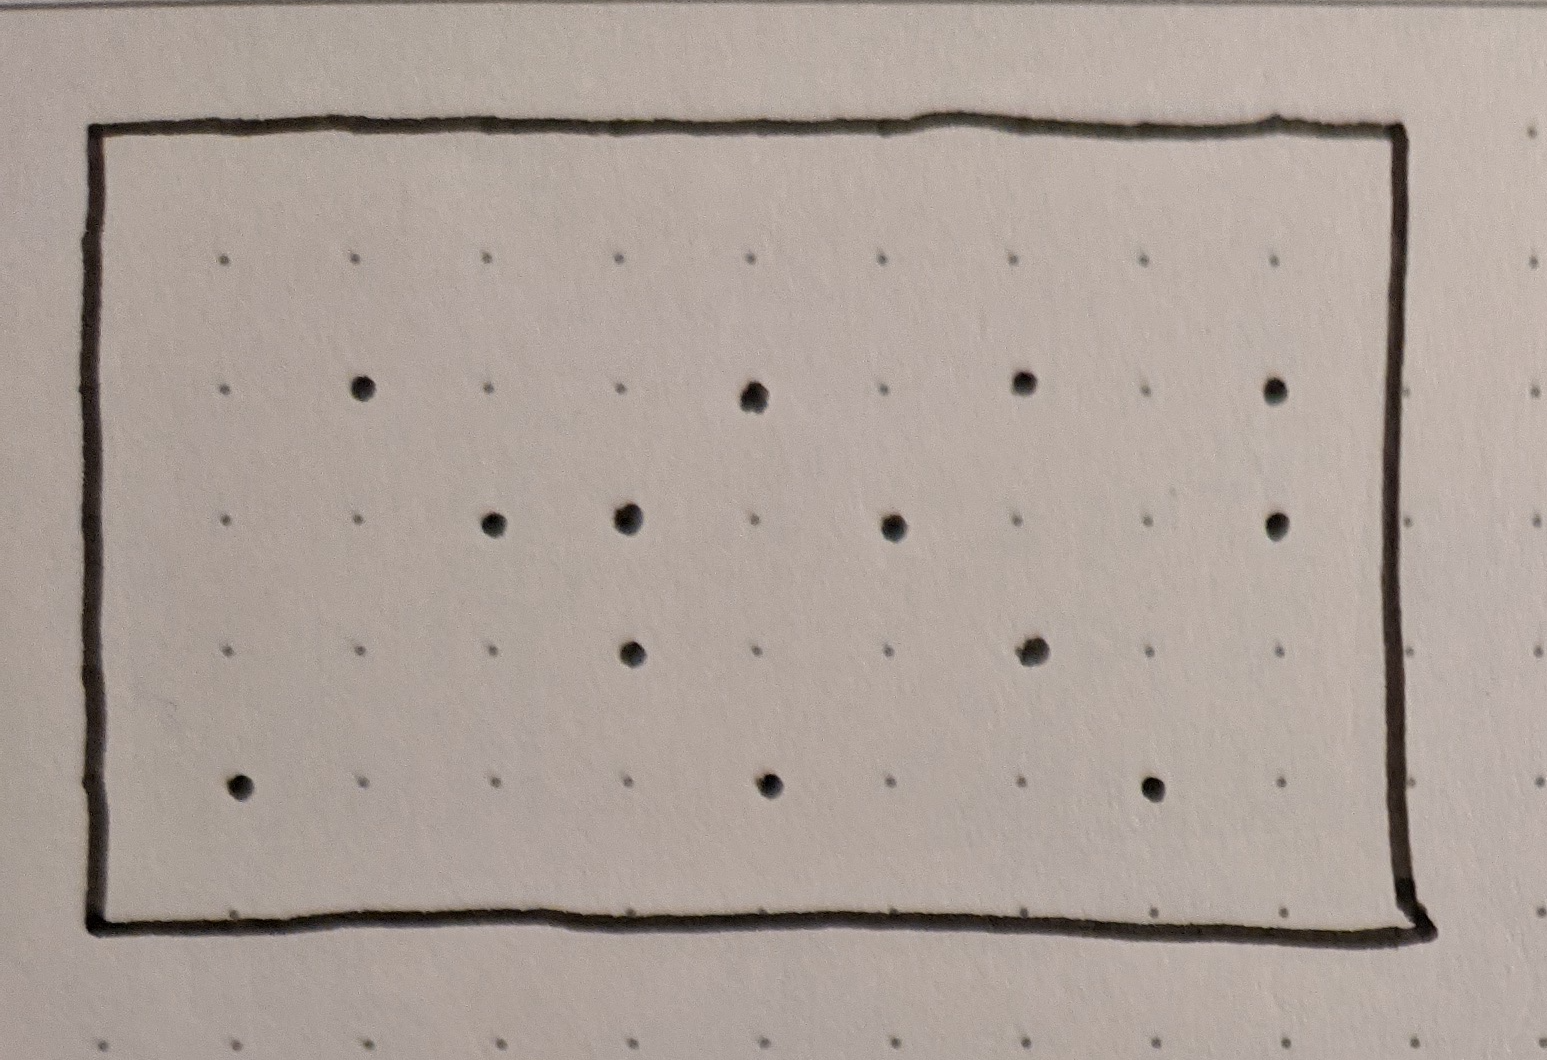
\includegraphics[width=0.3\textwidth]{figures/diagram1.png}}
    \hspace{1em}
    \subfigure[$\{s | s \in \termlang \wedge \phi(s)\}$ in red]{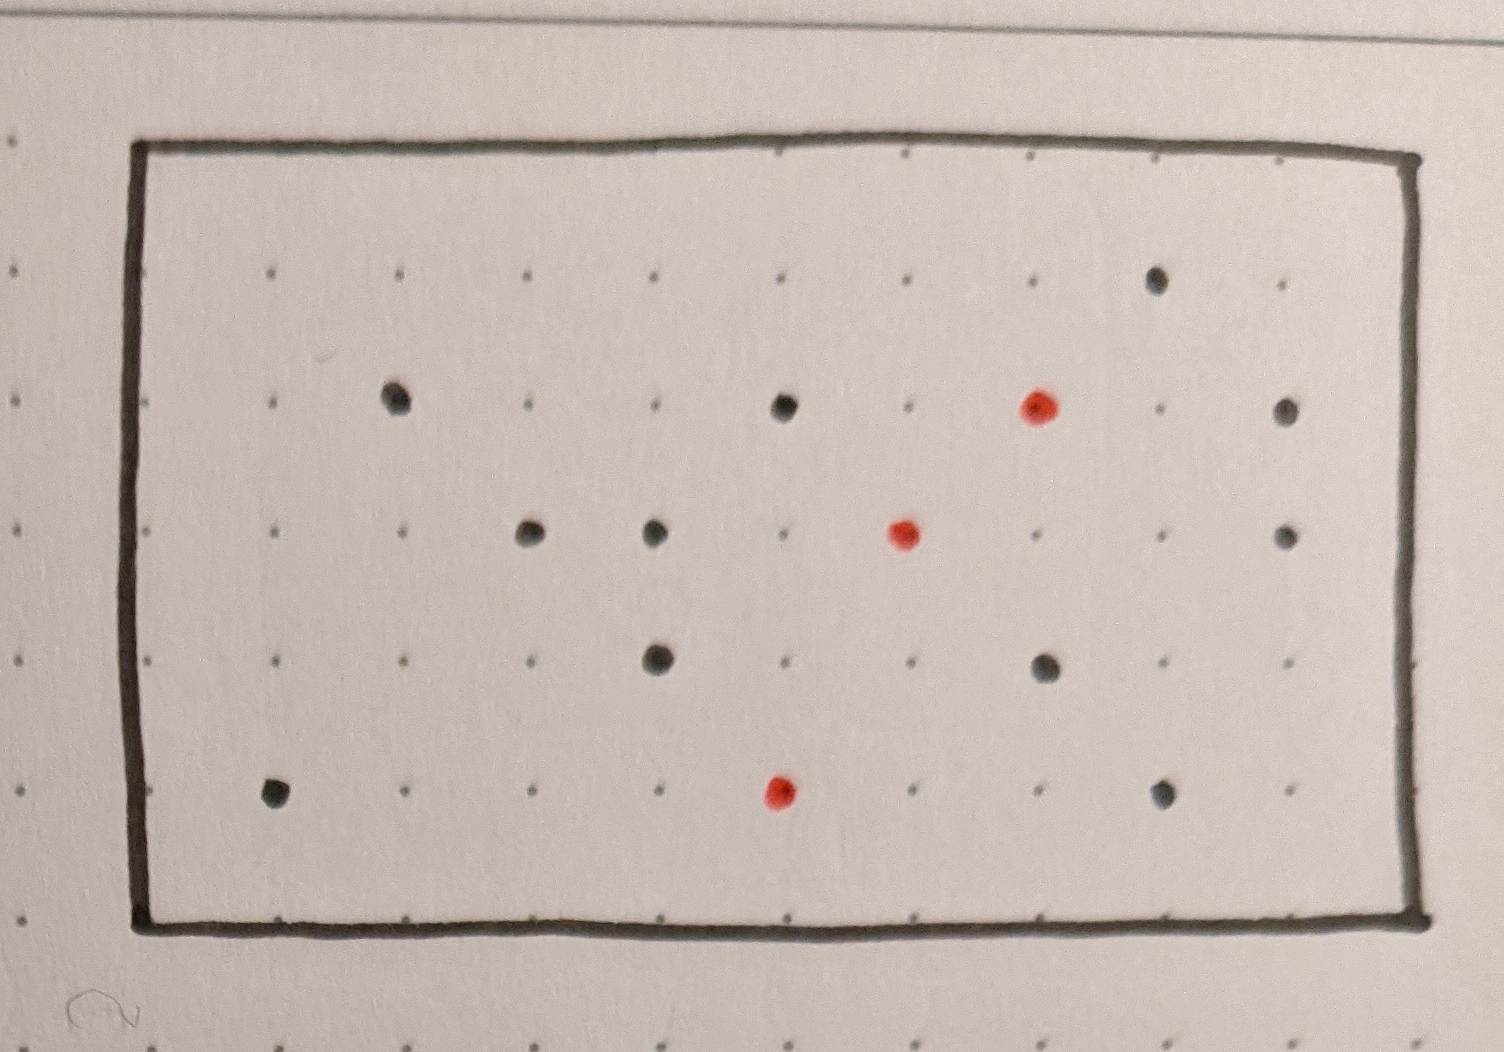
\includegraphics[width=0.3\textwidth]{figures/diagram2.png}}
    \hspace{1em}
    \subfigure[$\goallang$ in blue]{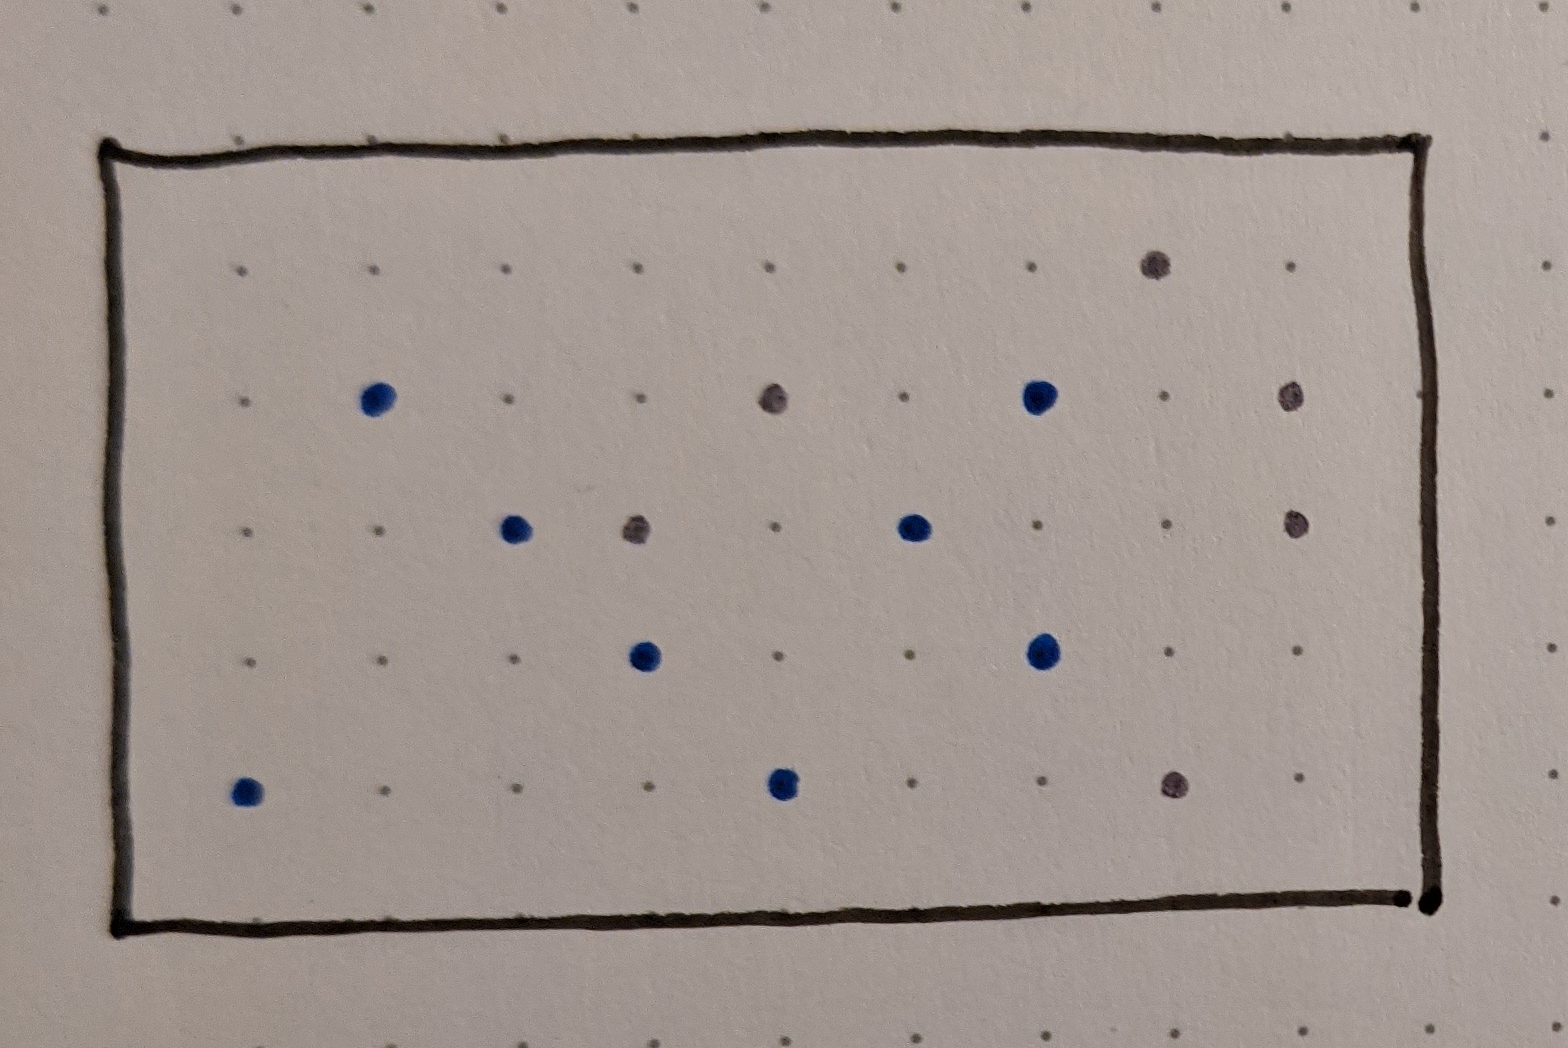
\includegraphics[width=0.3\textwidth]{figures/diagram3.png}} \\
    \subfigure[Undirected edges connect all $s, t$ st. $s =_e t$]{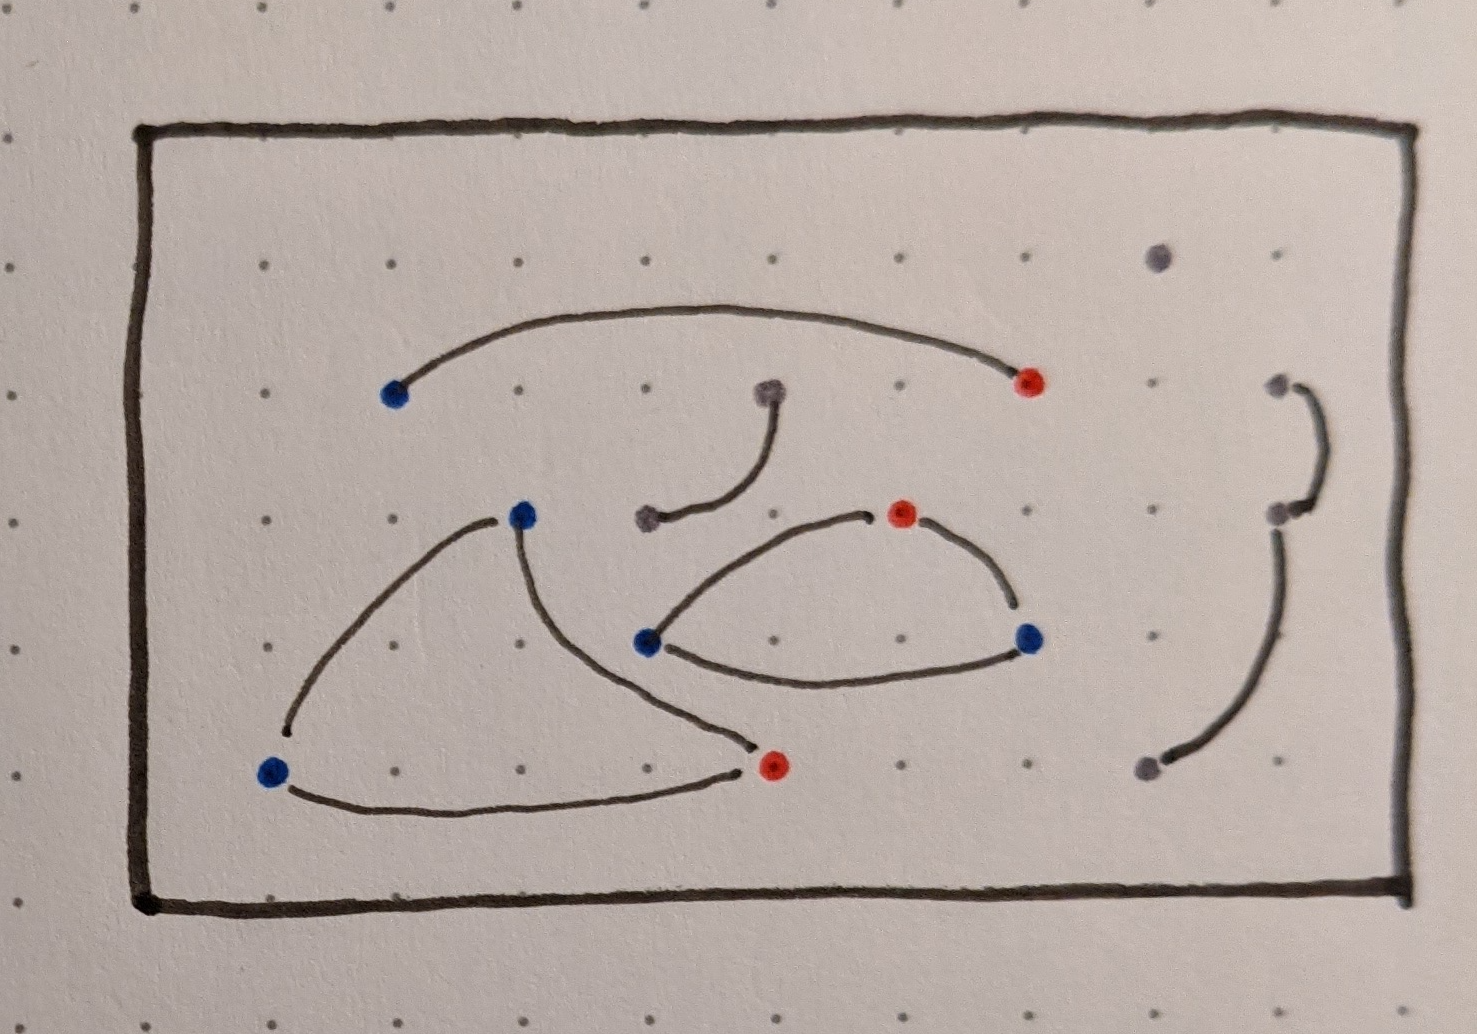
\includegraphics[width=0.3\textwidth]{figures/diagram4.png}}
    \hspace{1em}
    \subfigure[Directed edges connect all $s, t$ st. $s =_e t \wedge s > t$]{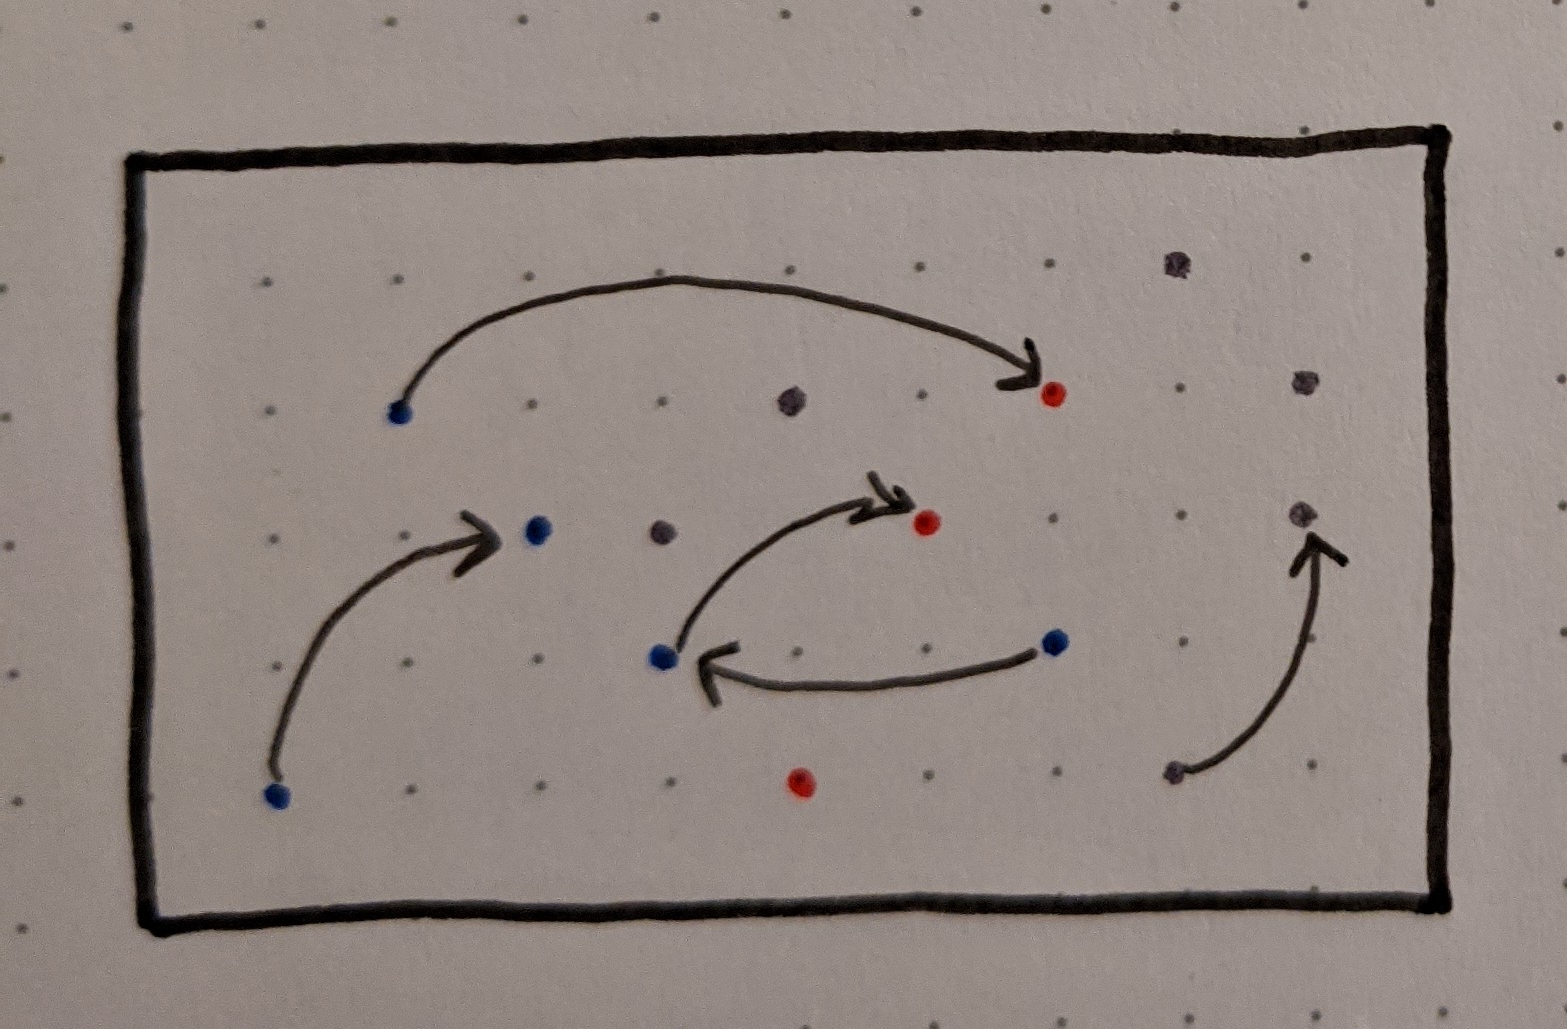
\includegraphics[width=0.3\textwidth]{figures/diagram5.png}}
    \caption{Each dot in (a) represents a term in $\termlang$. In (b), each term in the goal state is drawn in red. In (c), all terms which are equivalent to a term in the goal state ($\goallang$) are drawn in blue. The goal of the term rewriting system is to rewrite all blue dots in (c) to a red dot in (b). In (d), undirected edges connect all pairs of terms that are semantically equivalent. In (e), those edges have been oriented with a reduction order. Given the specification $\forall (l \rewrites r) \in R \st l =_e \wedge l > r$, we can find a TRS $R$ by picking a finite subset of all the directed edges in (e).}
    \label{fig:termuniverse}
\end{figure}

First, we define the goal property that describes the underlying intention of the term rewriting system. Assume some language of terms $\termlang$, a semantic equivalence relation over those terms $=_e$, and a syntactic equivalence relation $=$. We write the goal property as a predicate function $\phi$ such that $\phi(s)$ is true if $s$ is in the goal state and false otherwise. We can thus write the domain of the term rewriting system as a language $\goallang \subseteq \termlang$, defined as

\[
\goallang = \{s | s \in \termlang \wedge (\exists t \in \termlang\;.\; s =_e t \wedge \phi(t))\}
\]

We want our term rewriting system to put every term in $\goallang$ into a form that satisfies our goal function $\phi$. It doesn't matter what the term rewriting system does to terms which are in $\termlang$ but not $\goallang$ so long as it obeys the semantics-preserving and termination properties.\footnote{We might prefer that the term rewriting system act on terms not in $\goallang$ as little as possible, but this is purely for performance reasons and can be set aside for now.}

As two running examples, let us consider two term rewriting systems that represent different aspects of the Halide simplifier TRS. As in the rest of this work, we assume that $\termlang$ is the Halide expression grammar. First, we consider a prover TRS, which tries to determine if an expression is equivalent to the booleans values true or false, or if its truth value is unknown. We state that the prover has a domain language $\goallang_P$ and a goal state function $\phi_P$ such that

\begin{align*}
    \goallang_P = \{s | s \in \termlang \wedge (s =_e \htrue \vee s =_e \hfalse)\} \\
    \phi_P(s) := s = \htrue \vee s = \hfalse
\end{align*}

The second example is a TRS that seeks to show that a given expression is monotonic. The goal function for this TRS is a bit more subtle. The Halide compiler's means of querying the monotonicity of an expression is sound but not complete: it walks the expression to see if it is in a syntactic form that can be recognized as monotonically increasing, monotonically decreasing, or constant. If it cannot recognize the expression as any of these three, it returns unknown. The job of the monotonic rewriter TRS is to put expressions into this syntactic form wherever possible. We say then that the domain language of the monotonic rewriter $\goallang_M$ is all terms $s$ in $\termlang$ where there exists some term $t$ such that $s =_e t$ and $t$ is in a syntactic form that can be recognized as monotonic or constant by the function $\texttt{is_monotonic}$ in the Halide codebase. The goal state function $\phi_M$ returns false when $\texttt{is_monotonic}$ returns unknown on an input term, and true otherwise.

We write $R(s)$ for the output of a term rewriting system $R$ on the input term $s$. Assume we use the means of assuring semantics preservation and termination as used above. Then, for an equivalence relation $=_e$ and a goal function $\phi$, we write that a specification for an ideal TRS $R$ thus:

\begin{align*}
\forall s \in \goallang \st \phi(R(s)) \wedge \\
\forall t \in \termlang \st t =_e R(t) \wedge R(t) \textrm{ terminates }
\end{align*}

Of course, since our theory is undecidable, the $\forall s \in \goallang \st \phi(R(s))$ portion of our specification is almost certainly unrealizable in the general case. Instead, we would like to encode a means of making progress towards this goal, rather than ruling out all TRSs that do not achieve it. We can think of this as a strategy for rewriting terms to be closer to the desired goal state. For example, imagine we started writing rules for the prover, and started with this pair:

\begin{align*}
    x = x \rewrites \htrue \\
    x + (y - y) \rewrites x
\end{align*}

We might note that the second rule is canceling like terms, and add many more rules that do the same. If we wanted to formally encode this strategy, we could do so using an order over terms, such that terms that satisfy the goal condition $\phi$ would be least elements in that order. In the case of the prover, the order could be to compare terms by their length; since the boolean constant $\htrue$ is of the shortest possible length in the Halide expression language, it is a least element of this order. Let us call such an order $\goalorder$ and add it as a condition to our specification:

\begin{align*}
\forall s \in \goallang \st \phi(R(s)) \wedge  s \geq_{\phi} R(s) \wedge \\
\forall t \in \termlang \st t =_e R(t) \wedge  R(t) \textrm{ terminates }
\end{align*}

As pictured in figure~\ref{fig:termuniverse}, the process of choosing rewrite rules for a ruleset is choosing edges from the graph (d) and orienting them. The goal order $\goalorder$ could be considered an order traversal from terms not in the goal state to terms that are. 

Now, assume we have been given some solution to our specification in the form of a term rewriting system $R$. How can we prove that it fulfills our criteria? In prior work, we proved that a term rewriting system was semantics-preserving ($\forall t \in \termlang \st t =_e R(t)$) and terminating ($\forall t \in \termlang \st R(t) \textrm{ terminates }$) by showing that those properties held over every rule in the ruleset. We can use a similar strategy here: if the goal order $\goalorder$ holds for every rule in $R$, then it must hold for all of $R$ as a whole.

\begin{assumption}
We can lower our requirement that the ruleset $R$ rewrite every term in $\goallang$ to the goal state to the requirement that every rule in $R$ rewrites terms to be closer to the goal state, as described by a goal order $\goalorder$.
\end{assumption}

% describe this more clearly: 
Requiring the goal order hold over every rule in $R$ will exclude some possible term rewriting systems for which the goal order would hold over the full system, just as requiring that the termination property hold over every rule in $R$ excludes some TRSs that are terminating. This is illustrated in figure~\ref{fig:termuniverse}; when we choose an order that turns the undirected edges in (d) to directed edges in (e), there are now some terms in $\goallang$ that are unable to reach a goal state. However, checking that this property holds over every rule can be done quickly and automatically. Just as with the termination guarantee, so long as every rule we add to a ruleset conforms to the goal order, we can add, delete, or permute the priority of rules without fear of losing our overall guarantee. This quick machine-checkable proof allows us to synthesize a TRS without human supervision.

In order for the goal order to hold over every term that may match and be rewritten by a rule, it must be a valid reduction order: well-founded, $\Sigma$-operation compatible, and closed under substitution (see~\cite{baader1999term}). Usefully, this means we do not need a separate termination order; since a goal order requires that each rewrite moves a term monotonically lower in the order, it also provides a termination guarantee.

We can now restate our term rewriting system specification like so:

\begin{align*}
    \forall s \in \goallang \st \phi(R(s)) \wedge \\
    \forall (l \rewrites r) \in R \st l =_e r \wedge l \goalorder r
\end{align*}

Since any term rewriting system we wish to synthesize will be semantics-preserving, the major decision we need to make in specifying a term rewriting system is to pick a goal order:

\begin{assumption}
We can effectively formalize the goal of a term rewriting system by choosing a \emph{goal order} over terms such that, for two terms $s$ and $t$ such that $s \goalorder t$ in this order, $t$ is assumed to be closer to the goal state.
\end{assumption}

Finding a goal order that encodes progress towards a goal state is a difficult task, and requires human intuition and ingenuity. Our work does not directly aid in this task, which is still up to the human author of the term rewriting system; however, our synthesizer machinery can aid in experimenting with and selecting goal orders.

\begin{table}[]
    \centering
    \begin{tabular}{|l|l|l|}
    \hline 
        TRS & Goal function $\phi$ & Goal order $>$ \\
        \hline 
        Prover &  $\phi(s)$ if $s$ is $\htrue$ or $\hfalse$ & $s > t$ if $t$ is shorter than $s$\\
        \hline
        Monotonic rewriter & $\phi(s) := \texttt{is_monotonic(s)}$ & $s > t$ if $s$ has more $\%$ ops \\
                 & & $s > t$ if $s$ has more constants \\
        \hline
    \end{tabular}
    \caption{Two term rewriting systems, goal functions that encode their intent, and goal orders that represent moving towards those goals}
    \label{tab:trsspecs}
\end{table}

As discussed above, the prover could adopt a strategy of making expressions shorter, with the aim of eventually being able to reduce them to the constants $\htrue$ or $\hfalse$. For the monotonic rewriter, one expression in the goal state is $x \cdot c_0$ where $c_0$ is a positive constant; the monotonicity checker recognizes this form as monotonically increasing. So, one possible strategy could be to move constants to the right side of an equation wherever possible. We may also want to employ sub-strategies: if the prover TRS contains the rule $x = x \rewrites \htrue$, we might choose a strategy of putting expressions into a kind of canonical form wherever possible, so we can rewrite an expression $e_1 = e_2$ into $e' = e'$ and then apply the identity rewrite rule. The simplifier reduction order, which was composed of several orders lexicographically, could be said to employ a series of sub-strategies in this way. See table~\ref{tab:trsspecs} for the prover and monotonic rewriter goal functions and some goal orders that approximate them.
 % check with Andrew about monotonic rewriter example

If we accept the assumption that a reduction order can encode the strategy of rewriting a term to be closer to our goal, we now have a specification that should hold for every individual rule we synthesize:

\[ \forall (l \rewrites r) \in R \st l =_e r \wedge l \goalorder r
\]

The set of possible rules made up of terms in the Halide expression language that conform to that spec is still infinitely large. The other part of our spec required that $\forall s \in \goallang \st \phi(R(s))$, but this is unrealizable. Instead we relax to a specification that could actually be checked; for example, we could fix a set $S$ of terms and write that our term rewriting system should:

\begin{align*}
    \forall s \in S \st \phi(R(s)) \wedge \\
    \forall (l \rewrites r) \in R \st l =_e r \wedge l \goalorder r
\end{align*}

Now we have a realizable synthesis procedure: we can synthesize rules $(l \rewrites r)$ such that $l =_e r \wedge l \goalorder r$, add them to $R$, and terminate when $\forall s \in S \st \phi(R(s))$ holds, as described in algorithm~\ref{algo:synthesis}. In practical cases, we may want to use other termination conditions, such as requiring that some fraction of $S$ can be solved. In our prior work, we did not check that the outputs of the synthesis-augmented simplifier brought previously unsolved terms to the goal state at all, but relied on a fairly complex goal order to produce a strengthened ruleset that was demonstrably more effective on our benchmarks.

Finally, we need a strategy for choosing which rule to add to growing ruleset at each step. As the space of potential rules is so large, even if term sizes are bounded, simply sampling at random may not be effective. Our synthesis pipeline defines a strategy for growing a ruleset so that it is able to rewrite more and more of $\goallang$, in a way that is of practical benefit to the compiler. In prior work, we gathered a corpus of expressions seen by the compiler in realistic circumstances and mined them for general patterns to form candidate LHS terms. We then attempted to synthesize RHSs for each candidate LHS term to form rules. We assert that this is an effective method of creating a ruleset is effective under realistic workloads.

\begin{assumption}
An effective heuristic for choosing candidate left-hand side terms for new rules is to gather expressions seen by the compiler under realistic circumstances and mine them for general patterns.
\end{assumption}

Note that when we gathered input expressions in prior work, we did not check to see if those expressions were in the TRS domain $\goallang$. Any means of checking membership in $\goallang$ is necessarily incomplete, so any ruleset learned from a checked input list would inherit the incompleteness of the checker. Also, note that we will want to rewrite subterms of expressions that are not themselves in $\goallang$: in the prover TRS, although all input expressions are boolean-valued, we will want to rewrite subterms of all possible types. For example, given the ruleset $R = \{x = x \rewrites \htrue, x + x \rewrites x \cdot 2\}$, we need the second rule that rewrites a numeric-valued expression so that we can rewrite $x + x = x \cdot 2$ to $\htrue$.

Given these three assumptions, we propose the synthesis pipeline in algorithm~\ref{algo:synthesis}. 

\subsection{The Halide variable solver}

The Halide simplifier was a fairly mature system, in production for over a year and consists of almost a thousand rules. The Halide variable solver, by contrast, is a much smaller system, currently implemented as a series of if statements rather than a formal term rewriting system, and consisting of the equivalent of less than a hundred rules. The simplifier's use cases were quite varied and complex, and the existing ruleset required a complex composite reduction order to cover their full purpose. The variable solver is much smaller and more focused and can be captured by much simpler reduction orders. With the variable solver, therefore, we have the opportunity to experiment with various reduction orders to find the one that fulfills the system's purpose best, and to synthesize a TRS entirely from scratch, rather than augment an existing system.

% synthesis pipeline: Rosette, encoding reduction order as metasketches, metasketch search order, etc
% discussion of different granularities of reduction order
% evaluation of various synth'd TRSs

\chapter{Specifying and Synthesizing a New Term Rewriting System}
\label{chapter:synthfromscratch}

In the simplifier work, we devised a reduction order to prove that the simplifier ruleset was guaranteed to terminate, and then made use of that order in synthesizing new rules for that ruleset. In a way, we could consider this an extended instance of programming by demonstration---we received around a thousand example programs, manually derived a specification that described all of those examples, and then used it to synthesize new programs. The natural question to ask is whether a user might simply write the specification and synthesize their desired TRS without seeding it with any handwritten rules at all.

In this chapter, we argue that the reduction order is a useful and powerful way of writing specifications for term rewriting systems. We demonstrate this using the Halide variable solver term rewriting system as a case study. First we will discuss the rationale behind using reduction orders as specifications and the design of our synthesis pipeline. We define some possible reduction orders that represent strategies or gradients along which to rewrite expressions to bring them closer to the desired solved form with regard to the specified variable. We then evaluate these orders by synthesizing entirely new term rewriting systems using the orders as specifications and evaluating their performance on a suite of benchmarks.

\begin{figure}
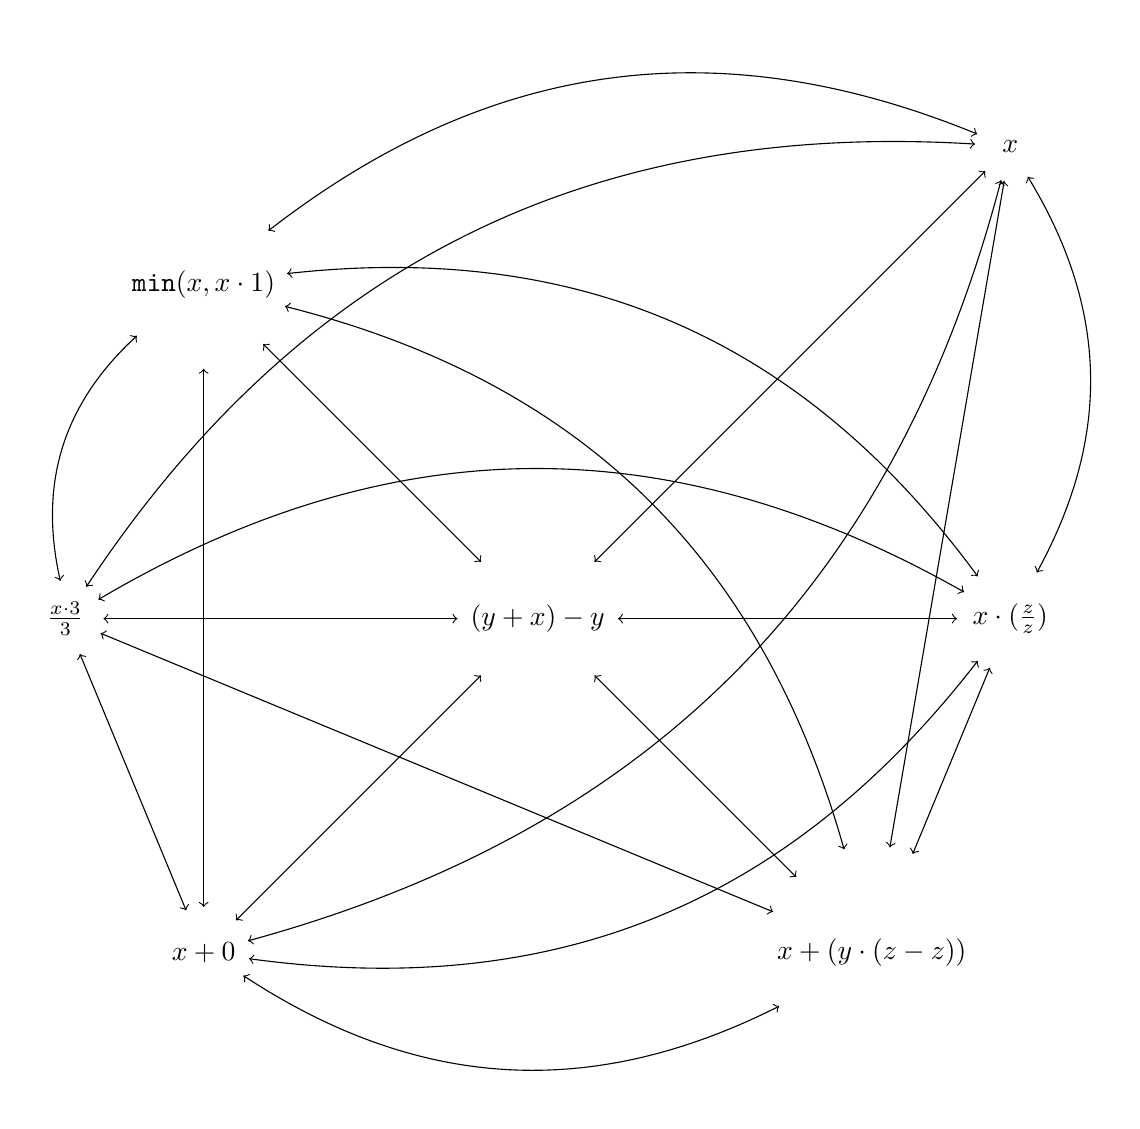
\begin{tikzpicture}[<->,auto,node distance=6cm]
\tikzstyle{every state}=[draw=none]
\node[state]    (A)     {$(y + x) - y$};
\node[state]    (B) [below left of=A]    {$x + 0$};
\node[state]    (C) [below right of=A]    {$x + (y \cdot (z - z))$};
\node[state]    (D) [right of=A]    {$x \cdot (\frac{z}{z})$};
\node[state]    (E) [above of=D]    {$x$};
\node[state]    (F) [above left of=A]    {$\hmin(x, x \cdot 1)$};
\node[state]    (G) [left of=A]    {$\frac{x \cdot 3}{3}$};

\path (A)   edge    node {} (B)
            edge    node {} (C)
            edge    node {} (D)
            edge    node {} (E)
            edge    node {} (F)
            edge    node {} (G)
     (B)    edge [bend right]   node {} (C)
            edge [bend right]   node {} (D)
            edge [bend right]   node {} (E)
            edge    node {} (F)
            edge    node {} (G)
    (C)     edge    node {} (D)
            edge    node {} (E)
            edge [bend right]   node {} (F)
            edge    node {} (G)
    (D)     edge [bend right]   node {} (E)
            edge [bend right]   node {} (F)
            edge [bend right]   node {} (G)
    (E)     edge [bend right]   node {} (F)
            edge [bend right]   node {} (G)
    (F)     edge [bend right]   node {} (G);

\end{tikzpicture}
\end{figure}


\subsection{Rationale for synthesis pipeline}

Here we lay out the rationale for our proposed synthesis pipeline. In particular, we will discuss three key assumptions: that a reduction order can be an effective heuristic for guiding term rewrites to a desired form; that a term rewriting system can be synthesized incrementally rule by rule; and that choosing candidate left-hand sides gathered from realistic inputs is an efficient means of finding rules that will have high impact on the performance of the term rewriting system.

When we specify a term rewriting system in this work, we say that it must have three properties:

\begin{itemize}
    \item it must be semantics-preserving
    \item it must terminate on all inputs
    \item it must rewrite terms into a form that has some desired property
\end{itemize}

The first two properties are required. As our language is undecidable, we can't create a TRS that is able to rewrite \emph{all} terms into the desired form. Our incremental synthesis pipeline is thus designed to grow the ruleset rule by rule, such that with each successful iteration of the synthesis algorithm, the ruleset is able to move more terms further toward the desired form.

In chapter~\ref{chapter:synthesis}, we showed that the Halide simplifier was semantics-preserving by verifying that for each rule $(l \rewrites r) \in R$, $l =_e r$, where the equality relation $=_e$ was checked via an SMT solver. We showed that the TRS was terminating by choosing an order $>$ over terms and showing that every rule in $R$ rewrote terms to be strictly less in that order. When we synthesized new rules to add to the simplifier ruleset, we did not explicitly define the third criterion, but allowed the termination order fitted to the existing ruleset to guide the synthesis pipeline. 

In this section, we will define more precisely the goal or intent behind a term rewriting system. We argue that an effective means of specifying this intent for the purpose of synthesis is to use a reduction order to capture the notion of rewriting a term to be closer to some goal state.

\begin{figure}
    \centering
\subfigure[$\termlang$]{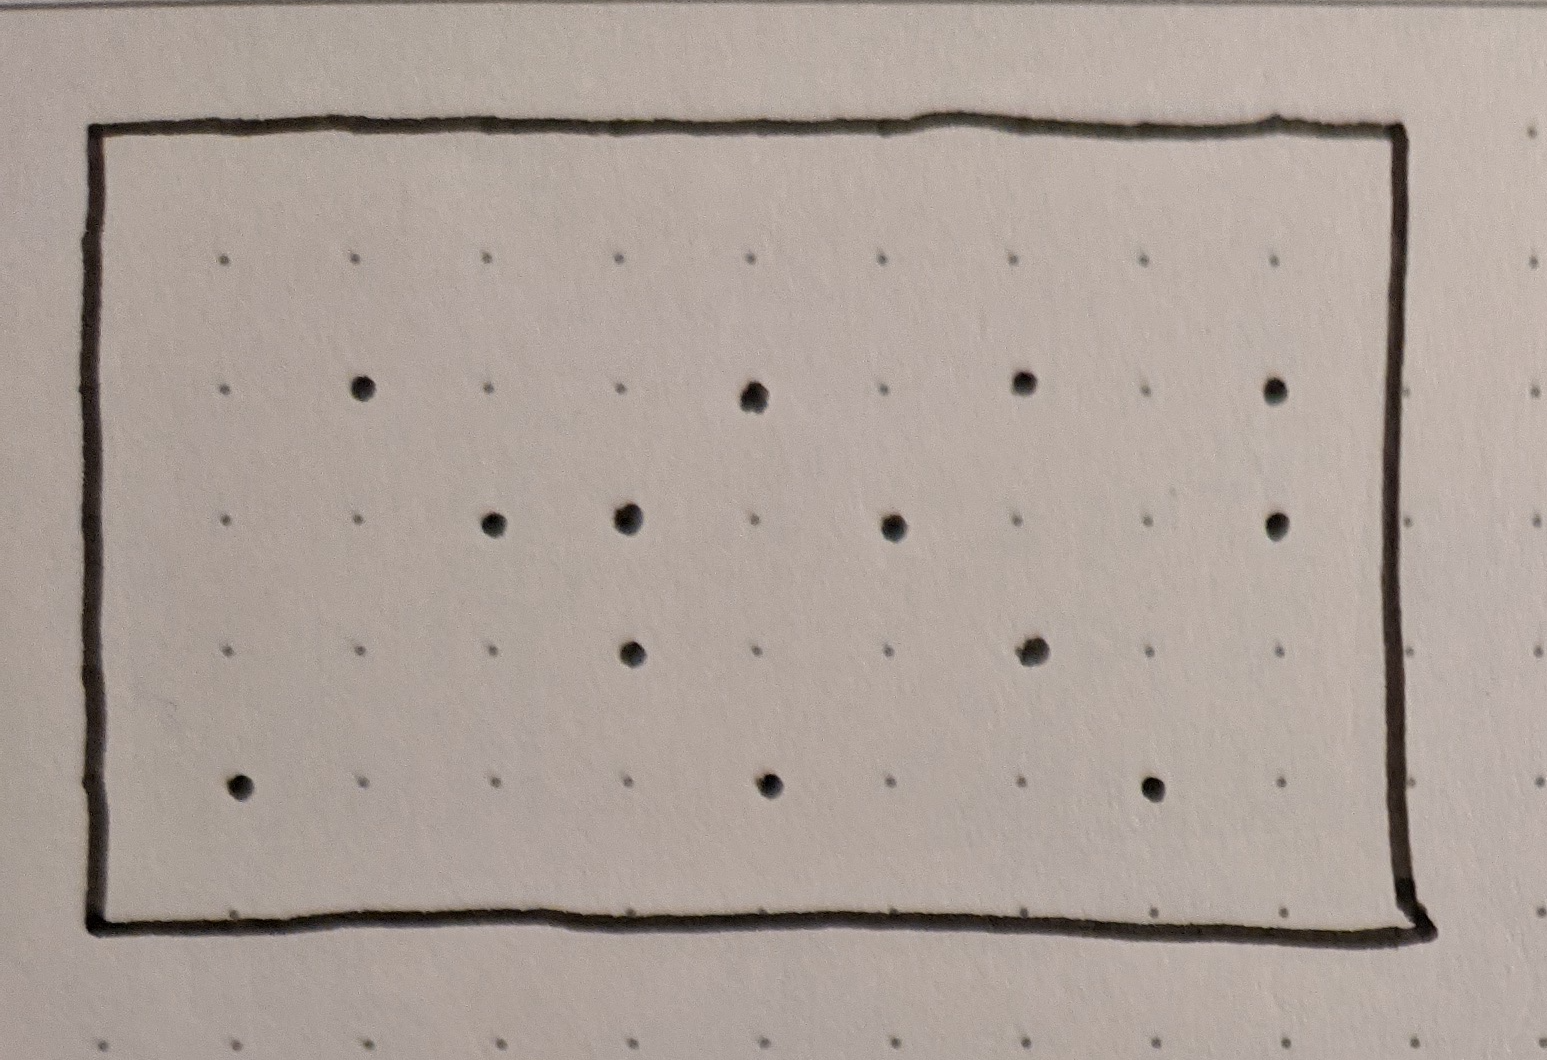
\includegraphics[width=0.3\textwidth]{figures/diagram1.png}}
    \hspace{1em}
    \subfigure[$\{s | s \in \termlang \wedge \phi(s)\}$ in red]{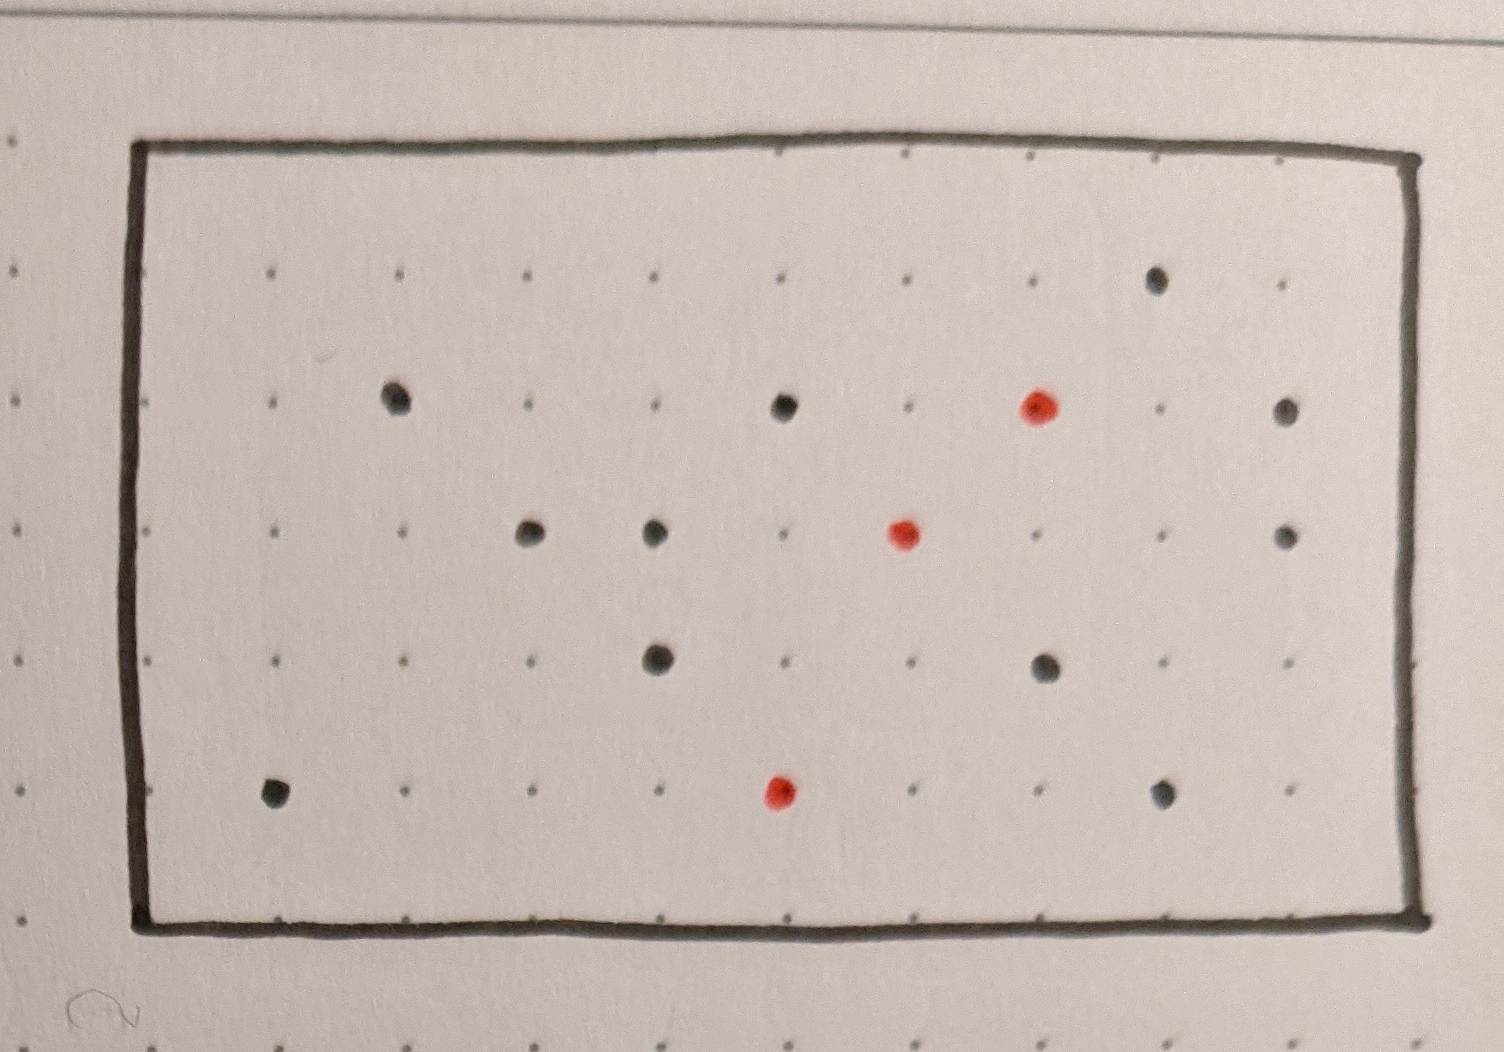
\includegraphics[width=0.3\textwidth]{figures/diagram2.png}}
    \hspace{1em}
    \subfigure[$\goallang$ in blue]{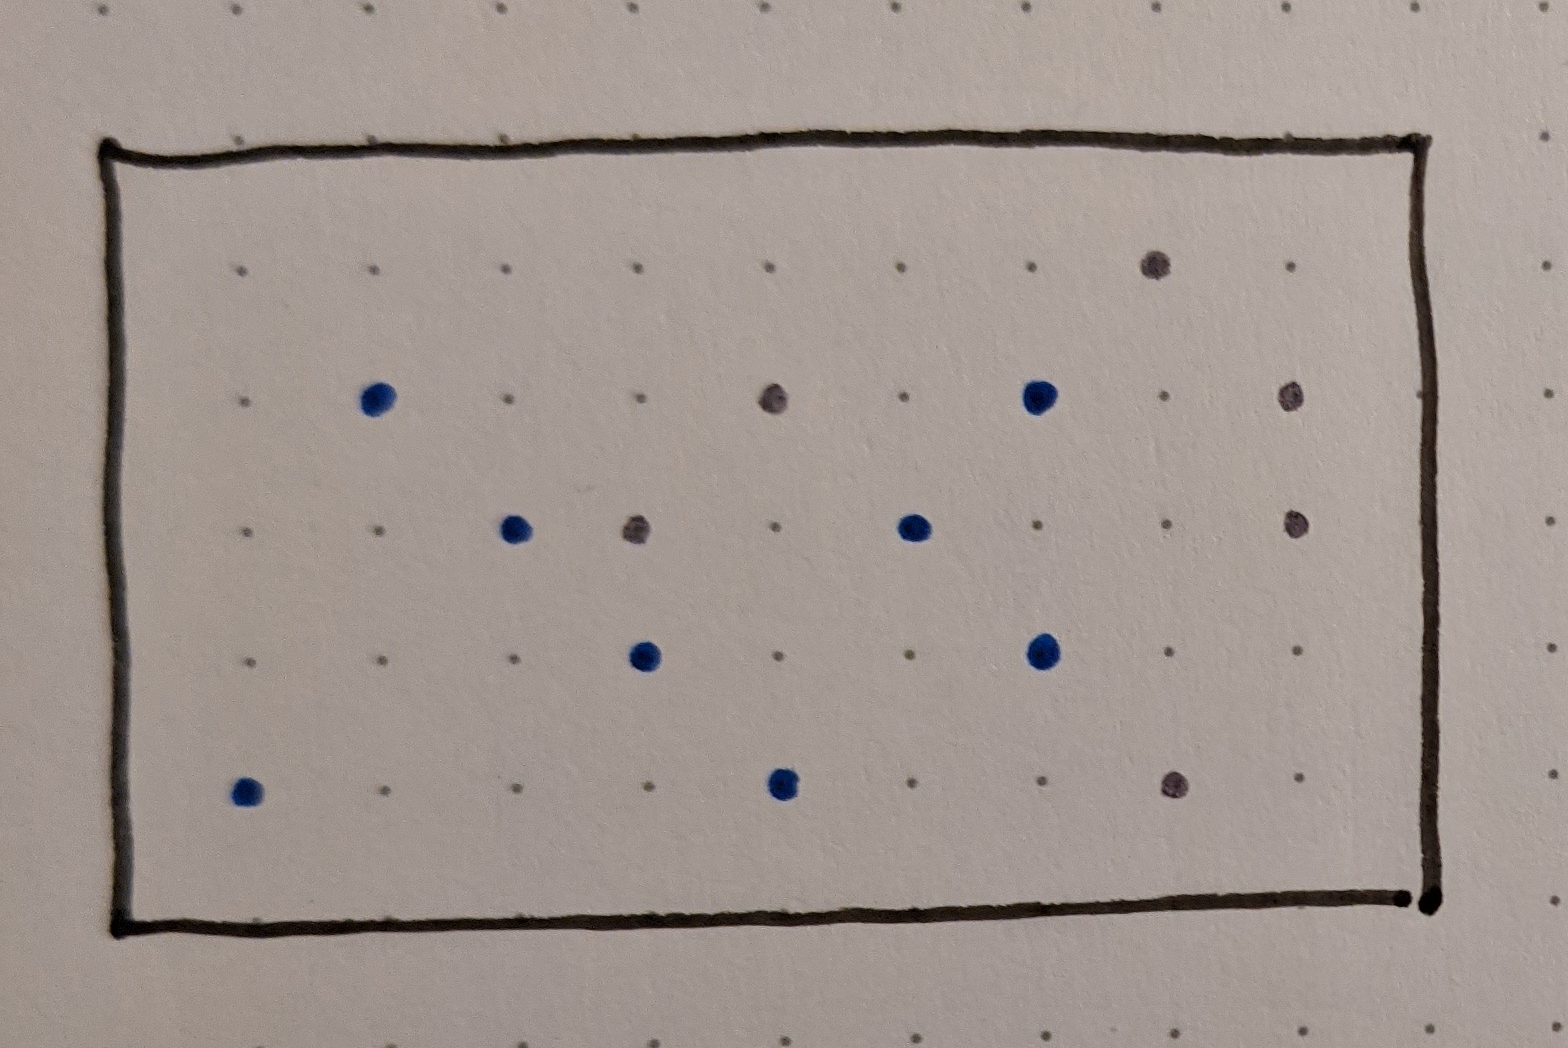
\includegraphics[width=0.3\textwidth]{figures/diagram3.png}} \\
    \subfigure[Undirected edges connect all $s, t$ st. $s =_e t$]{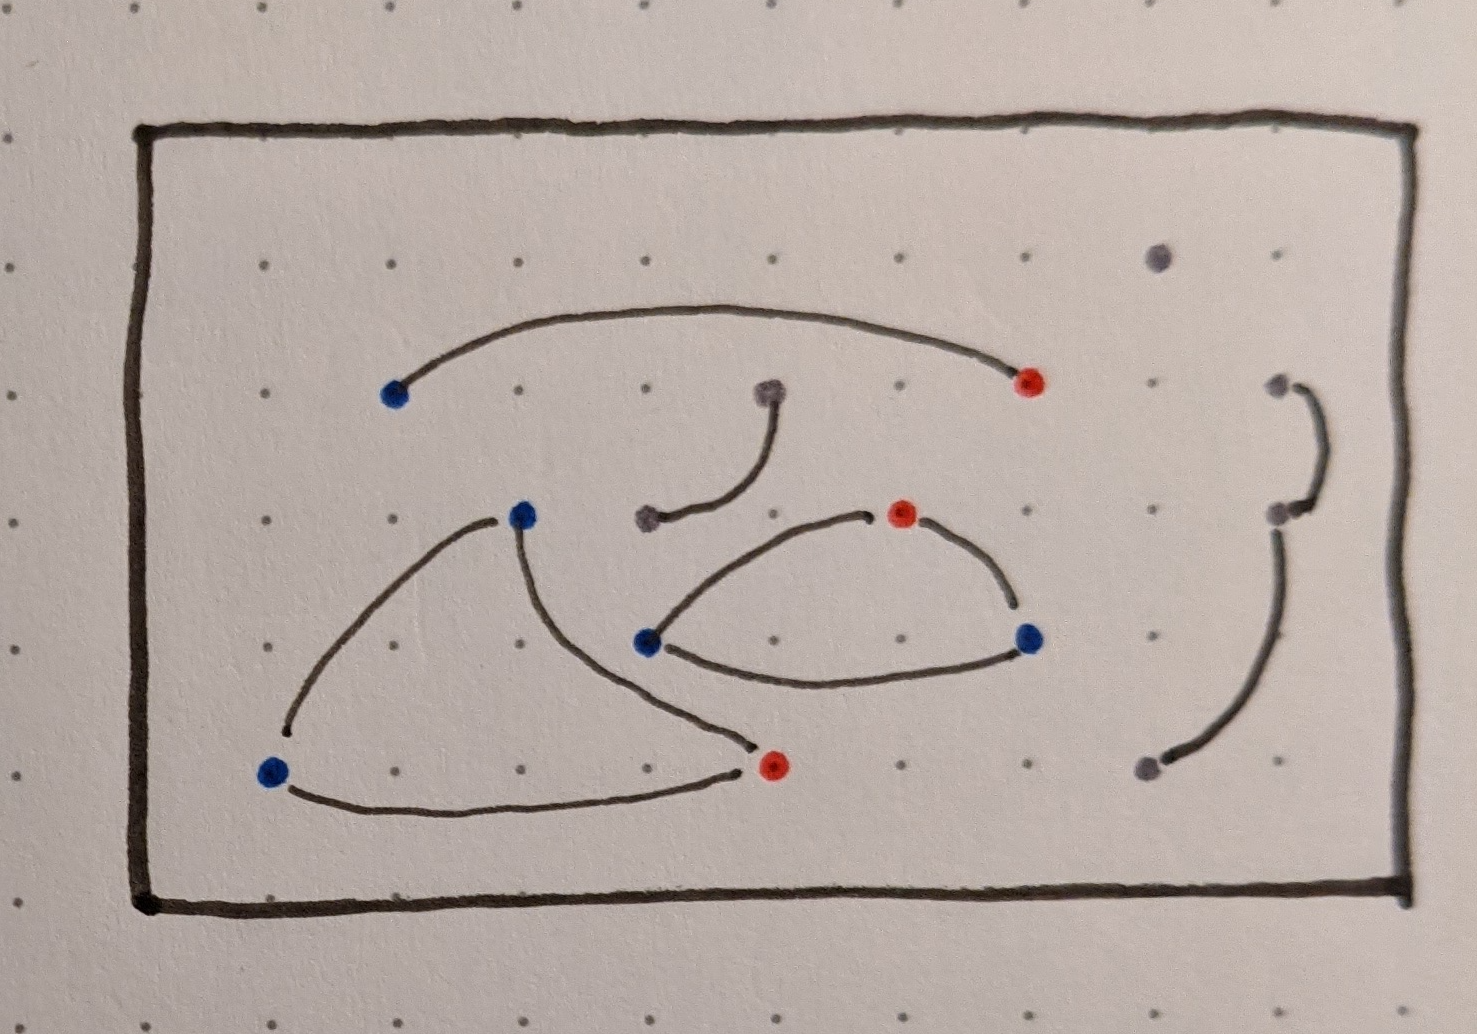
\includegraphics[width=0.3\textwidth]{figures/diagram4.png}}
    \hspace{1em}
    \subfigure[Directed edges connect all $s, t$ st. $s =_e t \wedge s > t$]{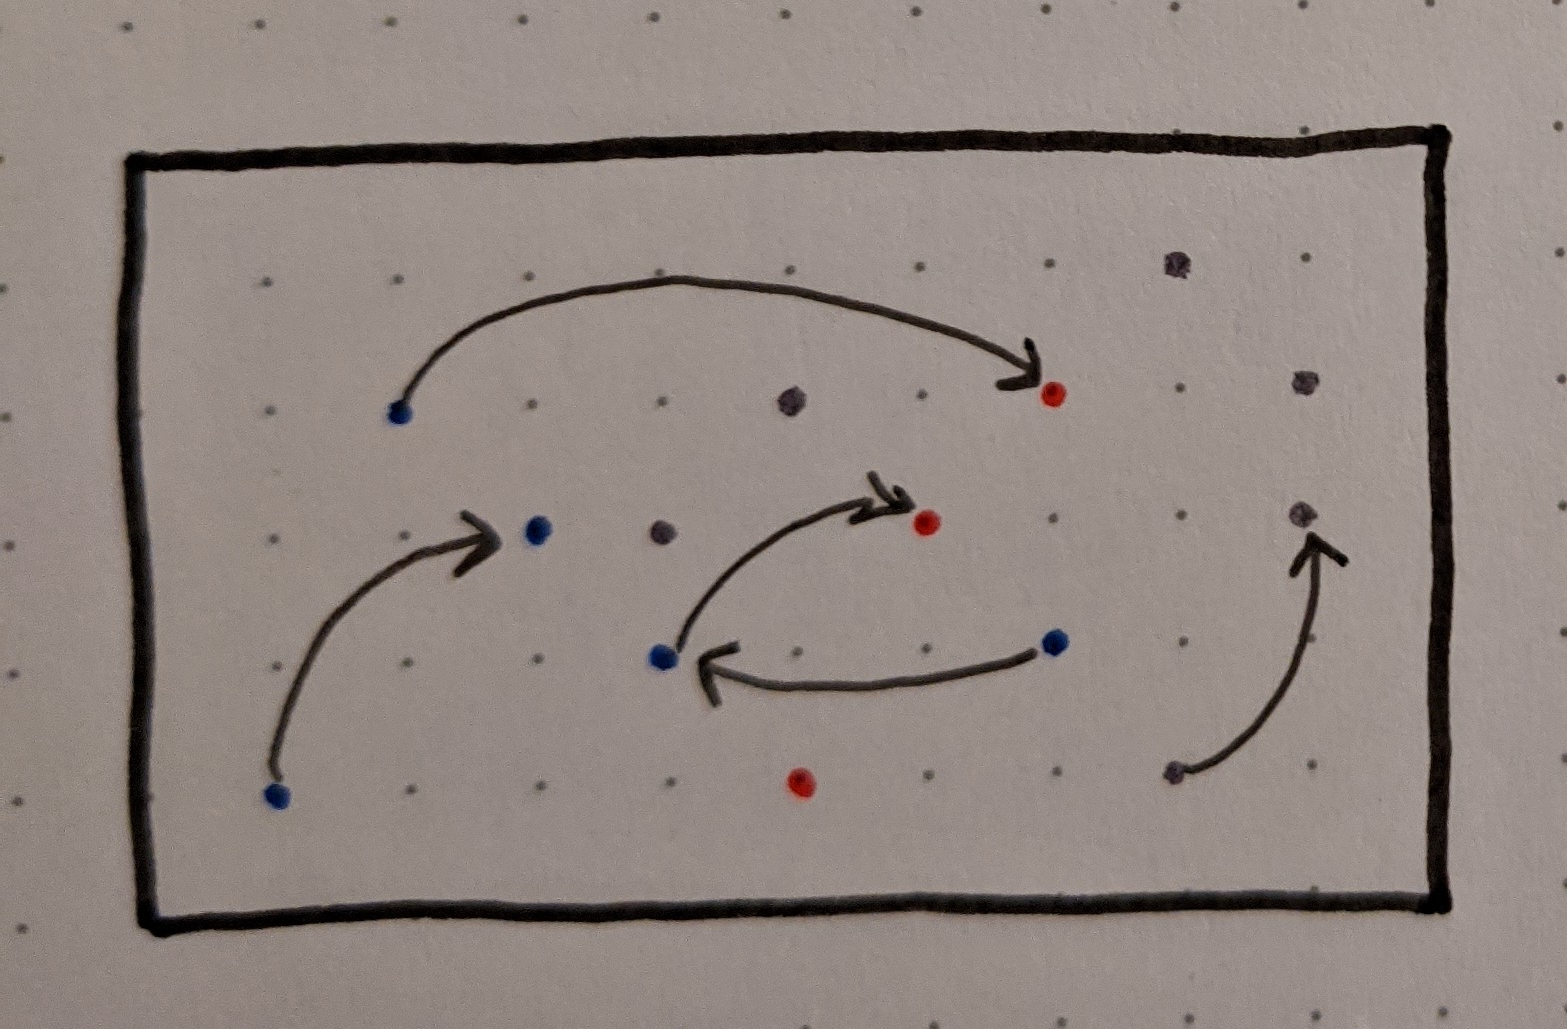
\includegraphics[width=0.3\textwidth]{figures/diagram5.png}}
    \caption{Each dot in (a) represents a term in $\termlang$. In (b), each term in the goal state is drawn in red. In (c), all terms which are equivalent to a term in the goal state ($\goallang$) are drawn in blue. The goal of the term rewriting system is to rewrite all blue dots in (c) to a red dot in (b). In (d), undirected edges connect all pairs of terms that are semantically equivalent. In (e), those edges have been oriented with a reduction order. Given the specification $\forall (l \rewrites r) \in R \st l =_e \wedge l > r$, we can find a TRS $R$ by picking a finite subset of all the directed edges in (e).}
    \label{fig:termuniverse}
\end{figure}

First, we define the goal property that describes the underlying intention of the term rewriting system. Assume some language of terms $\termlang$ and a semantic equivalence relation over those terms $=_e$ (as opposed to a syntactic equivalence relation, which we will write $=$). We write the goal property as a predicate function $\phi$ such that $\phi(s)$ is true if $s$ is in the goal state and false otherwise. 

We can thus write the domain of the term rewriting system as a language $\goallang \subseteq \termlang$, defined as

\[
\goallang = \{s | s \in \termlang \wedge (\exists t \in \termlang\;.\; s =_e t \wedge \phi(t))\}
\]

We want our term rewriting system to put every term in $\goallang$ into a form that satisfies our goal function $\phi$. When we specify how a term rewriting system rewrites terms into a goal state, we refer only to terms in $\goallang$; when the TRS rewrites a term that in is $\termlang$ but not in $\goallang$, it need only obey the semantics-preserving and termination properties.\footnote{We might prefer that the term rewriting system act on terms not in $\goallang$ as little as possible, but this is purely for performance reasons and can be set aside for now.}

To illustrate these definitions, we will develop formal specifications for two example term rewriting systems that represent different aspects of the Halide simplifier TRS. As discussed in section~\ref{sec:uses-of-trs}, the simplifier is used in many places in the Halide compiler under a number of difference circumstances, perhaps explaining the extremely complex reduction order we devised to fit its ruleset. Here, we will isolate two of the simplifier's important function: showing that a term must always evaluate to true, and showing that a term is strictly increasing or strictly decreasing.

 As in the rest of this work, we assume that $\termlang$ is the Halide expression grammar. First, we consider a prover TRS, which tries to determine if an expression is equivalent to the booleans values true or false, or if its truth value is unknown. We state that the prover has a domain language $\goallang_P$, which contains all terms in the Halide expression language that are equivalent ($=_e$) to $\htrue$ or $\hfalse$, and a goal state function $\phi_P$ that returns true if its input syntactically equivalent ($=$) to $\htrue$ or $\hfalse$ and false otherwise. This goal function encodes the purpose of the TRS, which is to transform all terms that are semantically equivalent to true or false to the boolean constants $\htrue$ or $\hfalse$. (Again, the goal function says nothing about terms in the Halide language, e.g. $x < y$, that are not provably true or provably false.)

\begin{align*}
    \phi_P(s) := s = \htrue \vee s = \hfalse
    \goallang_P = \{s | s \in \termlang \wedge (s =_e \htrue \vee s =_e \hfalse)\} \\
\end{align*}

The second example is a TRS that seeks to show that a given expression is monotonic. The goal function for this TRS is a bit more subtle. The Halide compiler's means of querying the monotonicity of an expression is sound but not complete: it walks the expression to see if it is in a syntactic form that can be recognized as monotonically increasing, monotonically decreasing, or constant. If it cannot recognize the expression as any of these three, it returns unknown. The job of the monotonic rewriter TRS is to put expressions into this syntactic form wherever possible. We say then that the domain language of the monotonic rewriter $\goallang_M$ is all terms $s$ in $\termlang$ where there exists some term $t$ such that $s =_e t$ and $t$ is in a syntactic form that can be recognized as monotonic or constant by the function $\texttt{is_monotonic}$ in the Halide codebase. The goal state function $\phi_M$ returns false when $\texttt{is_monotonic}$ returns unknown on an input term, and true otherwise. (Again, $\phi_M$ may return false for a term that is not in monotonic form because it is not in $\goallang_M$, i.e. no semantically equivalent monotonic form exists, but we can disregard this case for now.)

With these definitions in hand, we are now ready to formally specify the three properties we require of a term rewriting system (semantics-preserving, terminating, and rewrites terms into a desired form). We write $R(s)$ for the output of a term rewriting system $R$ on the input term $s$. Assume we use the means of assuring semantics preservation and termination as used above. Then, for an equivalence relation $=_e$ and a goal function $\phi$, we write that a specification for an ideal TRS $R$ thus:

\begin{align*}
\forall s \in \goallang \st \phi(R(s)) \wedge \\
\forall t \in \termlang \st t =_e R(t) \wedge R(t) \textrm{ terminates }
\end{align*}

Of course, since our theory is undecidable, the $\forall s \in \goallang \st \phi(R(s))$ portion of our specification is almost certainly unrealizable in the general case. Instead, we would like to encode a means of making progress towards this goal, rather than ruling out all TRSs that do not achieve it. We can think of this as a strategy for rewriting terms to be closer to the desired goal state. For example, imagine we started writing rules for the prover, and started with this pair:

\begin{align*}
    x = x \rewrites \htrue \\
    x + (y - y) \rewrites x
\end{align*}

We might note that the second rule is canceling like terms, and add many more rules that do the same. If we wanted to formally encode this strategy, we could do so using an order over terms, such that terms that satisfy the goal condition $\phi$ would be least elements in that order. In the case of the prover, the order could be to compare terms by their length; since the boolean constant $\htrue$ is of the shortest possible length in the Halide expression language, it is a least element of this order. Let us call such an order $\goalorder$ and add it as a condition to our specification:

\begin{align*}
\forall s \in \goallang \st \phi(R(s)) \wedge  s \geq_{\phi} R(s) \wedge \\
\forall t \in \termlang \st t =_e R(t) \wedge  R(t) \textrm{ terminates }
\end{align*}

As pictured in figure~\ref{fig:termuniverse}, the process of choosing rewrite rules for a ruleset is choosing edges from the graph (d) and orienting them. The goal order $\goalorder$ could be considered an order traversal from terms not in the goal state to terms that are. 

Now, assume we have been given some solution to our specification in the form of a term rewriting system $R$. How can we prove that it fulfills our criteria? In prior work, we proved that a term rewriting system was semantics-preserving ($\forall t \in \termlang \st t =_e R(t)$) and terminating ($\forall t \in \termlang \st R(t) \textrm{ terminates }$) by showing that those properties held over every rule in the ruleset. We can use a similar strategy here: if the goal order $\goalorder$ holds for every rule in $R$, then it must hold for all of $R$ as a whole.

\begin{assumption}
We can lower our requirement that the ruleset $R$ rewrite every term in $\goallang$ to the goal state to the requirement that every rule in $R$ rewrites terms to be closer to the goal state, as described by a goal order $\goalorder$.
\end{assumption}

% describe this more clearly: 
Requiring the goal order hold over every rule in $R$ will exclude some possible term rewriting systems for which the goal order would hold over the full system, just as requiring that the termination property hold over every rule in $R$ excludes some TRSs that are terminating. This is illustrated in figure~\ref{fig:termuniverse}; when we choose an order that turns the undirected edges in (d) to directed edges in (e), there are now some terms in $\goallang$ that are unable to reach a goal state. However, checking that this property holds over every rule can be done quickly and automatically. Just as with the termination guarantee, so long as every rule we add to a ruleset conforms to the goal order, we can add, delete, or permute the priority of rules without fear of losing our overall guarantee. This quick machine-checkable proof allows us to synthesize a TRS without human supervision.

In order for the goal order to hold over every term that may match and be rewritten by a rule, it must be a valid reduction order: well-founded, $\Sigma$-operation compatible, and closed under substitution (see~\citep{baader1999term}). Usefully, this means we do not need a separate termination order; since a goal order requires that each rewrite moves a term monotonically lower in the order, it also provides a termination guarantee.

We can now restate our term rewriting system specification like so:

\begin{align*}
    \forall s \in \goallang \st \phi(R(s)) \wedge \\
    \forall (l \rewrites r) \in R \st l =_e r \wedge l \goalorder r
\end{align*}

Since any term rewriting system we wish to synthesize will be semantics-preserving, the major decision we need to make in specifying a term rewriting system is to pick a goal order:

\begin{assumption}
We can effectively formalize the goal of a term rewriting system by choosing a \emph{goal order} over terms such that, for two terms $s$ and $t$ such that $s \goalorder t$ in this order, $t$ is assumed to be closer to the goal state.
\end{assumption}

Finding a goal order that encodes progress towards a goal state is a difficult task, and requires human intuition and ingenuity. Our work does not directly aid in this task, which is still up to the human author of the term rewriting system; however, our synthesizer machinery can aid in experimenting with and selecting goal orders.

\begin{table}[]
    \centering
    \begin{tabular}{|l|l|l|}
    \hline 
        TRS & Goal function $\phi$ & Goal order $>$ \\
        \hline 
        Prover &  $\phi(s)$ if $s$ is $\htrue$ or $\hfalse$ & $s > t$ if $t$ is shorter than $s$\\
        \hline
        Monotonic rewriter & $\phi(s) := \texttt{is_monotonic(s)}$ & $s > t$ if $s$ has more $\%$ ops \\
                 & & $s > t$ if $s$ has more constants \\
        \hline
    \end{tabular}
    \caption{Two term rewriting systems, goal functions that encode their intent, and goal orders that represent moving towards those goals}
    \label{tab:trsspecs}
\end{table}

As discussed above, the prover could adopt a strategy of making expressions shorter, with the aim of eventually being able to reduce them to the constants $\htrue$ or $\hfalse$. For the monotonic rewriter, one expression in the goal state is $x \cdot c_0$ where $c_0$ is a positive constant; the monotonicity checker recognizes this form as monotonically increasing. So, one possible strategy could be to move constants to the right side of an equation wherever possible. We may also want to employ sub-strategies: if the prover TRS contains the rule $x = x \rewrites \htrue$, we might choose a strategy of putting expressions into a kind of canonical form wherever possible, so we can rewrite an expression $e_1 = e_2$ into $e' = e'$ and then apply the identity rewrite rule. The simplifier reduction order, which was composed of several orders lexicographically, could be said to employ a series of sub-strategies in this way. See table~\ref{tab:trsspecs} for the prover and monotonic rewriter goal functions and some goal orders that approximate them.
 % check with Andrew about monotonic rewriter example

If we accept the assumption that a reduction order can encode the strategy of rewriting a term to be closer to our goal, we now have a specification that should hold for every individual rule we synthesize:

\[ \forall (l \rewrites r) \in R \st l =_e r \wedge l \goalorder r
\]

The set of possible rules made up of terms in the Halide expression language that conform to that spec is still infinitely large. The other part of our spec required that $\forall s \in \goallang \st \phi(R(s))$, but this is unrealizable. Instead we relax to a specification that could actually be checked; for example, we could fix a set $S$ of terms and write that our term rewriting system should:

\begin{align*}
    \forall s \in S \st \phi(R(s)) \wedge \\
    \forall (l \rewrites r) \in R \st l =_e r \wedge l \goalorder r
\end{align*}

Now we have a realizable synthesis procedure: we can synthesize rules $(l \rewrites r)$ such that $l =_e r \wedge l \goalorder r$, add them to $R$, and terminate when $\forall s \in S \st \phi(R(s))$ holds, as described in algorithm~\ref{algo:synthesis}. In practical cases, we may want to use other termination conditions, such as requiring that some fraction of $S$ can be solved. In our prior work, we did not check that the outputs of the synthesis-augmented simplifier brought previously unsolved terms to the goal state at all, but relied on a fairly complex goal order to produce a strengthened ruleset that was demonstrably more effective on our benchmarks.

Finally, we need a strategy for choosing which rule to add to growing ruleset at each step. As the space of potential rules is so large, even if term sizes are bounded, simply sampling at random may not be effective. Our synthesis pipeline defines a strategy for growing a ruleset so that it is able to rewrite more and more of $\goallang$, in a way that is of practical benefit to the compiler. In prior work, we gathered a corpus of expressions seen by the compiler in realistic circumstances and mined them for general patterns to form candidate LHS terms. We then attempted to synthesize RHSs for each candidate LHS term to form rules. We assert that this is an effective method of creating a ruleset is effective under realistic workloads.

\begin{assumption}
An effective heuristic for choosing candidate left-hand side terms for new rules is to gather expressions seen by the compiler under realistic circumstances and mine them for general patterns.
\end{assumption}

Note that when we gathered input expressions in prior work, we did not check to see if those expressions were in the TRS domain $\goallang$. Any means of checking membership in $\goallang$ is necessarily incomplete, so any ruleset learned from a checked input list would inherit the incompleteness of the checker. Also, note that we will want to rewrite subterms of expressions that are not themselves in $\goallang$: in the prover TRS, although all input expressions are boolean-valued, we will want to rewrite subterms of all possible types. For example, given the ruleset $R = \{x = x \rewrites \htrue, x + x \rewrites x \cdot 2\}$, we need the second rule that rewrites a numeric-valued expression so that we can rewrite $x + x = x \cdot 2$ to $\htrue$.

Given these three assumptions, we propose the synthesis pipeline in algorithm~\ref{algo:synthesis}. 

\subsection{The Halide variable solver}

The Halide simplifier was a fairly mature system, in production for over a year and consists of almost a thousand rules. The Halide variable solver, by contrast, is a much smaller system, currently implemented as a series of if statements rather than a formal term rewriting system, and consisting of the equivalent of less than a hundred rules. The simplifier's use cases were quite varied and complex, and the existing ruleset required a complex composite reduction order to cover their full purpose. The variable solver is much smaller and more focused and can be captured by much simpler reduction orders. With the variable solver, therefore, we have the opportunity to experiment with various reduction orders to find the one that fulfills the system's purpose best, and to synthesize a TRS entirely from scratch, rather than augment an existing system.

% synthesis pipeline: Rosette, encoding reduction order as metasketches, metasketch search order, etc
% discussion of different granularities of reduction order
% evaluation of various synth'd TRSs

\section{The variable solver reduction orders}

Here we refer to \emph{target-matching variables} as variables that can be unified with the target variable or subterms that contain the target variable. Variables that cannot be unified with the target variable or subterms that contain the target variable are called \emph{non-target-matching variables}. All variables that occur in the variable solver ruleset are either target-matching or non-target-matching. Allowing variables that can match either target variable-containing subterms or non-target variable containing subterms complicates reduction order definitions. \jln{is it true that any rule containing variables that can match anything can be replaced by multiple rules that only contain target-matching or non-target-matching variables?}

We represent target-matching variables as $x^t, y^t$, etc., and non-target-matching variables as $x^n, y^n$, and so on.

\subsection{Reduce occurrences of target-matching variables}

\[ s_1 >_t s_2 \iff \forall x^t \in \mathcal{V}(s_1) |s_1|_{x^t} \geq |s_2|_{x^t}
\]

The proof that this order is a valid reduction order is straightforward. The order is clearly well-formed, since $|s|_{t_i}$ has a minimum value of 0. The order is compatible with $\Sigma$-operations; for any

\[ s_1 >_t s_2 \implies f(t_1,...t_{i-1},s_1,t_{i+1},...,t_n) >_t f(t_1,...t_{i-1},s_2,t_{i+1},...,t_n)
\]

\begin{align*}
\sum_{x^t \in \mathcal{V}} \sum_{0}^{i - 1} |t_k|_{x^t_k} + |s_1|_{x^t_k} + \sum_{i + 1}^{n} |t_k|_{x^t_k} >
\sum_{x^t \in \mathcal{V}} \sum_{0}^{i - 1} |t_k|_{x^t_k} + |s_2|_{x^t_k} + \sum_{i + 1}^{n} |t_k|_{x^t_k}
\end{align*}

Since $|s|_{x^t}$ is always non-negative, the implication clearly holds.

Finally, the order is closed under substitutions. A substitution $\sigma$ could increase the number of target-matching variables in $s_2$ by replacing some $x^t$ with a subterm containing multiple target-matching variables, but since all target-matching variables in $s_2$ must occur an equal or greater number of times in $s_1$, the order must be preserved. Any substitution for a non-target-matching variable will have no effect on the number of target-matching variables in $s_1$ or $s_2$ by definition. 

Note that this order does not require that the number of non-target-matching variable occurrences in $s_1$ be equal or greater to the number of occurrences in $s_2$; it is perfectly fine to increase the size of the rewritten expression so long as the count of target-matching variables goes down. For example, the rule $t_0 <= (t_0 + n_1) \rewrites n_1 >= 0$ introduces a new constant on its RHS, but obeys the order as it reduces the number of occurrences of $t_0$.

\subsection{Move occurrences of target-matching variables to the left}

The intuition behind the order is simple, but we will have to take care in our definition to make sure it is a valid reduction order. We define this order by transforming terms into strings and then comparing the strings lexicographically.

To transform a term into a string (we write this function as $\texttt{varstr}(s)$), we first take the sequence of all occurrences of variables and constants in the term, in the order in which they occur. We truncate the sequence by removing everything after the last occurrence of a target-matching variable. We then replace all target-matching variables with 'a' and all non-target-matching variables or constants with 'b', and compare the resulting string with that of another term in lexicographic order (such that a $<$ b).

\begin{tabular}{l|l|l|l}
\centering
$n_0 + t_0 > t_0 + n_0$ & $(n_0 t_0) > (t_0 n_0)$ & $(n_0 t_0) > (t_0)$ & ab $>$ a \\
\end{tabular}

This order is clearly compatible with $\Sigma$-operations; if $\texttt{varstr}(s_1) > \texttt{varstr}(s_2)$, then the order will still hold if identical prefixes and suffixes are added to both terms. 

\begin{align*}
s_1 > s_2 \implies & f(t_1,s_1,t_n) > f(t_1,s_2,t_n) \\
\texttt{varstr}(s_1) > \texttt{varstr}(s_2) \implies & \texttt{varstr}(t_1) + \texttt{varstr}(s_1) + \texttt{varstr}(t_n) > \\
&\texttt{varstr}(t_1) + \texttt{varstr}(s_2) + \texttt{varstr}(t_n)
\end{align*}

However, we need to add an additional condition to make the order closed under substitution. Consider a rule

\[ (n_0 + n_1) + (t_0 + n_2) \rewrites (n_2 + t_0) + (n_0 + n_1)
\]

The rule appears to move the target-matching variable to the left and thus seems to be in conformance with the order. However, given the substitution $\sigma = \{ n_0 \mapsto y^n, n_1 \mapsto z^n, t_0 \mapsto x^t, n_2 \mapsto ((u^n + v^n) + w^n)\}$, we obtain the transformation
\[ (y^n + z^n) + (x^t + ((u^n + v^n) + w^n)) \rewrites (((u^n + v^n) + w^n) + x^t) + (y^n + z^n)
\]

which actually shifts the target-matching variable to the right. The problem occurs because the non target-matching variables have been reordered from the LHS term to the RHS. A similar issue arises if we reorder the target-matching variables:

\begin{align*}
(t_0 + n_0) + t_1 \rewrites & (t_1 + t_0) + n_0 \\
\sigma = \{ t_0 \mapsto x^t, n_0 \mapsto y^n, t_1 \mapsto ((z^n + w^n) + x^t)\} \\
(x^t + y^n) + ((z^n + w^n) + x^t) \rewrites & (((z^n + w^n) + x^t) + x^t) + y^n
\end{align*}

To disallow this ordering, we add the condition that a rewrite rule that follows this order cannot permute the sequence of target-matching variables or the sequence of non-target-matching variables; it can only change how the two sequences are interleaved. More precisely, if we take the sequence of target-matching variable instances from $s_1$ and $s_2$, we should be able to fix a mapping from each variable instance in $s_2$ to an instance of that same variable in $s_1$ such that, after deleting all variable instances in $s_1$ that are not mapped, the two sequences are identical. We must be able to do the same with the non variable-matching variables in both terms, after omitting all non target-matching variables that occur after the final instance of a target-matching variable in their respective terms. With these condition, there is no substitution that can introduce a non target-matching variable in the $s_2$ term without introducing at the same or earlier position in $s_1$, maintaining the order.

\subsection{Move occurrences of target-matching variables up}

Similar to the previous order, this order is an intuitive step in isolating the target variable to the left of a top-level binary operator. To define this order formally, we first define a function \texttt{bfs_hash} that takes a term and a variable, and returns a hash whose keys are the depths of the AST representation of that term and whose values are the number of instances of that variable that occur at those depths. We say that $\texttt{bfs_hash}(s_1, x) < \texttt{bfs_hash}(s_2, x)$ if $\texttt{bfs_hash}(s_1, x)[0] < \texttt{bfs_hash}(s_2, x)[0]$, or if $\texttt{bfs_hash}(s_1, x)[0] = bfs_hash(s_2, x)[0] \wedge \texttt{bfs_hash}(s_1, x)[1] < \texttt{bfs_hash}(s_2, x)[1]$, and so on.

We then say that $s_1 >_\uparrow s_2$ if, for every target-matching variable $x_t$ that occurs in $s_1$, there are an equal or greater number of occurrences of that variable in $s_1$ than in $s_2$, and $\texttt{bfs_hash}(s_1, x) \leq bfs_hash(s_2, x)$, and if there exists at least one target-matching variable whose \texttt{bfs_hash} value is strictly greater in $s_2$ than in $s_1$.

\begin{align*}
s_1 >_\uparrow s_2 \iff & \forall x^t \in \mathcal{V}(s_1) \st (|s_1|_{x^t} \geq |s_2|_{x^t} \wedge \\
                        & \texttt{bfs_hash}(s_1, x_t) \leq \texttt{bfs_hash}(s_2, x_t)) \\
                        & \wedge \exists x^t \in \mathcal{V}(s_2) \st \texttt{bfs_hash}(s_1, x_t) < \texttt{bfs_hash}(s_2, x_t))
\end{align*}

For example, consider the rule

\[ (t_0 - n_0) < n_1 \rewrites t_0 < (n_0 + n_1)
\]

Both the LHS and RHS have the same number of target-matching variables. \texttt{bfs_hash}($(t_0 - n_0) < n_1, t_0$) = $\{0: 0, 1: 0, 2:1\}$, while \texttt{bfs_hash}($t_0 < (n_0 + n_1), t_0$) = $\{0: 0, 1: 1, 2:0\}$. As \texttt{bfs_hash}($(t_0 - n_0) < n_1, t_0)[0] = \texttt{bfs_hash}(t_0 < (n_0 + n_1), t_0)[0]$ and \texttt{bfs_hash}($(t_0 - n_0) < n_1, t_0)[1] < \texttt{bfs_hash}(t_0 < (n_0 + n_1, t_0))[1]$, the order holds over this rule.

This order has a least element with regard to a fixed number of target-matching variables: one in which all target-matching variables occur in the highest level of the AST. As the number of target-matching variables in any RHS must be less than or equal to the number of target-matching variables in the LHS, it is not possible to construct an infinitely descending chain in this order, so the order is well-founded.

The order is $\Sigma$-compatible; for each target-matching variable, \texttt{bfs_hash}($f(t_1,\dots,t_{i-1},s_1,t_{i-1},\dots,t_1$) is the sum of the \texttt{bfs_hash} of its subterms (with the depths incremented by one). As \texttt{bfs_hash}($f(t_1,\dots,t_{i-1},s_2,t_{i-1},\dots,t_1$) is the sum of precisely the same subterms but with $\texttt{bfs_hash}(s_1)$ replaced by $\texttt{bfs_hash}(s_2)$, the requirement holds.

The order is also closed under substitutions. As all variables are necessarily terminals in a given AST, substituting a subterm for a given variable cannot ``push down'' any part of the term that is not directly part of the substitution. Any substitution for a non-target-matching variable will have no effect on the \texttt{bfs_hash} output. For every instance of a target-matching variable in a RHS term, we can fix a corresponding instance of that same variable in the LHS term at an equal or lower depth. Any change to the \texttt{bfs_hash} counts therefore cannot possibly result in a violation of the order.

\subsection{Put rewritten expression into fully solved form}

The orders described above describe a strategy for manipulating terms towards the goal state of putting them in fully solved form. Is it possible to encode the goal state directly as an order? Recall that we defined `solved form' as:

\begin{enumerate}
  \item $|t|_{x^t} = 0$ (the term $t$ does not contain the target variable $x^t$).
  \item $t = x^t$ (the term $t$ is precisely the target variable $x^t$).
  \item $t = x^t \odot t'$, where $\odot$ is any binary function in $\Sigma$, and $|t'|_{x^t} = 0$. Terms in this form are only considered 'solved' if no term $u$ in either of the above two forms exist such that $t =_e u$.
\end{enumerate}

Reduction orders must be checkable syntactically, so we relax the requirement that the second form is only considered solved if no equivalent term in the first form exists and so on. Then, we can formalize these forms into orders such that terms that are solved are ordered less than terms that are not solved.

\begin{enumerate}
    \item $s_1 >_{f1} s_2 \iff \exists x^t \in \mathcal{V}(s_1) \wedge \neg \exists x^t \in \mathcal{V}(s_2)$
    \item $s_1 >_{f2} s_2 \iff \exists x^t \in \mathcal{V}(s_1) \wedge s_1 \neq x^t \wedge s_2 = x^t$
    \item $s_1 >_{f3} s_2 \iff s_1$ cannot match $f(t_0, n_0)$ for any $f \in \Sigma$, and $s_1$ can match $f(t_0, n_0)$ for some $f \in \Sigma$
\end{enumerate}

Are these valid reduction orders? All three are well-founded, in that they partition the set of all expressions into two equivalence classes (expressions in solved form and expressions not in solved form) and orders all members of the first class as less than the second. However, none of the three are $\Sigma$-compatible; if an expression in solved form is added as a subterm in a larger expression, the new expression is necessarily not in solved form. The second and third orders are also not closed under substitution; in the second and third type of solved form expression, if the single $x_t$ variable is substituted for a longer term containing a target-matching variable, the resulting expression will not be in solved form. (The first order is closed under substitution, since we can substitute any non-target-matching variable with any term not containing a target-matching variable and remain in solved form.)

This demonstrates that any specification for a ruleset will represent a strategy for rewriting expressions towards a goal state, and not necessarily a means of putting expressions into a goal state in all circumstances. Consider the following rule, whose RHS is in solved form

\[ (t_0 + n_1) == n_0 \rewrites t_0 == (n_0 - n_1)
\]

which can be used to rewrite the following three expressions

\begin{align*}
x_t + y_n = z_n \rewrites x_t = z_n - y_n \\
(z_n < w_n) \&\& x_t + y_n = z_n \rewrites (z_n < w_n) \&\& x_t = z_n - y_n \\
(x_t * 3) + y_n = z_n \rewrites (x_t * 3) = z_n - y_n 
\end{align*}

In the first instance, the rewritten expression is in solved form, but the second and third instances are not.

Although the `solved form' orders are not valid reduction orders, it seems clear that rulesets following these orders must terminate, and in fact this is true. For any rule that obeys one of the above orders, its RHS will be the least element of one of the reduction orders we outlined above. Thus the rule will conform to a reduction order, and any such ruleset is guaranteed to terminate.

\begin{tabular}{l|l}
$s_1 >_{f1} s_2$ & $s_1 >_{t} s_2$ \\
$s_1 >_{f2} s_2$ & $s_1 >_{\leftarrow} s_2$ \\
$s_1 >_{f3} s_2$ & $s_1 >_{\uparrow} s_2$
\end{tabular}

We could thus think of rules that obeyed the `solved form' orders as rules that take the largest possible step in the direction of the goal state. If we limited our ruleset to such rules, would the result be more powerful than a ruleset that allowed all rules that obey the reduction orders above? We will investigate this in our evaluation.

\section{The synthesis algorithm}

Our synthesis algorithm takes as inputs 

\begin{itemize}
\item A goal function $\phi$, which returns true when applied to a term in the goal state and false otherwise. 
\item A semantic equivalence relation $=_e$ over terms. A concrete implementation of this relation is required to be sound, but it will almost certainly be incomplete (unless working in a decidable theory).
\item A reduction order $>$, which encodes a desired strategy of moving terms in the direction of the goal state.
\item A set of training expressions $E$, which will be used to choose candidate left-hand sides for new rules. These expressions should be likely inputs to the TRS when it is used for its desired task.
\item A set of test expressions $S$, which will be used to determine if the synthesized TRS is powerful enough, or if we should continue learning new rules.
\end{itemize}

An idealized version of the algorithm is presented in Algorithm~\ref{algo:synthesis}. We initialize with an empty ruleset $R$. While there is some expression in our test set $S$ that $R$ cannot rewrite to satisfy the goal function $\phi$, we will attempt to learn a new rule. We choose an expression from our training set $E$, and from that expression choose a pattern that could match with it to serve as a candidate left-hand side. We query the synthesizer for a right-hand side that is semantically equivalent to the LHS and is ordered less than the LHS in our reduction order. If we cannot find such a RHS, we choose another candidate LHS and continue. When we do find a RHS that satisfies our specification, we have learned a new rule. We add this new rule to the end of the ruleset $R$. We then use the updated ruleset to rewrite every training expression in $E$, discarding any expressions that can satisfy $\phi$ after being rewritten (since the newly updated TRS is capable of rewriting those expressions to the goal state, we do not need to learn any more rules from these expressions). The remaining expressions in the updated set $E$ have been rewritten as far in the direction of the goal state as the new ruleset is capable of. If the test set condition is not yet met, we want to learn rules that will bring these expressions even further toward the goal state, so we choose a candidate LHS on our next iteration from this newly normalized set.

\begin{algorithm}[H]
\SetAlgoLined
\KwIn{goal function $\phi$, semantic equivalence relation $=_e$, reduction order $>$, set of training expressions $E$, set of test expressions $S$}
\KwResult{a term rewriting system $R$}
\While{$\exists s \in S \st \neg \phi(R(s))$}{
    choose $e \in E$, $l \in \texttt{lhs\_patterns(e)}$\;
        query synthesizer for $r$ such that $l =_e r \wedge l > r$\;
    \If{$r$ is found}{
        $R \gets  R \bigcup \;\{(l \rewrites r)\}$\;
        $E \gets \{ R(e) | e \in E \wedge \neg \phi(R(e))\}$\;
    }
}
\caption{Idealized procedure for synthesizing a term rewriting system}
\label{algo:synthesis}
\end{algorithm}

(implementation of synthesis pipeline outlined here, full section TK)

Implemented in Rosette. How Rosette works. Chosen for quick development of pipeline and to take advantage of symbolic evaluation/some built-in simplification. Wrote an interpreter for the Halide expression language in Rosette. In order to handle the disparity between Halide/C++ semantics and Racket semantics, had to add some lightweight typing to prevent integer-valued expressions being used as boolean. Also div/mod issues (depending on if we fix this or just skip it).

Built a term rewriting system algorithm with target-variable aware matching. Cite TRaAT ML code. Also reduction order checkers.

In the variable solver synthesis pipeline, we begin with a set of likely inputs to the desired TRS. 

Grow ruleset rule by rule. Every time we learn a rule, we add it to the end of the ruleset, normalize the input by the new rule, and continue.

Choose an initial input expression. We iterate over subterms in the order that the rewriting algorithm would attempt to match them, bottom-up depth first search order. Basically we attempt to rewrite an expression the way a term rewriting system would, but appealing to a solver to find any solution it can rather than precalculated rules.

From the chosen subterm, find all patterns that could match it. On the rationale that more general rules are more useful, we sort the resulting patterns by size and try the smallest first.

Now we have a candidate left-hand side expression. We attempt to form a rule by synthesizing a matching right-hand side. Using Rosette's synthesis construct, we write a query stating for all variables, the candidate LHS should be semantically equivalent to the synthesized RHS. This satisfies the requirement that a rewrite rule should be semantics-preserving.

We also need to fulfill our specification expressed as a reduction order. Rather than express this requirement as an assertion that the synthesized solution must satisfy, we instead use the reduction order to constrain the search space available to the solver by encoding the order as a sketch. Talk about sketches and metasketches.

\subsection{The fully solved order as sketches}

The fully solved order is a composition of three orders.

\subsubsection{No target variables sketch}
The only constraint on a sketch of this kind is that the synthesized solution does not contain any of the target variables. Write as register program, searching from instruction count 1 to instruction count k where k is the number of operators in the LHS expression.

\subsubsection{Target variable alone sketch}
Note that while the no target variable order is ahead of this order in the fully solved order composition, if a solution in this form exists, then there is no solution in the form of a term that does not contain any target variables, and vice versa. 

For each unique target variable in the LHS expression, we attempt to verify that the LHS expression is semantically equivalent to that target variable. If we are successful, this forms a new rule.

\subsubsection{Target variable op expression sketch}
For each unique target variable, we ask the solver to choose some binary operator from the Halide expression language whose left operand is that target variable and whose right operand is an expression that does not contain any target variables. We synthesize this right operand using a register-style sketch as above, searching from instruction count 1 to instruction count k.

\subsection{The gradual order as sketches}

\subsubsection{Fewer target variables order sketch}

\subsubsection{Move target variables left order sketch}

\subsubsection{Move target variables up order sketch}

\section{Evaluation of synthesized TRSs}
\label{sec:varsolvereval}

To evaluate our synthesis process, we attempted to synthesize term rewriting systems that could make meaningful progress on a realistic set of benchmarks. We gathered a set of expressions by instrumenting calls to the existing Halide variable solver and running a suite of applications with randomly generated schedules. As our current synthesis pipeline does not support synthesis of rules guarded by predicates, there was no need to consider constant values, so we replaced all constants in the gathered expressions with fresh variable. After removing all duplicate expressions modulo alpha renaming, we had a set of 4218 expressions to serve as benchmarks. Note that not all of these benchmarks can be put into solved form, and since we lack a decision procedure for this undecidable problem, we do not know how many of the benchmarks can be solved.

We chose 33 of those expressions as a training set. We chose these expressions randomly, excluding expressions that were so large as to cause performance issues during synthesis. Recall that the Halide rewriting algorithm attempts to rewrite each subterm of an expression, and that each subterm can be matched by many potential LHS patterns. Thus, the set of 33 expressions yielded about 500 candidate LHS expressions (depending on how successful the learned TRS is at rewriting expressions---if a rule is learned that can transform an input expression, the newly rewritten expression may yield more candidate patterns).

We ran two synthesis experiments, taking as a specification the goal form order and the gradual order respectively. The goal form order task synthesized 21 rules, while the gradual order task synthesized 32. All of the rules in the goal form TRS were also present in the gradual TRS. Both the goal form and gradual TRS are able to solve 11 of the 33 training set expressions. 

Of the 4218 benchmarks (including the 33 training set expressions), the goal form TRS was able to put 949 of them into solved form, while the gradual TRS was able to solve 966 of them; in other words, the goal form TRS performed fairly well and the gradual TRS performed slightly better. There were 18 expressions that the gradual TRS was able to solve that the goal form TRS was not. In all 18 cases, both TRSs applied the same sequence of rewrites up to a certain point, when the goal form TRS was unable to continue. The gradual TRS was able to further rewrite the expression with a rule that was not present in the goal form TRS, and from there was able to continuing rewriting the expression into a solved form.

For example, consider this input expression~\footnote{The expression has been simplified by replacing subterms that have no bearing on the final result with fresh variables. For example, $\frac{y + c_0}{c_1} \cdot c_1$ has been replaced by $y$.}

\[ \hmax{(((y + ((x + z) - w)) + c_1), (u + ((z + x) - w)))} + (w - (x + z))
\]

Both the goal form and gradual TRS rewrite it to

\[ (x + \hmax{((((z - w) + y) + c_1), ((z - w) + u))}) + (w - (x + z))
\]

at which point no rules in the goal form TRS can be applied. However, the gradual TRS can apply the rule

\[ t_0 + (n_1 - t_2) \rewrites t_0 - (t_2 - n_1)
\]

to produce the expression

\[ ((x + max((((z - w) + y) + c_1), ((z - w) + u))) - ((x + z) - w))
\]

The gradual TRS can then apply further rewrites to cancel the target variable and arrive at an expression in solved form:

\[ \hmax{((((z - w) + y) + c_1), ((z - w) + u))} - (z - w)
\]

Interestingly, in 15 of the 18 expressions that the gradual TRS was able to solve when the goal form TRS was not, the rule that unlocked the expression for the gradual TRS was actually one that obeyed the goal form order. Recall that when we synthesize rules from an input expression, we attempt to rewrite it just as we would with a concrete TRS, but rather than rewriting with existing rewrite rules we ask the solver if we can find a new rule that would allow us to make progress. On the input expression

\[ (x \cdot c_0) + ((y + z) - (((\frac{(select(c_1 < x, c_2, c_1) + z) + y}{c_3} + (x \cdot c_3)) \cdot c_3)))
\]

Both tasks were able to normalize to the following form using rules they already knew

\[ (x \cdot c_0) + ((y + z) - (((\frac{(select((x > c_1), c_2, c_1) + (z + y))}{c_3}) + (x \cdot c_3)) \cdot c_3))
\]

From there, the goal form order task was not able to learn any new rules. However, the gradual order task was able to apply one more rule to the expression, which moves a target variable to the left but does not put the term into fully solved form.

\[ (n_0 + n_1) - t_2 \rewrites n_0 - (t_2 - n_1)
\]

The gradual order task was then able to learn two new rules from the resulting expression, including one in goal form order

\[ (t_0 - n_1) - n_2 \rewrites t_0 - (n_2  + n_1)
\]

Although this rule obeys the goal form order, the goal form order task never encountered the input expression that would have matched its LHS, and so it never synthesized the rule.

It is perhaps not surprising that a TRS is able to successfully rewrite more expressions than a TRS that is its strict subset. More surprising is the fact that the goal form TRS was able to solve one expression that the gradual TRS could not. On the benchmark expression~\footnote{Similarly simplified.}

\[ (((y + z) - x) \cdot c_1 - w) + (x \cdot c_1 + u)
\]

the goal form TRS immediately applies a rule that cancels out the target variable.

\begin{align*} 
((((n_0 - t_1) \cdot n_2) - n_3) + ((t_1 \cdot n_2) + n_4)) & \rewrites ((n_4 - n_3) + (n_0 \cdot n_2)) \\
(((y + z) - x) \cdot c_1 - w) + (x \cdot c_1 + u) & \rewrites ((u - w) + ((y + z) \cdot c_1))
\end{align*}

However the gradual TRS first applies a rule not in the goal form TRS

\begin{align*}
(n_0 + n_1) - t_2 & \rewrites n_0 - (t_2 - n_1) \\
(((y + z) - x) \cdot c_1 - w) + (x \cdot c_1 + u) & \rewrites ((y - (x - z)) \cdot c_1) - w) + (x \cdot c_1 + u)
\end{align*}

Although the gradual TRS contains the rule the goal form TRS used to reach solved form, this additional rewrite means that the rule no longer applies, and the gradual TRS gets stuck. We will discuss this type of problem more fully in section~\ref{sec:completion}, but for now we will observe that adding new rules is not an unalloyed good.

We also compared the performance of our synthesized TRSs against several other TRSs we constructed. First, we translated the `rules' in the C++ version of the variable solver currently in the Halide compiler into formal rewrite rules. We removed any rules that were guarded by predicates, as our synthesis process does not currently support rule predicates. We then filtered that ruleset by the two reduction orders for comparison. (In fact, when running the unfiltered ruleset on the benchmarks, it failed to terminate, from which we can conclude that there is no reduction order that can be made to fit the full original ruleset. The Halide compiler version terminates now because it does not recurse on every rewrite but in certain cases simply returns.)

When the `original' ruleset was filtered by the gradual order, it consisted of 75 rules, more than twice the size of the synthesized gradual TRS. However it performed surprisingly poorly, solving only 106 benchmarks. However, it was able to solve 21 benchmarks that the synthesized gradual TRS was not.

When verifying the rewrite rules in the simplifier, we had to prove some of them were sound using the proof assistant Coq. The Coq standard library contains a large set of integer axioms, and we wondered how powerful those axioms might be as a TRS. We chose the relevant integer axiom libraries, scraped them for axioms, and transformed those axioms into rewrite rules by considering each assignment of target-matching and non-target-matching status to the variables in each equality and retaining any equality that could be oriented using one of our two reduction orders. The resulting TRS using the gradual reduction order was quite large, 480 rules, but was only able to solve 792 benchmarks, 174 fewer than the synthesized ruleset. It was able to solve 107 benchmarks that the synthesized TRS could not, however. Filtering the Coq TRS by the goal form order resulted in a much smaller ruleset (148 rules) with very similar solving performance (787 solved benchmarks). 

In an earlier synthesis experiment, we tried using smaller inputs for our training set. Our reasoning was that smaller inputs would quickly yield small, highly general rules, which would allow a TRS to be bootstrapped more quickly. We sorted the 4218 benchmarks by size and chose the smallest 400 expressions as a training set, synthesizing using the gradual reduction order as a specification. The resulting 38-rule TRS was able to solve only 492 of the full benchmark set; it was able to solve 66 expressions that the first synthesized gradual ruleset was not. Its training set contained patterns that the previous training set did not; for example, both TRSs learned the rule $n_0 \leq t_1 \rewrites t_1 \geq n_0$, but only the TRS trained on the shorter expressions learned the rule $n_0 \geq t_1 \rewrites t_1 \leq n_0$. For comparison's sake, we filtered the small-inputs synthesized TRS by the goal form order, resulting in a TRS of 29 rules. This was the only case in which the goal form order version of a TRS performed markedly worse than its gradual counterpart; it solved only 251 benchmarks and only 44 that the synthesized gradual TRS could not solve.

Finally, observing that all of these TRSs solved at least one expression that the synthesized gradual TRS could not, we took the union of \emph{all} of the TRSs by simply concatenating all the rulesets into one. The resulting union TRS performed the best of all, solving 1124 benchmarks including 179 that the synthesized gradual TRS could not. Filtering the union TRS by the goal form order, however, resulted in even better performance with 1180 expressions solved. Much like the one expression that the synthesized goal form TRS could solve but the synthesized gradual TRS could not, clearly some of the rules in the union gradual TRS are preventing helpful rewrites from occurring. Again, we will further discuss this issue in~\ref{sec:completion}.\jln{TODO: union ruleset sizes are approximate because the same rule appears in multiple TRSs in the union; get the accurate counts.}

\begin{tabular}{l|r|r|r}
Name & $|R|$ & Solved exprs & Solved exprs not solved by Gradual \\
\hline
Synthesized Gradual & 32 & 966 & 0 \\
Synthesized Goal form & 21 & 949 & 1 \\
Original (gradual) & 75 & 106 & 21 \\
Original (goal form) & 53 & 105 & 20 \\ 
Coq axiom & 480 & 792 & 107 \\
Coq axiom (goal form) & 148 & 787 & 103 \\
Small inputs & 38 & 492 & 66 \\
Small inputs (goal form) & 29 & 251 & 44 \\
Union & ~625 & 1124 & 179 \\
Union (goal form) & ~253 & 1180 & 218
\end{tabular}


\section{Related work}
\label{sec:related}

Perhaps the closest related work is the Alive project~\citep{lopes2015alive,menendez2017aliveinfer}.
The fundamental difference between Alive and this
work is that Alive works within the decidable theory of bitvectors, while
(because of Halide semantics) we must use the undecidable theory of integers;
this constraint is the major reason for many of our design choices. In addition:
Alive verifies optimizations (and Alive-Infer synthesizes preconditions), while
we synthesize rewrites and predicates, as well as verify them; Alive must contend
with more types of undefined behavior, which the Halide expression
language need not consider; and Alive uses a simple reduction order in
which all optimizations reduce program size, while our termination proof is more
complex. We originally tried synthesizing rule predicates with the approach used
by Alive-Infer but were not successful: using Z3 to generate positive and
negative examples did not scale for us, requiring seconds to minutes per query
due to the underlying theory of integers.  Moreover, queries with
division/modulo over the integers often did not work at all, simply returning
``unknown.''

Most recently, leveraging a TRS along with synthesized rules has been applied
to optimizing fully-homomorphic encryption (FHE) circuits~\citep{lee2020fhe}.  This
system synthesizes equivalent circuits with lower cost from small example circuits,
then applies the equivalences in a divide-and-conquer manner; the rewrites do
not contain preconditions. In further contrast to our work, the domain of FHE yields a
simple cost function (the depth of nested multiplications in the circuit), and
the underlying theory of boolean circuits is decidable.

Herbie~\citep{panchekha2015automatically}, a tool for improving the accuracy of floating point arithmetic, uses an egraph term rewriting system made up of a small library of axioms to find repairs once a fault has been localized. Herbie assures termination by bounding the number of rewrites their system may apply, and achieves good performance by pruning the expression search space and applying rewrites only to particular expression nodes. 

Besides the closely-related projects described above, program synthesis has been applied to term rewriting systems in several domains. Swapper~\citep{singh2016swapper} synthesizes a set of rewrite rules to transform SMT formulas into forms that can be more easily solved by theory solvers, similar to the use of the Halide TRS as a simplifier, using the SKETCH tool. \citep{butler2017synthesizing} learns human-interpretable strategies (essentially rewrite rules) for puzzle games such as Sudoku or Nonograms and \citep{butler2018framework} finds tactics for solving K-12 algebra problems, both using a CEGIS loop similar to our synthesis process. None of these address termination, although Swapper likely screens out non-terminating rulesets through its autotuning step. The Butler works both focus on synthesizing small, highly general rulesets that are similar to human rewriting strategies, unlike the Halide TRS which tolerates very large rulesets.  The \textbf{$\lambda^2$} tool~\citep{feser2015lambda} for example-guided synthesis performs inductive synthesis from examples, using a combination of inductive and deductive reasoning combined with enumerative search.  While our rewrite rules do not have the benefit of examples, it may be possible to apply this technique to obtain more sophisticated predicate synthesis for our rewrites.

Superoptimization, a process of finding a shorter or more desirable program that is semantically equivalent to a larger one, is similar to our work synthesizing right-hand side terms for candidate LHSs. STOKE~\citep{schkufza2013stochastic} uses Monte Carlo Markov Chain sampling to explore the space of x86 assembly programs, while \citep{phothilimthana2016scaling} describes a cooperative superoptimizer that searches for better programs using multiple techniques in a way that allows them to learn from each other.  Souper~\citep{sasnauskas2017souper} is a recent synthesis-based superoptimizer for LLVM, which was used in evaluating the effectiveness of Alive-Infer's{} precondition synthesis.

PSyCO~\citep{lopes2014weakest} synthesizes preconditions that guarantee a compiler optimization is semantics-preserving, using a counterexample-driven algorithm similar to our rule CEGIS loop (although not like our predicate synthesis algorithm). PSyCO finds the weakest precondition from a finite language of constraints, while the space of our predicate search is theoretically inifinite but in practice bounded by our iteration limit. PSyCO must reason about side effects by tracking read and write behavior in optimization templates, while our expression language is side effect--free. More recently, Proviso~\citep{astorga2019learning} finds preconditions for C\# programs using an active learning framework composed of a machine learning algorithm for decision trees as a black-box learner and a test generator that acts as a teacher providing counterexamples. Like this work, the logic of preconditions they synthesize is in an undecidable domain.

Other software that can solve equations in the manner of the Halide variable solver include SymPy~\citep{10.7717/peerj-cs.103}, MATLAB~\citep{higham2016matlab}, and GNU Octave~\citep{eaton1997gnu}. We plan to benchmark various synthesized versions of the Halide variable solver against these tools. 
\chapter{Conclusion and Future Work}
\label{chapter:conclusion}



\section{Future Work}

\subsection{Replacing the Halide variable solver}
\label{sec:varsolverreplacement}

In our evaluation (section~\ref{sec:varsolvereval}), we showed that we were able to synthesize effective term rewriting systems to address the variable solver's task. However, our ultimate, practical aim is to synthesize a term rewriting system that can replace the existing variable solver in the Halide compiler altogether. There are three main issues that need to be addressed before we can achieve that goal.

\subsubsection{Support for rule predicates}
In our previous evaluation, we did not attempt to synthesize predicates that must be fulfilled for a rule to be applied, as we did in the simplifier work. For that reason, we replaced all constant values in our benchmarks with fresh variables. However, calls to the variable solver frequently involve constants that are known at compiler time, as seen in the TrimNoOps example use case in section~\ref{sec:trimnoops}. Rules that can exploit information about those constants to apply further rewrites could be crucial in solving expressions that our synthesized TRSs cannot solve now.

Our process for synthesizing rule predicates for the simplifier was fairly involved and computationally expensive. However, we believe we could take a much simpler approach for the variable solver. For the simplifier, we first synthesized a RHS for a LHS expression that contained constants, then replaced those constants with fresh variables. If the equivalence between LHS and RHS no longer held, we attempted to synthesize a predicate that implied that equivalence. For the variable solver, rather than attempt to synthesize arbitrary predicates, we believe we could get similar performance with a small set of fixed predicates, such as $c > 0$, $c < 0$, $c \neq 0$, and conjunctions of the above. For each candidate LHS, we might choose one of those fixed predicates and a (symbolic) constant in the LHS to apply the predicate to, and ask the solver to find a RHS that is equivalent to the LHS assuming that predicate is true. This would multiply the number of queries to the solvers up to the size of the predicate set, but for a relatively small set this is still highly tractable.

\subsubsection{Support for division and modulo}
Integer division and modulo operations are difficult for SMT solvers such as Z3 to reason about, as discussed in section~\ref{sec:rhssynthesis}. In earlier experiments, candidate LHSs that contained division and modulo operations almost always resulted in solver queries that timed out, and very very few RHS expressions that contained those operations were ever synthesized. For that reason, in the variable solver experiments in section~\ref{sec:varsolvereval}, we skipped all candidate LHSs that contained division or modulo and removed those operations from the language grammar from which RHSs were synthesized. This saved large amounts of processing time and made virtually no different to the synthesized results. However, the variable solver is frequently invoked on expressions that contain those operations, so it will be important for the variable solver TRS to be able to handle them. We plan to investigate more performant ways to reason about these operations, such as approximating integers with bitwidth encodings.

\subsubsection{Conclusive benchmarks}
Our evaluation showed that a relatively small, randomly sampled training set is sufficient to learn a ruleset that is capable of solving a sizable fraction of a much larger test set. However, in order to propose a TRS that can serve as a substitute for the existing variable solver, we need a benchmark set that acts as a good proxy for realistic workloads the Halide compiler will encounter in the wild. We propose to work with Halide developers to gather such a benchmark set. We also did not demonstrate that a TRS-based variable solver with greater solving power would produce beneficial downstream effects in compiled pipelines, as we did for the simplifier; such a demonstration would be a useful argument for replacing the existing code with a synthesized TRS.

No matter how confident we are in our choice of benchmarks, it is difficult to draw a bright line and declare a synthesized TRS to be good enough---it is always possible to continue learning new rules, as our problem remains undecidable in the general case. 

\subsection{Completion}
\label{sec:completion}

\subsection{Completeness of the Halide TRS}
\label{sec:completion}

We know by observation that the Halide simplifier TRS cannot prove certain equalities 
that are in fact true, or reduce certain expressions that can be further simplified. 
Our goal is to learn new rules that would strengthen the TRS and allow it to make
further progress on these ``stuck'' expressions. This goal seems similar to that of 
\emph{completion}, which constructs a decision procedure through syntatic rewrites
for a set of identities. We do not use completion directly, although
our synthesis algorithm could be considered analogous to completion in some ways.

In the standard Knuth-Bendix completion algorithm~\citep{knuth1983simple}, we take a
finite set of identities $E$ and a reduction order $>$ on terms as inputs; if successful, the
algorithm will return a finite, convergent set of rules $R$ that is equivalent to 
$E$. The algorithm may also fail, or fail to terminate. At each step the algorithm
maintains a set of identities and a set of rules, both of which can be updated; the 
algorithm may transform an identity into a new rule, find a new identity as a 
consequence of the ruleset, or use the present ruleset to refine either an identity 
or a rule. The algorithm runs until the ruleset has converged; specific implementations
may use some conditions under which to terminate with a failure.

No finite set of identities exists for the theory of integers. We could
fix a set of identities to use in a completion procedure, but choosing these axioms
is a non-trivial task. One issue is that the theory contains axioms such as commutativity;
an identity such as $x + y \equiv y + x$ cannot be oriented by any possible reduction 
order, so our completion algorithm cannot make use of this fact. Another is that any
sufficiently powerful set of identities would almost certainly result in a non-terminating
completion procedure.  In addition, even if we use a subset of the Halide TRS for our
identities (thus yielding a confluent Halide TRS), our experience shows that many
failures in the compiler's use of the TRS are due to missing semantic facts that are not
derivable from the current Halide ruleset.

%%% SAK: I integrated this into a sentence above.  Not sure we need this much text.
%% \modified{One approach might be to transform the existing Halide TRS into a set of undirected
%% identities $E_R$ and use it together with a reduction order as inputs to a completion procedure. 
%% If successful, this would yield a confluent TRS, for which any sequence of rewrites to 
%% an expression would ultimately yield the same result. (It is not immediately clear how 
%% to handle rule predicates in this case, however.) While this is certainly desirable, 
%% our experience is that many proof failures in the current Halide TRS is not due to a 
%% lack of confluence, but because of knowledge of the Halide expression langauge semantics 
%% not encompassed by the identities in $E_R$.}

%Instead, our synthesis algorithm seeks to learn rules which cannot (necessarily) be 
  %deduced from the existing ruleset.
In the absence of a finite set of identities, we
treat an SMT solver as a decision procedure to determine if a suggested identity 
holds in our theory (of course, the solver itself is also incomplete; we only make use of the 
soundness of the solver and cannot derive any information in the case where the solver cannot
show that an identity holds). If the identity holds and can be oriented using our reduction order, 
it is added as a rule. It is possible that the newly-synthesized rule may be a consequence 
of the existing ruleset and thus could have been found by running completion, 
but we know that many synthesized rules contain information that is previously 
unknown to the TRS.

If we consider our solver as standing in for an infinite set of identities that make up
our theory, we clearly could synthesize an infinite number of rules. Here we make use
of the fact that expressions encountered by the compiler have some bias 
and are not sampled randomly from the entire expression space. In a preliminary 
experiment, we tried generating LHSs at random within a certain expression size and 
synthesizing RHSs to serve as new rules. We were able to find an extremely large number of 
``missing'' rules not represented in the current TRS, but the new ruleset had 
no measurable performance impact on benchmarks. Thus, we only synthesize rules if their LHS could be 
applied to at least one expression observed by the compiler under realistic usecases. %Even 
%without a formal definition of the bias on encountered expressions, we are able to 
%target synthesis to produce new rules that have some impact on compiler output.


%\sak{Should we say something about how this applies to things other than Halide?}

As we observed in the variable solver evaluation, adding a new rule is not guaranteed to strictly increase the number of benchmarks a TRS can solve. Particularly, we saw a case in which the synthesized goal form TRS was able to solve a particular expression when the synthesized gradual TRS was not; the application of a rule that only existed in the gradual TRS blocked the use of a rule that could have fully solved the expression. This occurred because the gradual TRS was not \emph{confluent}. In a confluent ruleset $R$, for any expression $s$, if some sequence of rule applications from $R$ can transform $s$ to $t$, and some other sequence of rule applications can transform $s$ to $t'$, then both $t$ and $t'$ must be eventually rewritten by $R$ to the same form $u$. In other words, $R$ will always normalize its inputs to the same form no matter what order rewrites are applied in. 

If a ruleset $R$ is finite and terminating, then a decision procedure exists to determine whether or not $R$ is confluent. Thus, we are able to detect if adding a new rule to a ruleset we are synthesizing would change it from confluent to non-confluent, giving rise to potential issues like the failing benchmark above. If we can detect these issues, can we address them at the time the rule is synthesized?

One strategy is suggested by \emph{completion} algorithms. A completion algorithm takes a set of (undirected) equalities and a reduction order and returns a terminating, confluent term rewriting system that has the same expressive power as the set of equalities. As a term rewriting system is also a set of (directed) equalities, these algorithms can also transform a non-confluent TRS into a confluent one. However, success is not guaranteed; the algorithm may succeed, fail, or fail to terminate. Thus naively running a completion algorithm on a synthesized ruleset will not necessarily prevent these issues and may also be computationally expensive. However, we plan to investigate how a modified completion algorithm could be used to prevent some instances of non-confluence without paying a large penalty in either performance or in ruleset size.

\subsection{Other Future Work}

As discussed earlier, choosing a gradual order that describes a strategy or gradient towards a desired goal form is not a trivial task and requires human intuition. Not only must the order describe a gradient over terms towards the goal, but it also must be a valid reduction order; if it is not, then the resulting term rewriting system (as well as the synthesis pipeline that produces it) is not guaranteed to terminate or indeed to actually make progress towards the goal. Proving an order is a valid reduction order is sometimes tricky, and appealing orders are often found not to be valid reduction orders after closer inspection. Reduction orders over terms often follow a set of patterns, such as orders that reduce the size of expressions or reduce the number of particular operations or variables. It would be a useful contribution to produce a handbook of these reduction order families, as well as strategies for efficiently encoding them into sketches for synthesis.

Finally, we intend to explore other applications of this work to other problems, other types of rewriting, and other domains. For example, synthesizing rewrite rules for a very different rewrite algorithm such as within an e-graph might require a very different strategy. Likewise synthesizing a term rewriting system for a decidable theory, such as bitwidths of finite width or linear integer arithmetic might also look very different.

\section{Conclusion}
We claim in this work that formal methods and program synthesis can be used to assist compiler authors in creating and maintaining these term rewriting systems. In prior work, we have shown how these techniques can aid in the maintenance of existing term rewriting systems by providing proofs of correctness and termination, and by synthesizing rewrite rules that strengthen a system's reasoning power. In proposed work, we plan to show how our techniques can greatly improve smaller or immature term rewriting systems or even create them from scratch. We have demonstrated the former claim in a case study on the Halide simplifier term rewriting system, and have presented a plan to investigate the latter claim on the variable solver, a much less mature term rewriting system in the Halide compiler.

The Halide TRS is used both to prove expressions true or false and to
simplify expressions to more easily optimizable forms, but these two use cases
are not always aligned. One could imagine two separate rewriters with
different rulesets and reduction orders. One interesting direction for future
work might be to use the synthesizer to create these two rulesets, which would
otherwise be a very human-effort intensive task.

Although we do not currently synthesize rules that contain vector operators,
they are not incompatible with our approach. Since our reduction of Halide
expressions to SMT2 formulas models vector expressions as integers, we would need
to add a typechecking step to ensure correctness in the synthesis process, which
we leave as future work.

The priority in which rules are considered for matching clearly can have
performance implications, but evaluation and tuning is left as future work, and
may require modifying our ordering or creating different orderings for different
uses of the term rewriting system.

Finally, while enhancing the Halide TRS was not able to improve the performance of the mature Halide compiler, we suspect this may not be the case for other, less well-exercised compiler backends. In future work we plan to use this technique to enhance the ruleset used to compile Halide applications to GPU code or to the Hexagon ISA.



\appendix
\chapter{Halide expression grammar}
\label{a:grammar}


\begin{grammar}
<Expr> ::= <BoolExpr> 
\alt <IntExpr> 
\alt <VectorExpr>

<BoolExpr> ::= `true'
\alt `false'
\alt <IntExpr> `<' <IntExpr>
\alt <IntExpr> `>' <IntExpr>
\alt <IntExpr> `<=' <IntExpr>
\alt <IntExpr> `>=' <IntExpr>
\alt <IntExpr> `=' <IntExpr>
\alt <IntExpr> `!=' <IntExpr>
\alt <VectorExpr> `<' <VectorExpr>
\alt <VectorExpr> `>' <VectorExpr>
\alt <VectorExpr> `<=' <VectorExpr>
\alt <VectorExpr> `>=' <VectorExpr>
\alt <VectorExpr> `=' <VectorExpr>
\alt <VectorExpr> `!=' <VectorExpr>
\alt <BoolExpr> `&&' <BoolExpr>
\alt <BoolExpr> `||' <BoolExpr>
\alt `!' <BoolExpr>

<IntExpr> ::= <IntExpr> `+' <IntExpr>
\alt <IntExpr> `-' <IntExpr>
\alt <IntExpr> `*' <IntExpr>
\alt <IntExpr> `/' <IntExpr>
\alt <IntExpr> `\%' <IntExpr>
\alt `max' <IntExpr> <IntExpr>
\alt `min' <IntExpr> <IntExpr>
\alt `select' <BoolExpr> <IntExpr> <IntExpr>
\alt integers

<VectorExpr> ::= `broadcast' <IntExpr>
\alt `ramp' <IntExpr> <IntExpr>
\alt <VectorExpr> `+' <VectorExpr>
\alt <VectorExpr> `-' <VectorExpr>
\alt <VectorExpr> `*' <VectorExpr>
\alt <VectorExpr> `/' <VectorExpr>
\alt <VectorExpr> `\%' <VectorExpr>
\alt `max' <VectorExpr> <VectorExpr>
\alt `min' <VectorExpr> <VectorExpr>
\alt `select' <BoolExpr> <VectorExpr> <VectorExpr>
\end{grammar}
\chapter{The full Halide simplifier reduction order}
\label{a:sreductionorder}

\begin{equation}
s >_{\mathcal{V}ar} t \textrm{ iff } \exists x . |s|_{x} > |t|_{x} \wedge \forall c \in \Sigma^0 . \lnot \exists \sigma . \sigma(x) = c
\end{equation}

The order $>_{\mathcal{V}ar}$ holds if there is one variable with strictly fewer occurrences in $s$ than in $t$, and if that variable cannot be a ground term. 

\begin{equation}
s >_{vec} t \textrm{ iff } |s|_{vec} > |t|_{vec} \wedge \forall x \in \mathcal{V}ar . |s|_x \geq |t|_x
\end{equation}

The order $>_{vec}$ holds if there are strictly more vector operations in $s$ than in $t$.

\begin{equation}
s >_{\textrm{dmm}} t \textrm{ iff } |s|_{\textrm{dmm}} > |t|_{\textrm{dmm}} \wedge \forall x \in V, |s|_x \geq |t|_x
\end{equation}

The order $>_{\textrm{dmm}}$ holds if the total count of division, modulus, and multiplication operations is strictly greater in $s$ than in $t$.

\begin{equation}
s >_{\textrm{leaf}} t \textrm{ iff } |s|_{\textrm{leaf}} > |t|_{\textrm{leaf}} \wedge \forall x \in V, |s|_x \geq |t|_x
\end{equation}

We define the measure function $|s|_{\textrm{leaf}}$ as the number of leaves or terminals in the term $s$ represented as an abstract syntax tree. Thus $>_{\textrm{leaf}}$ holds if $s$ has more leaves than $t$.

\begin{equation}
s >_{\textrm{op}} t \textrm{ iff } \sum_{f \in \Sigma} |s|_f > \sum_{f \in \Sigma} |t|_f \wedge \forall x \in V, |s|_x \geq |t|_x
\end{equation}

The order $>_{\textrm{op}}$ holds if the count of all operations (all symbols in $\Sigma$ that are not zero-arity) in term $s$ is strictly greater that of $t$.

\begin{equation}
\begin{split}
s >_{0/1} t \textrm{ iff } & |s|_{leaf} - |s|_0 + |s|_1 > |t|_{leaf} - |t|_0 - |t|_1 \\
&  \wedge |s|_{leaf} = |t|_{leaf} \\
& \wedge \forall x \in \mathcal{V}ar(s_1) . |s_1|_x \geq |s_2|_x \\ 
& \wedge \forall x \in \mathcal{V}ar(s) . \lnot \exists \sigma . (\sigma(x) \neq 0 \wedge \sigma(x) \neq 1)
\end{split}
\end{equation}

The order $>_{0/1}$ holds if there are strictly more occurrences of the constants 0 and 1 in $t$ than in $s$ and if for all variables in $s$, there is no substitution such that $x$ can be substituted with the constants 0 or 1.

\begin{equation}
s >_{f} t \textrm{ iff } |s|_{f} > |t|_{f} \wedge \forall x \in \mathcal{V}ar . |s|_x \geq |t|_x
\end{equation} 

This order represents a composition of orders over each operation in the Halide expression grammar. The operations are checked in this order:

\begin{enumerate}
  \item \texttt{ramp}
  \item \texttt{broadcast}
  \item \texttt{select}
  \item division
  \item multiply
  \item modulus
  \item subtraction
  \item addition
  \item \texttt{min}, \texttt{max}
  \item or
  \item and
  \item $\geq$
  \item $>$
  \item $\leq$
  \item $<$
  \item $\neq$
  \item $=$
  \item not
\end{enumerate}

\begin{equation}
s >_{lpo} t
\end{equation}
The order $>_{lpo}$ is a lexicographic path order induced by an order defined over the Halide operations. We further refine the Halide operations by distinguishing addition, multiplication, select, min, and max where both arguments must not be ground terms from their counterparts whose arguments may be a ground term. We also separate subtraction where the left operand is the constant 0 from substractions where the left operand cannot be the constant 0.

\begin{itemize}
  \item add by constant $<$
  \item multiply by constant $<$
  \item \{subtract from 0, select from constant \} $<$ 
  \item max with constant $<$
  \item \{min with constant, max, min, add, mul, subtract \} $<$
  \item all other operators
\end{itemize}

\begin{equation}
s >_{str} t \textrm{ iff } \phi_{str}(s) < \phi_{str}(t) \wedge \forall x \in V, |s|_x \geq |t|_x
\end{equation}

The order $>_{str}$ is checked by calculating the function $\phi_{str}$, which traverses the input term depth-first and replaces each constant with "b" and each variable with "a". The resulting strings are then compared lexicographically.

\begin{equation}
s >_{negc} t \textrm{ iff } |s|_{negc} > |t|_{negc}  \wedge \forall x \in V, |s|_x \geq |t|_x
\end{equation}

The order $>_{negc}$ holds when $s$ contains strictly more negative constants than $t$.

\begin{equation}
s >_{nmodc} t \textrm{ iff } |s|_{nmodc} > |t|_{nmodc}  \wedge \forall x \in V, |s|_x \geq |t|_x
\end{equation}

The order $>_{nmodc}$ holds when $s$ contains strictly more constants that are not within the range $0 \leq c < |c_m|$, for some constant $c_m$. 

\begin{equation}
s >_{uniq} t \textrm{ iff } |s|_{uniq} > |t|_{uniq}  \wedge \forall x \in V, |s|_x \geq |t|_x
\end{equation}

The order $>_{uniq}$ holds when $s$ contains strictly more unique subtrees than $t$.

Finally, these two rules are well-ordered because they associate min and max to the left.

\begin{equation}
\tag{max106}
\texttt{max}(\texttt{max}(x,y), \texttt{max}(z,w)) \rightarrow_R \texttt{max}(\texttt{max}(\texttt{max}(x,y),z),w)
\end{equation}

\begin{equation}
\tag{min106}
\texttt{min}(\texttt{min}(x,y), \texttt{min}(z,w)) \rightarrow_R \texttt{min}(\texttt{min}(\texttt{min}(x,y),z),w)
\end{equation}


\bibliographystyle{plainnat}
%\setcitestyle{square}
\bibliography{uwthesis}

\end{document}
